\section{Web "Quản lý nhà thuốc"}
\textbf{Đầu tiên, các server cần được bật lên:}
\begin{figure}[H]
\hspace*{1cm}     
    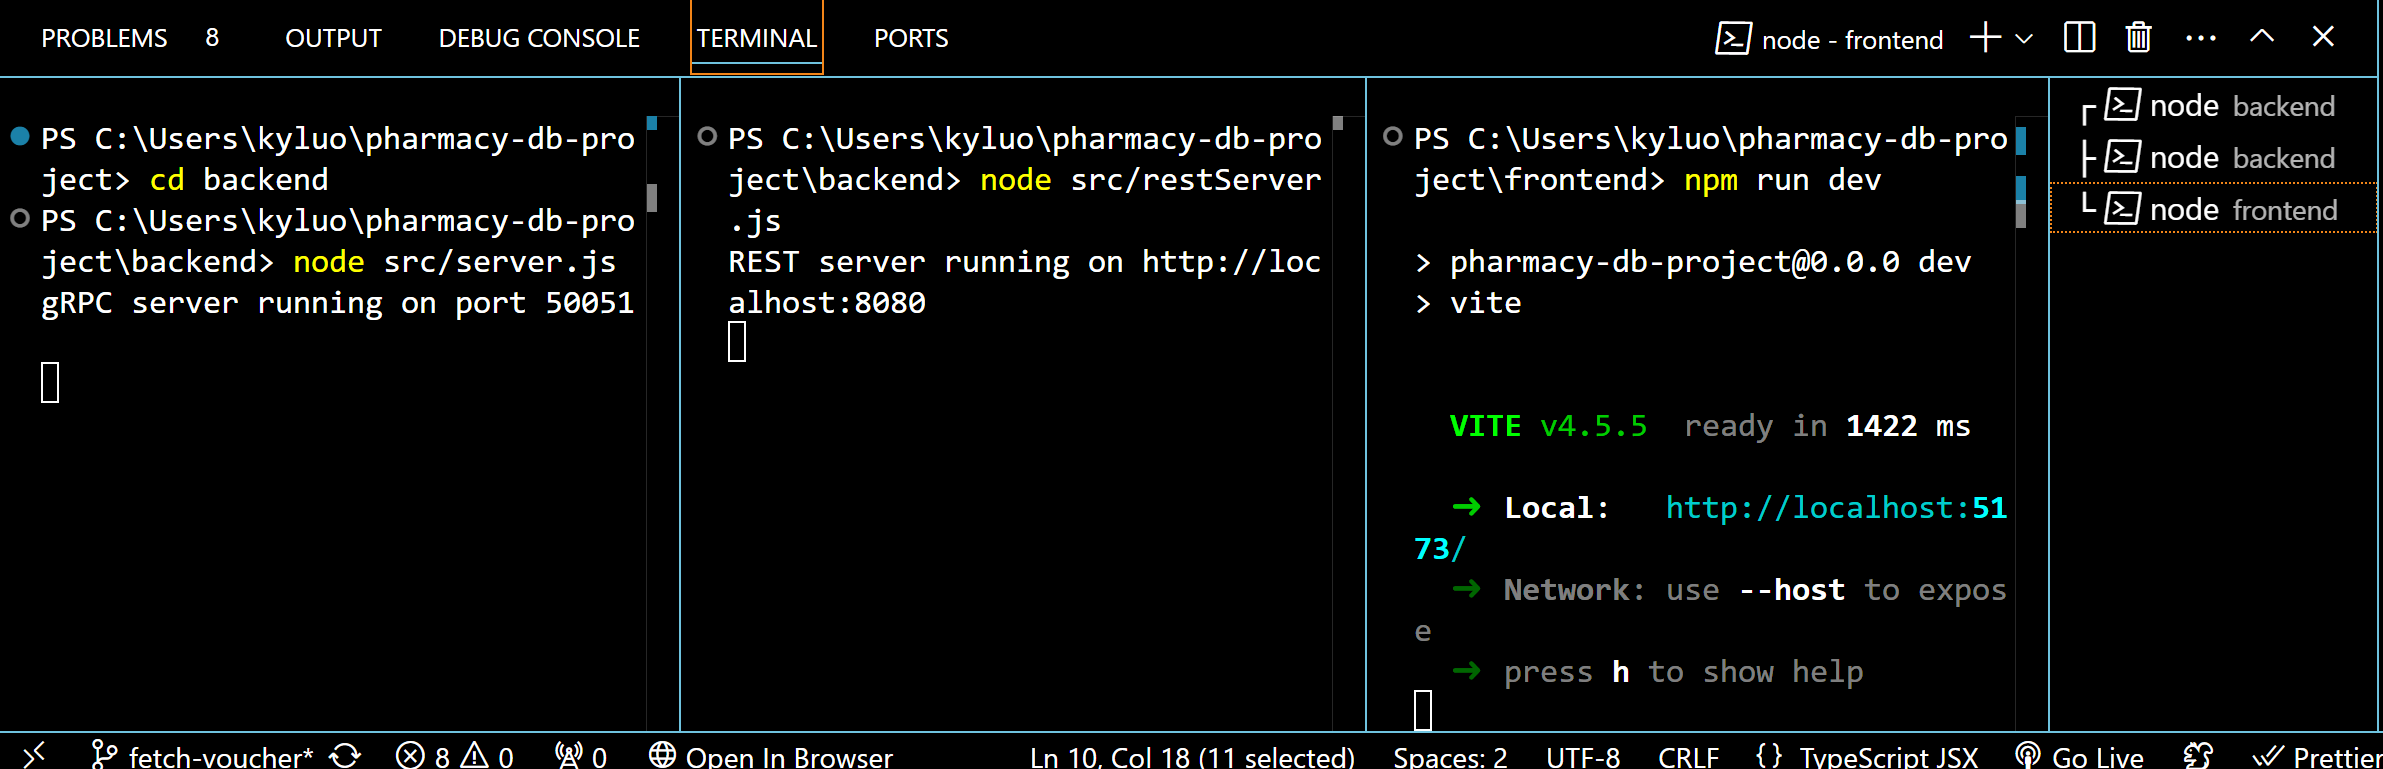
\includegraphics[scale=0.35]{Images/Screenshot 2024-12-23 152956.png}
\end{figure}
\textbf{Trang chủ của hệ thống khi chưa đăng nhập:}
   \begin{figure}[H]
        \hspace*{1cm}     
            
\includegraphics[scale=0.3]{Images/dnhap.png}
        \end{figure}

      \begin{figure}[H]
        \hspace*{1cm}     
            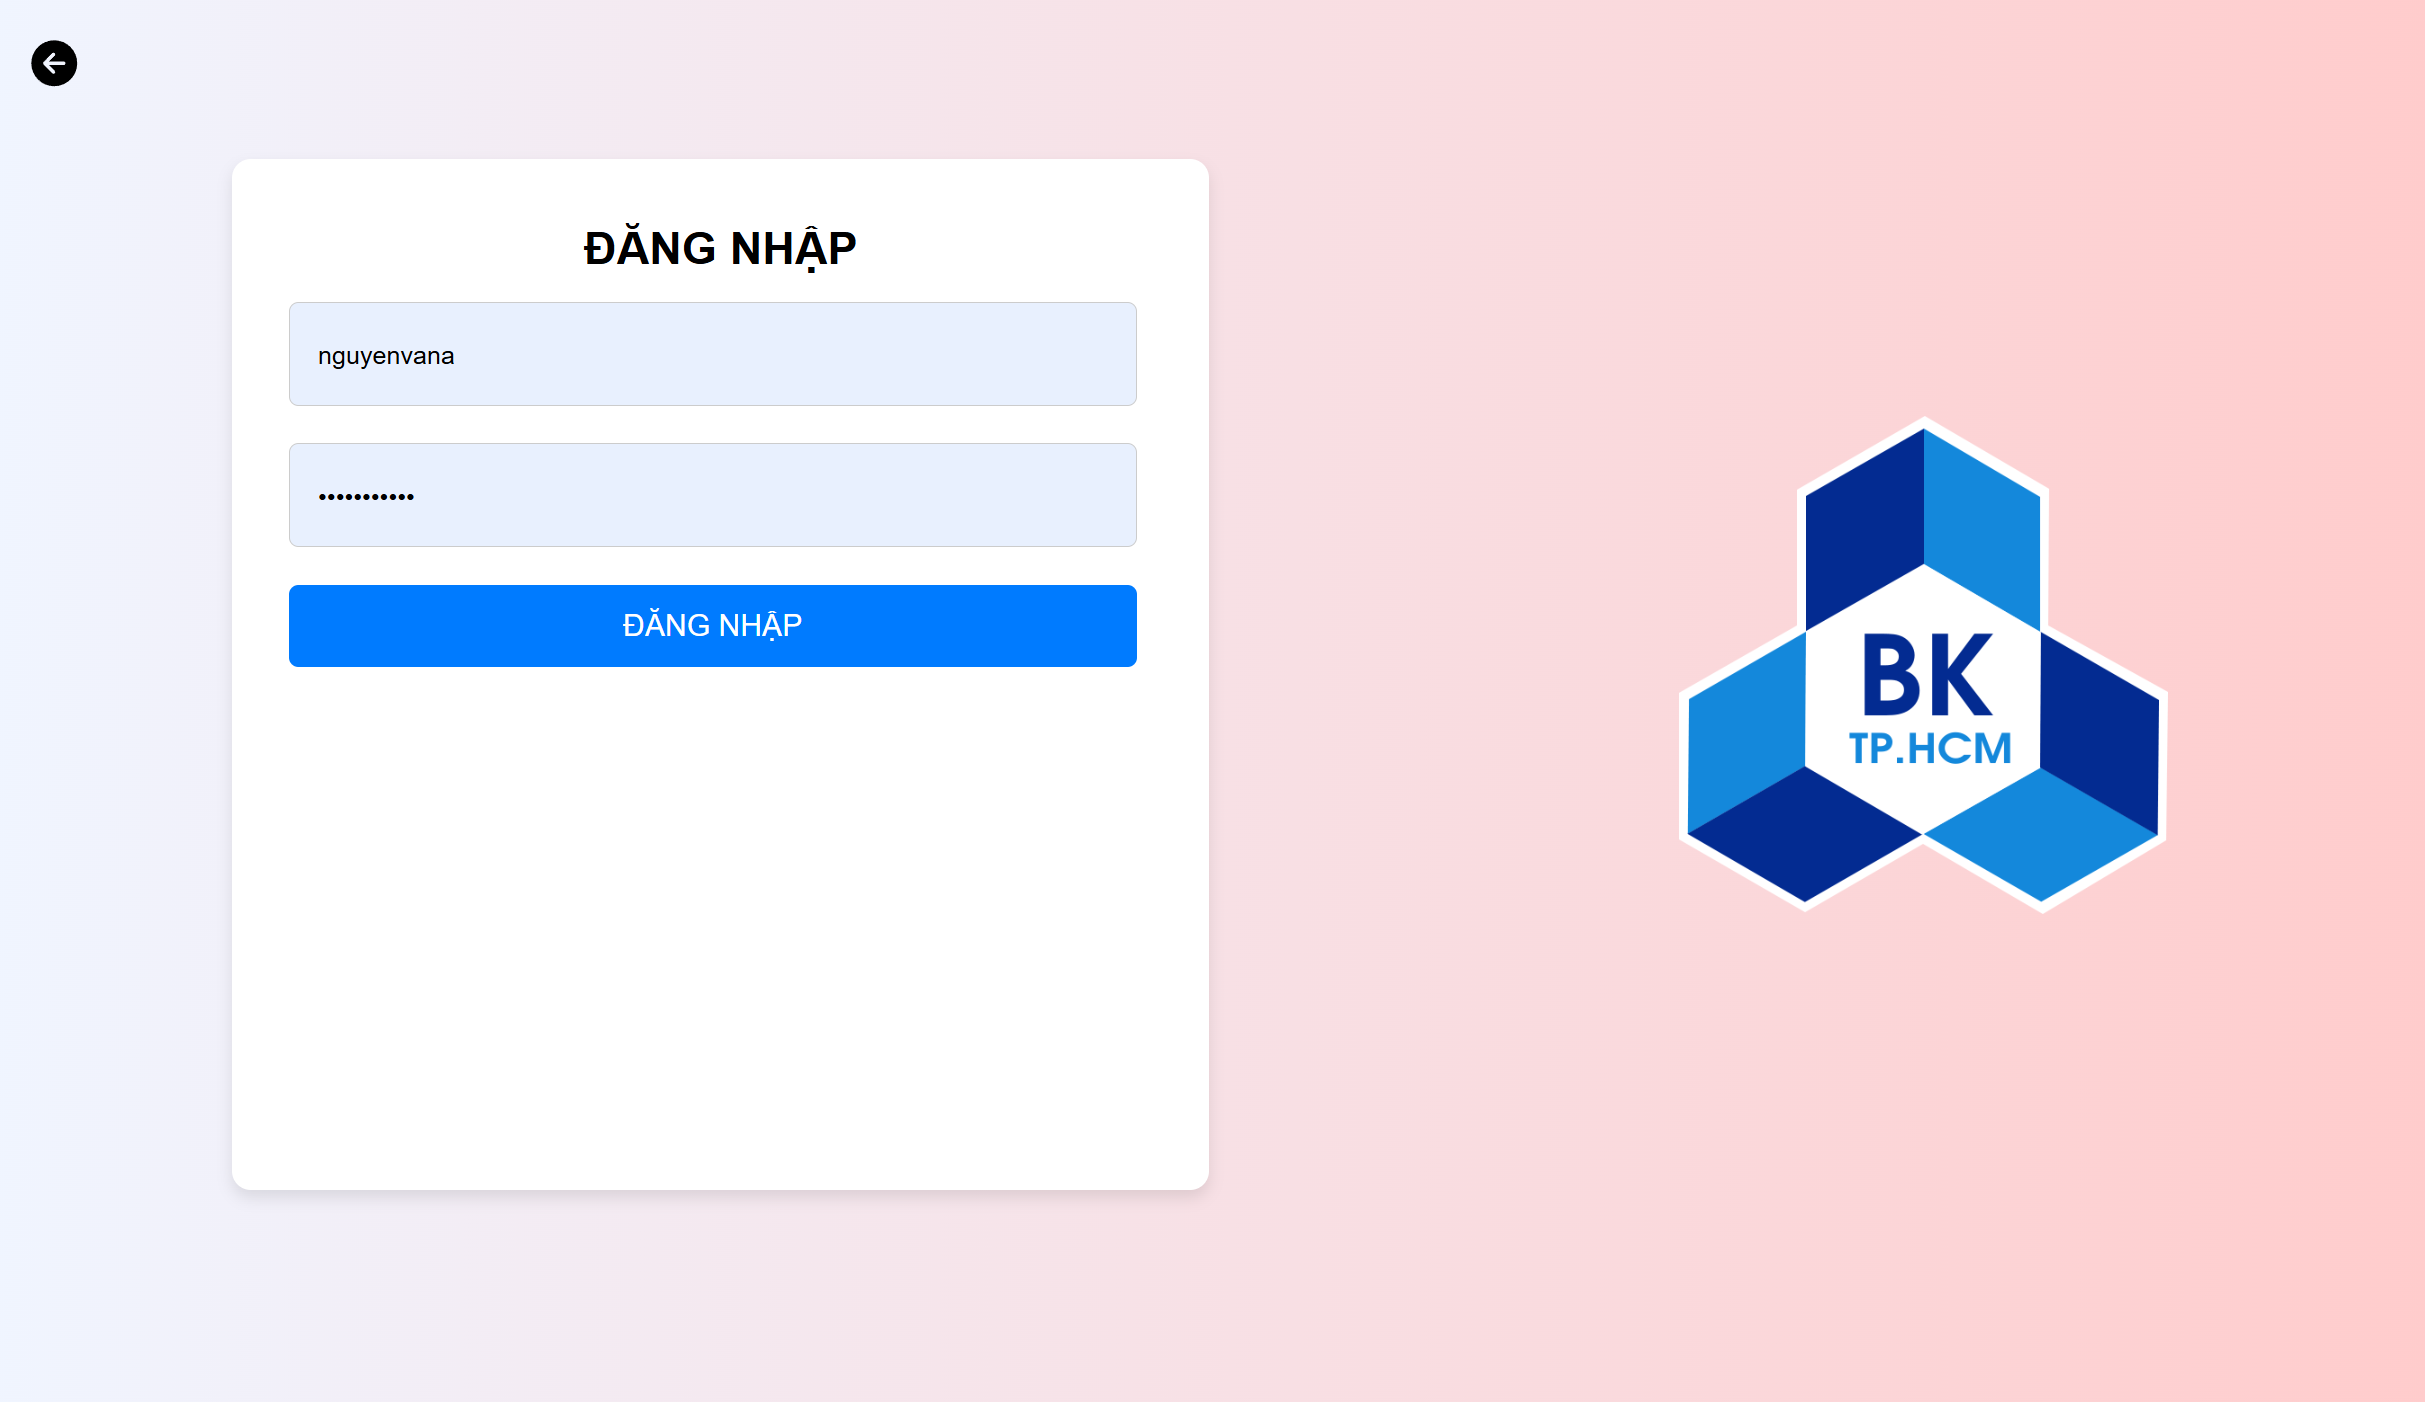
\includegraphics[scale=0.3]{Images/signin.png}
        \end{figure}
Hệ thống dành cho 4 người dùng chủ yếu ứng với các thanh menu riêng biệt:
\begin{itemize}
      \item \textbf{Admin (Người quản lý): }
        \begin{figure}[H]
        \hspace*{1cm}     
            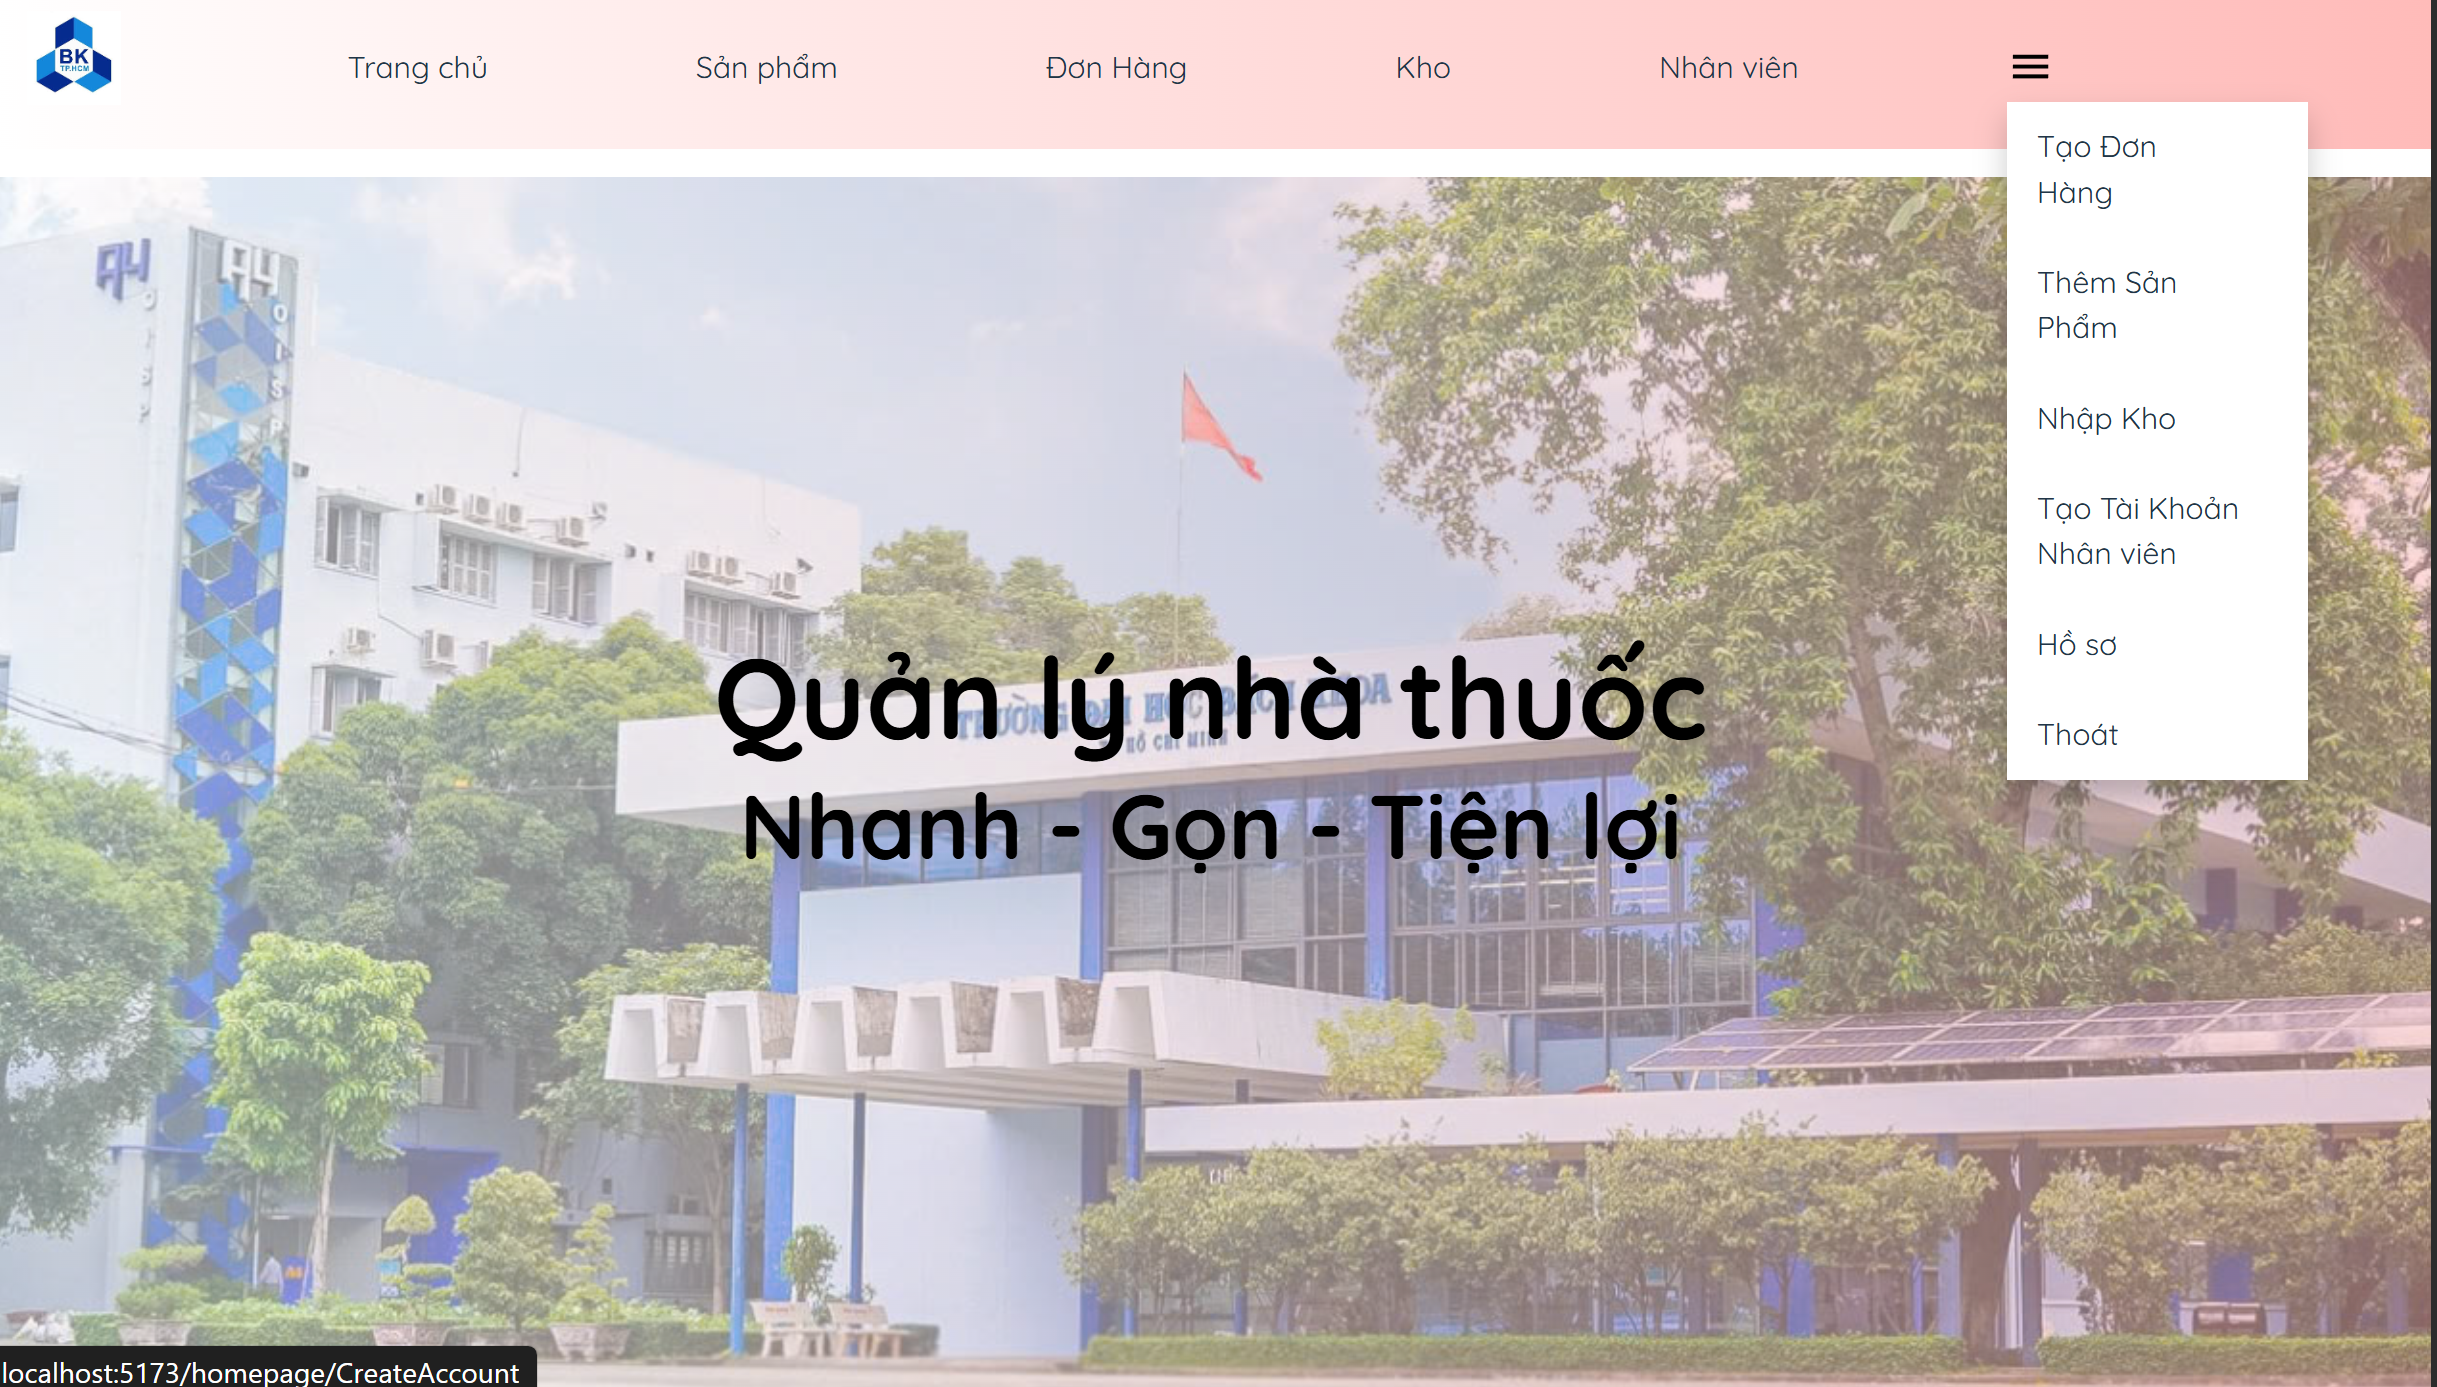
\includegraphics[scale=0.3]{Images/hp2.png}
        \end{figure}
        
      \item \textbf{Người quản lý sản phẩm: }
        \begin{figure}[H]
        \hspace*{1cm}     
            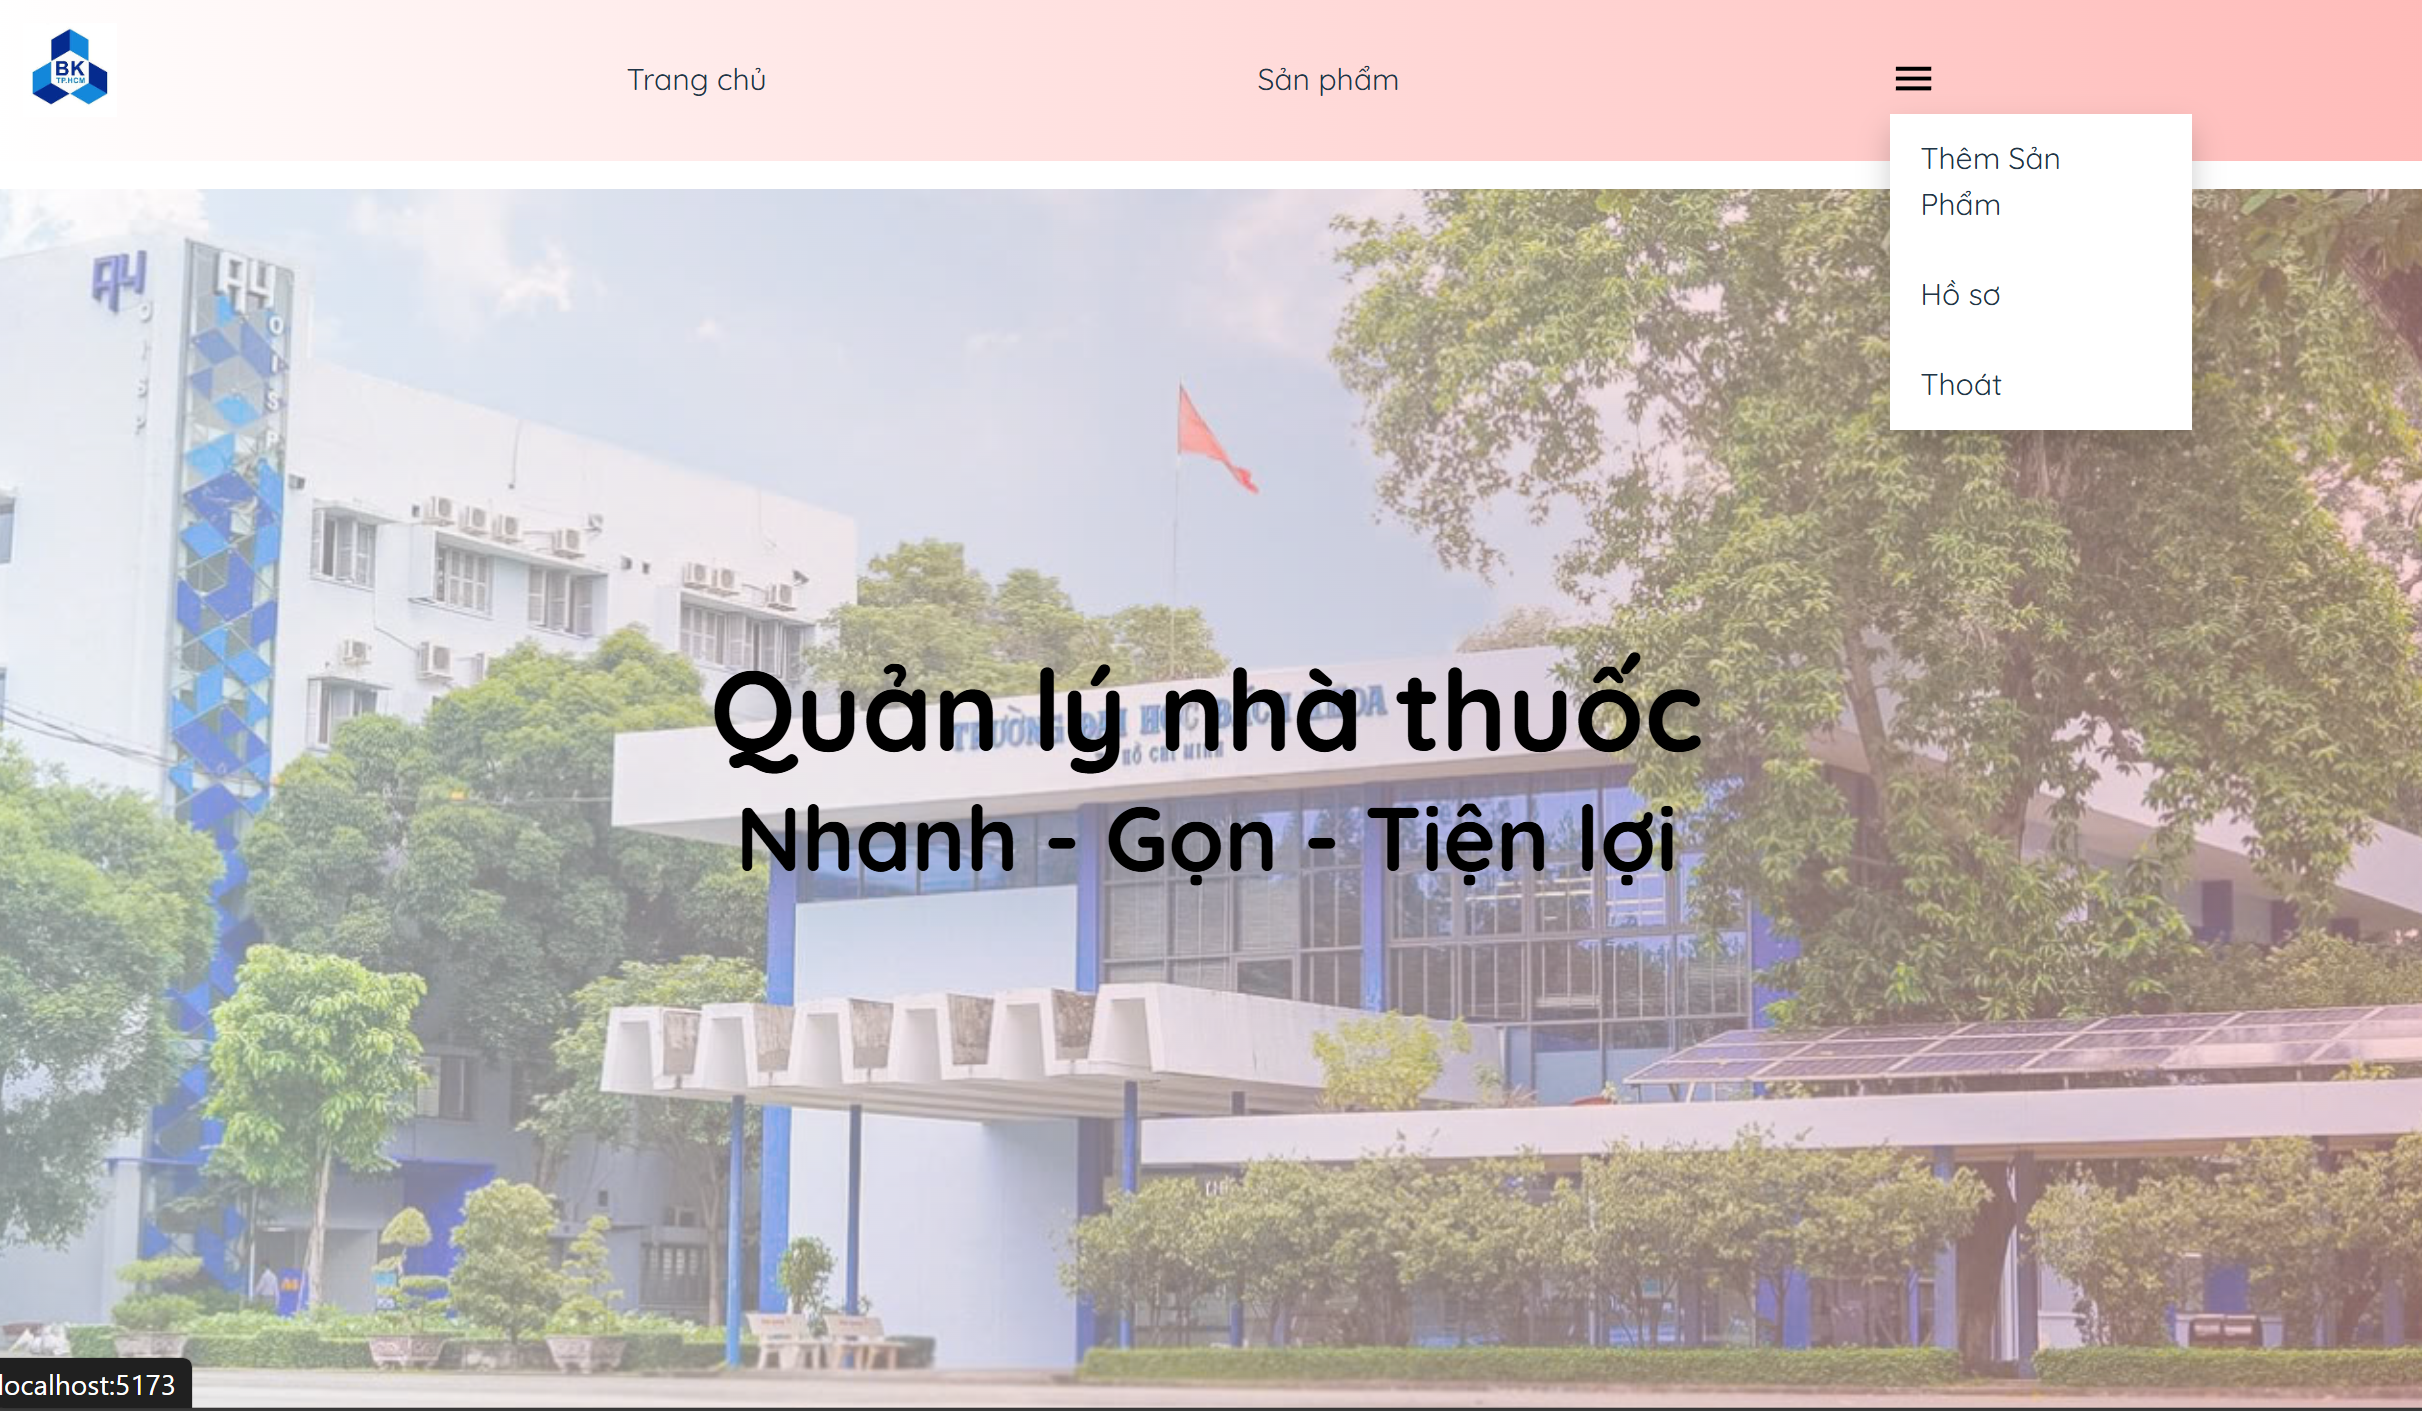
\includegraphics[scale=0.3]{Images/hp_prod.png}
        \end{figure}
        
      \item \textbf{Người quản kho: }
        \begin{figure}[H]
        \hspace*{1cm}     
            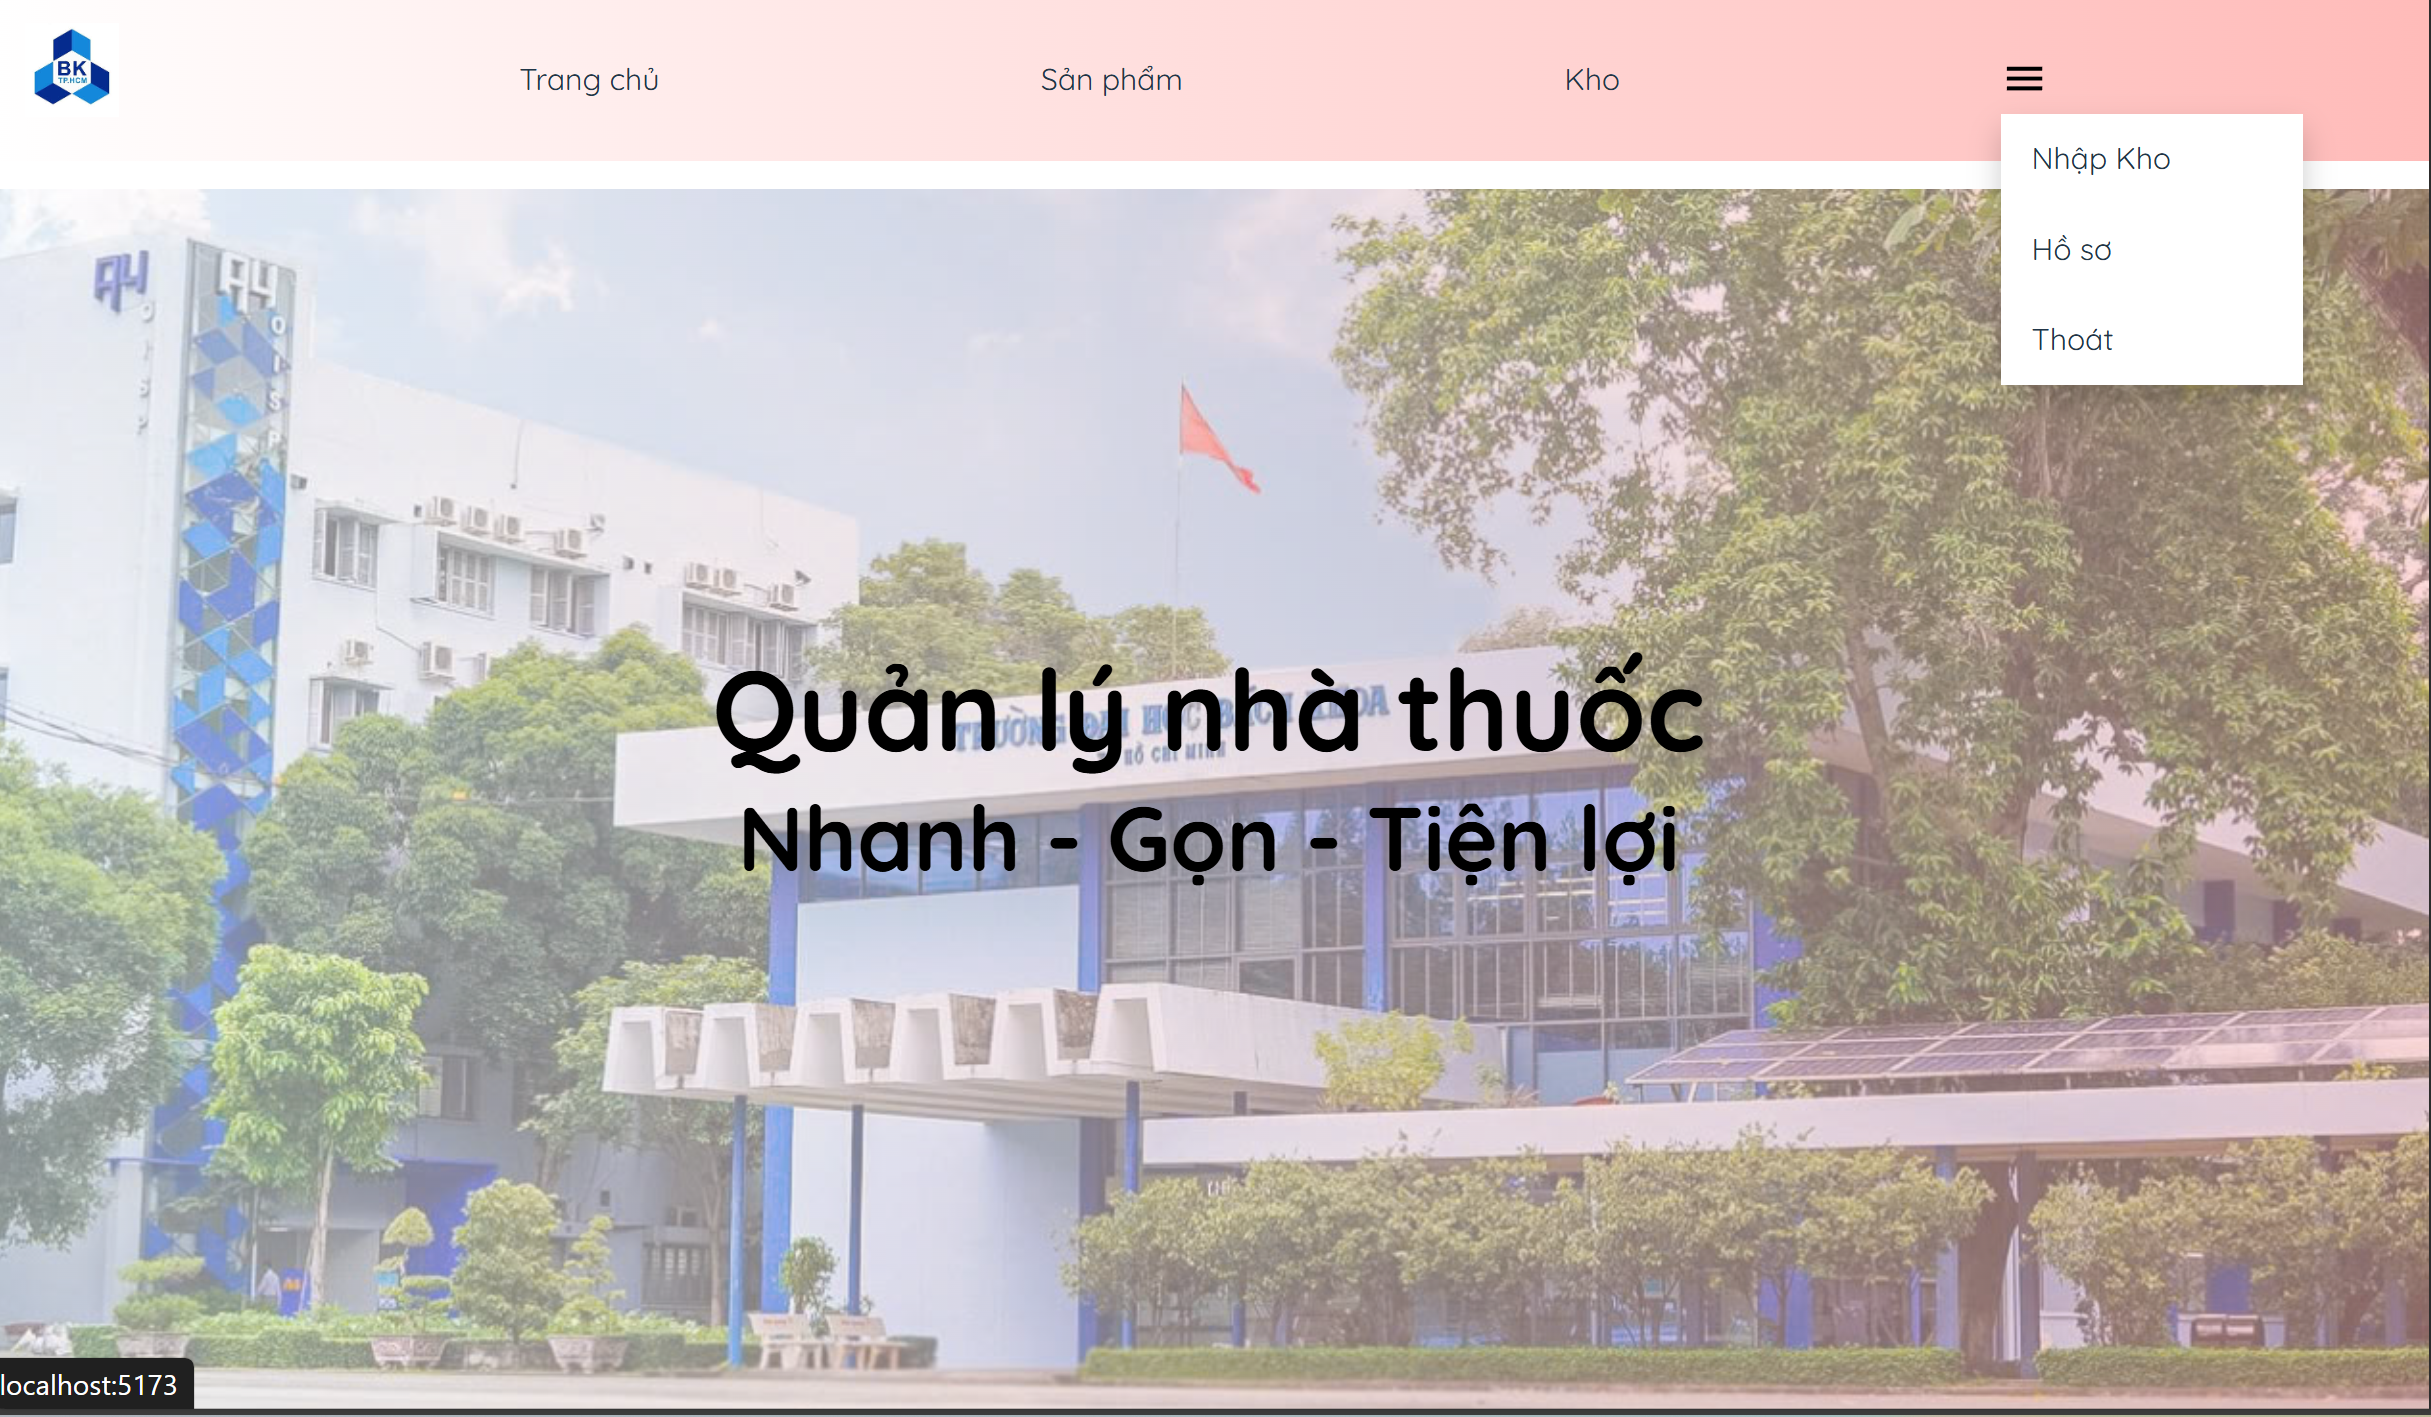
\includegraphics[scale=0.3]{Images/hp_inven.png}
        \end{figure}

     \item \textbf{Nhân viên bán thuốc: }
        \begin{figure}[H]
        \hspace*{1cm}     
            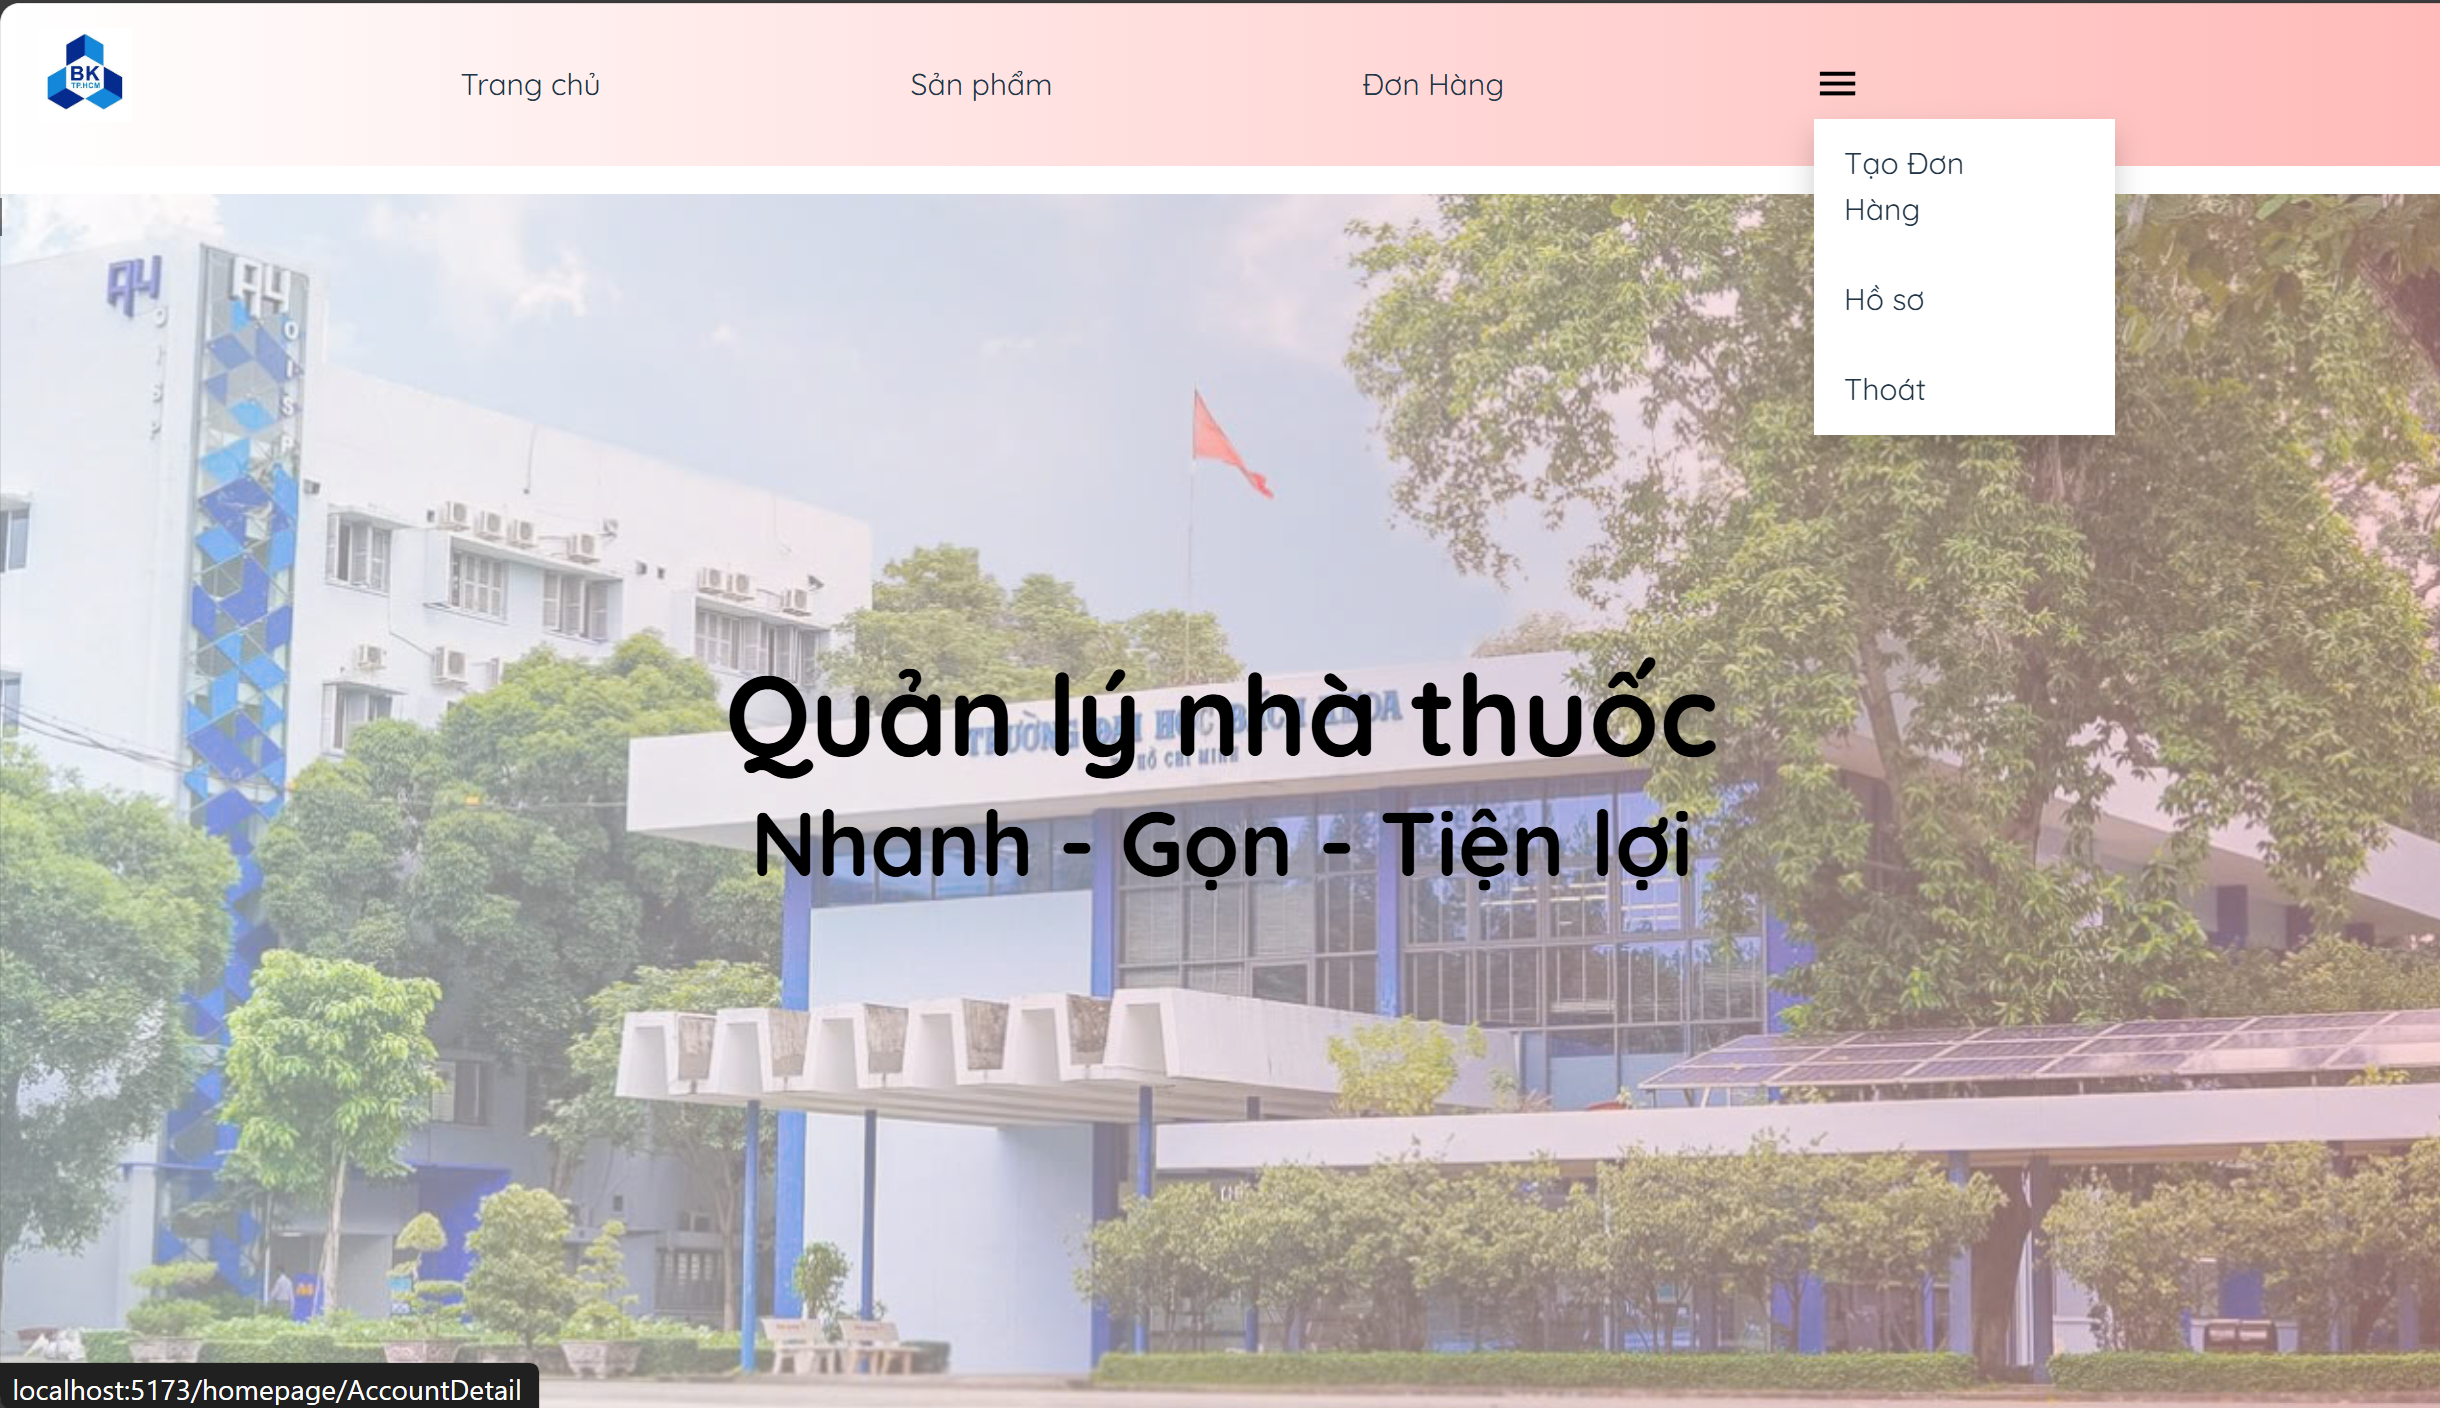
\includegraphics[scale=0.3]{Images/hp_pharmacist.png}
        \end{figure}
\end{itemize}
\subsection{Nhân viên}
Tại trang nhân viên sẽ hiển thị các tài khoản của nhân viên trong hệ thống kèm các chức năng:
\begin{itemize}
    \item Tìm kiếm nhân viên:
     \begin{figure}[H]
        \hspace*{1cm}     
            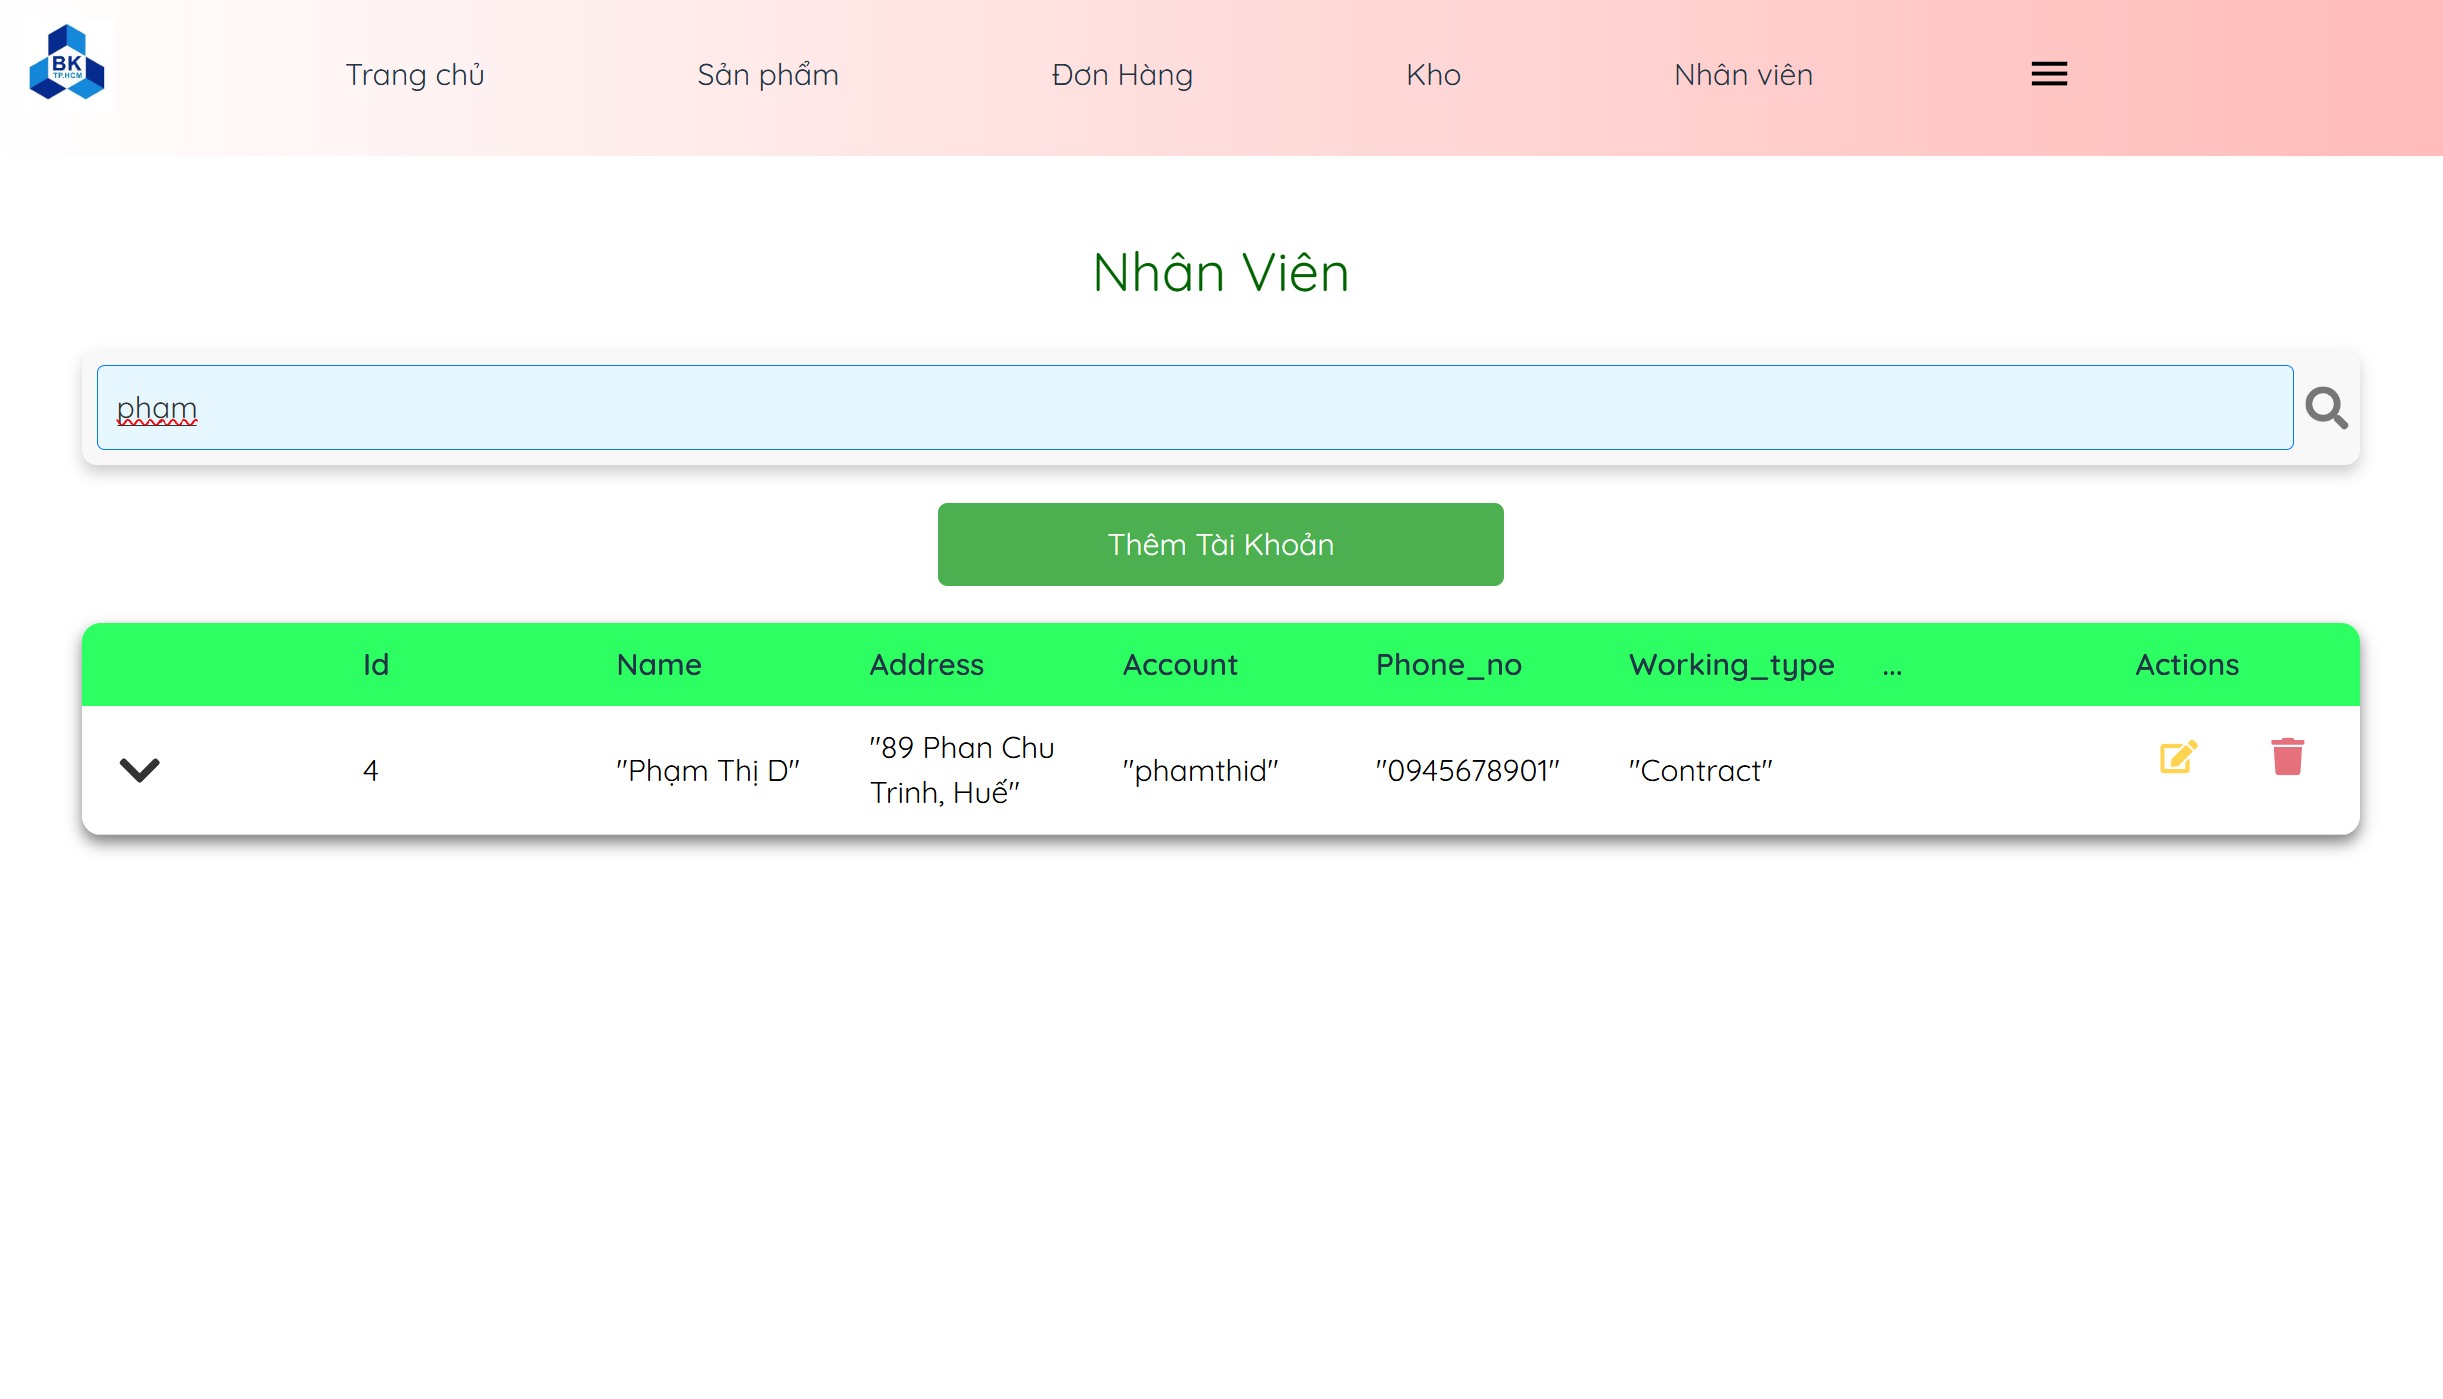
\includegraphics[scale=0.3]{Images/search_nv.png}
        \end{figure}
    \item Xóa nhân viên:
     \begin{figure}[H]
        \hspace*{1cm}     
            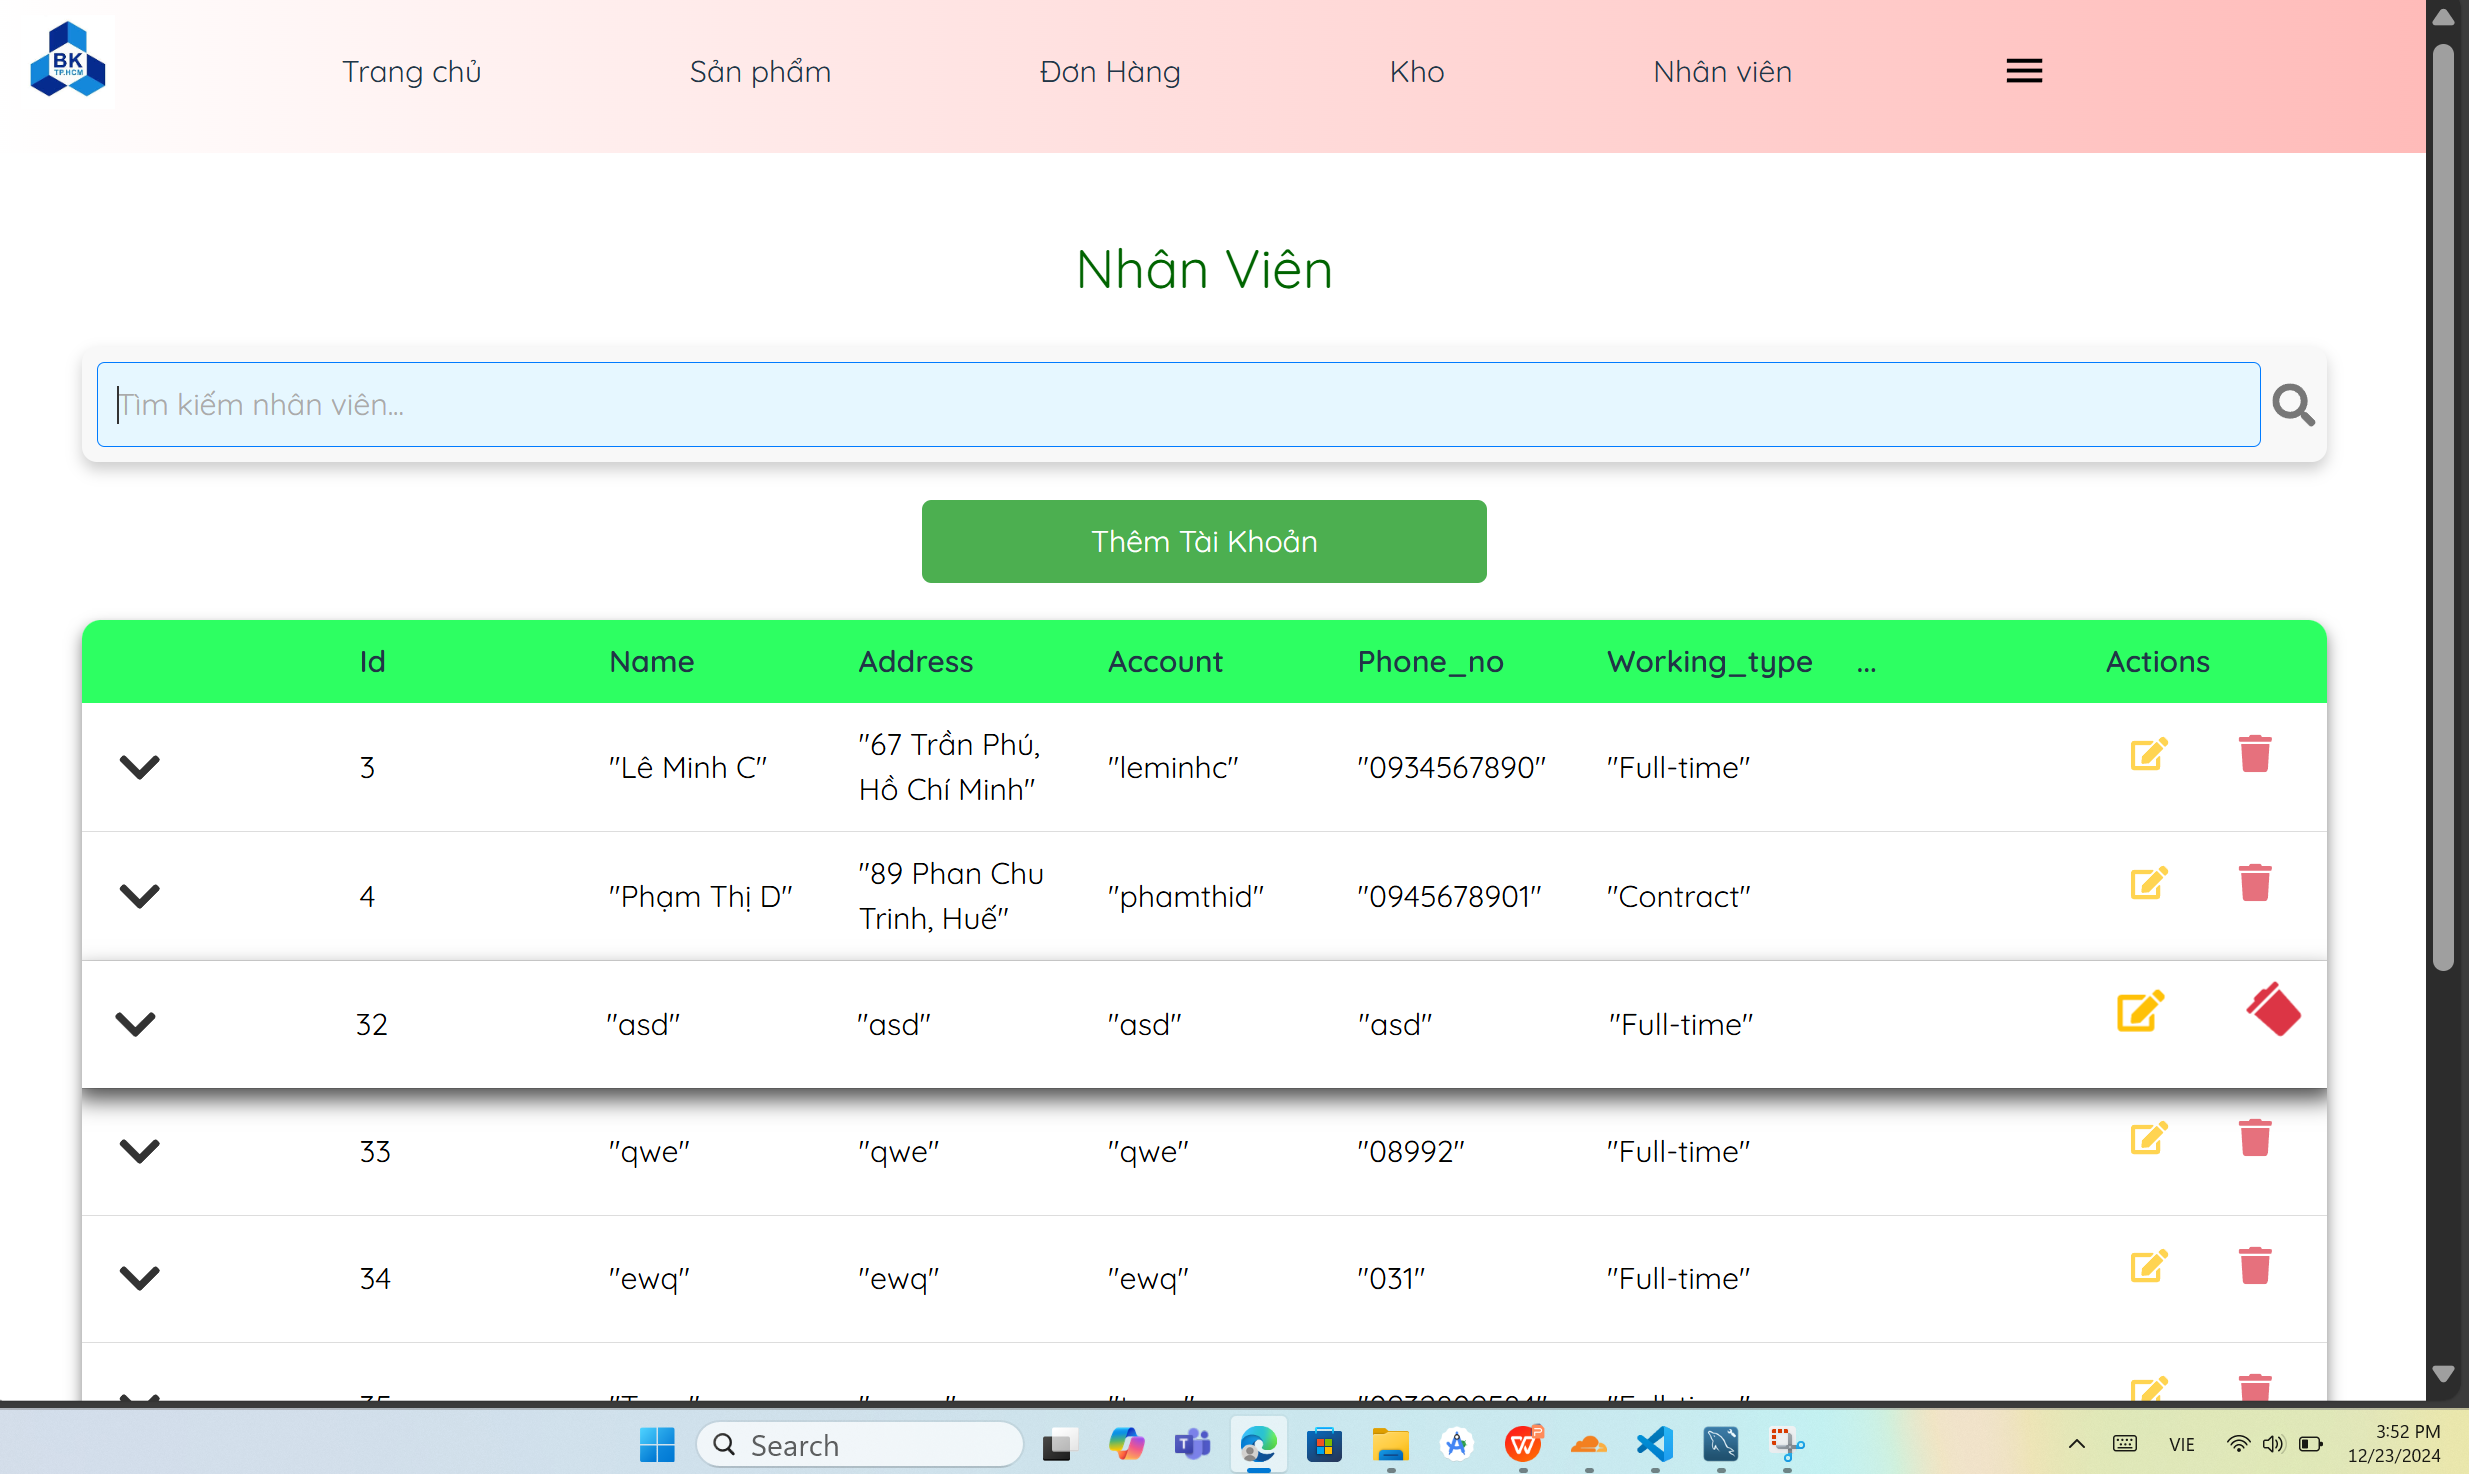
\includegraphics[scale=0.3]{Images/xoanv.png}
        \end{figure}
        Nhân viên đã được xóa thành công:
        \begin{figure}[H]
        \hspace*{1cm}     
            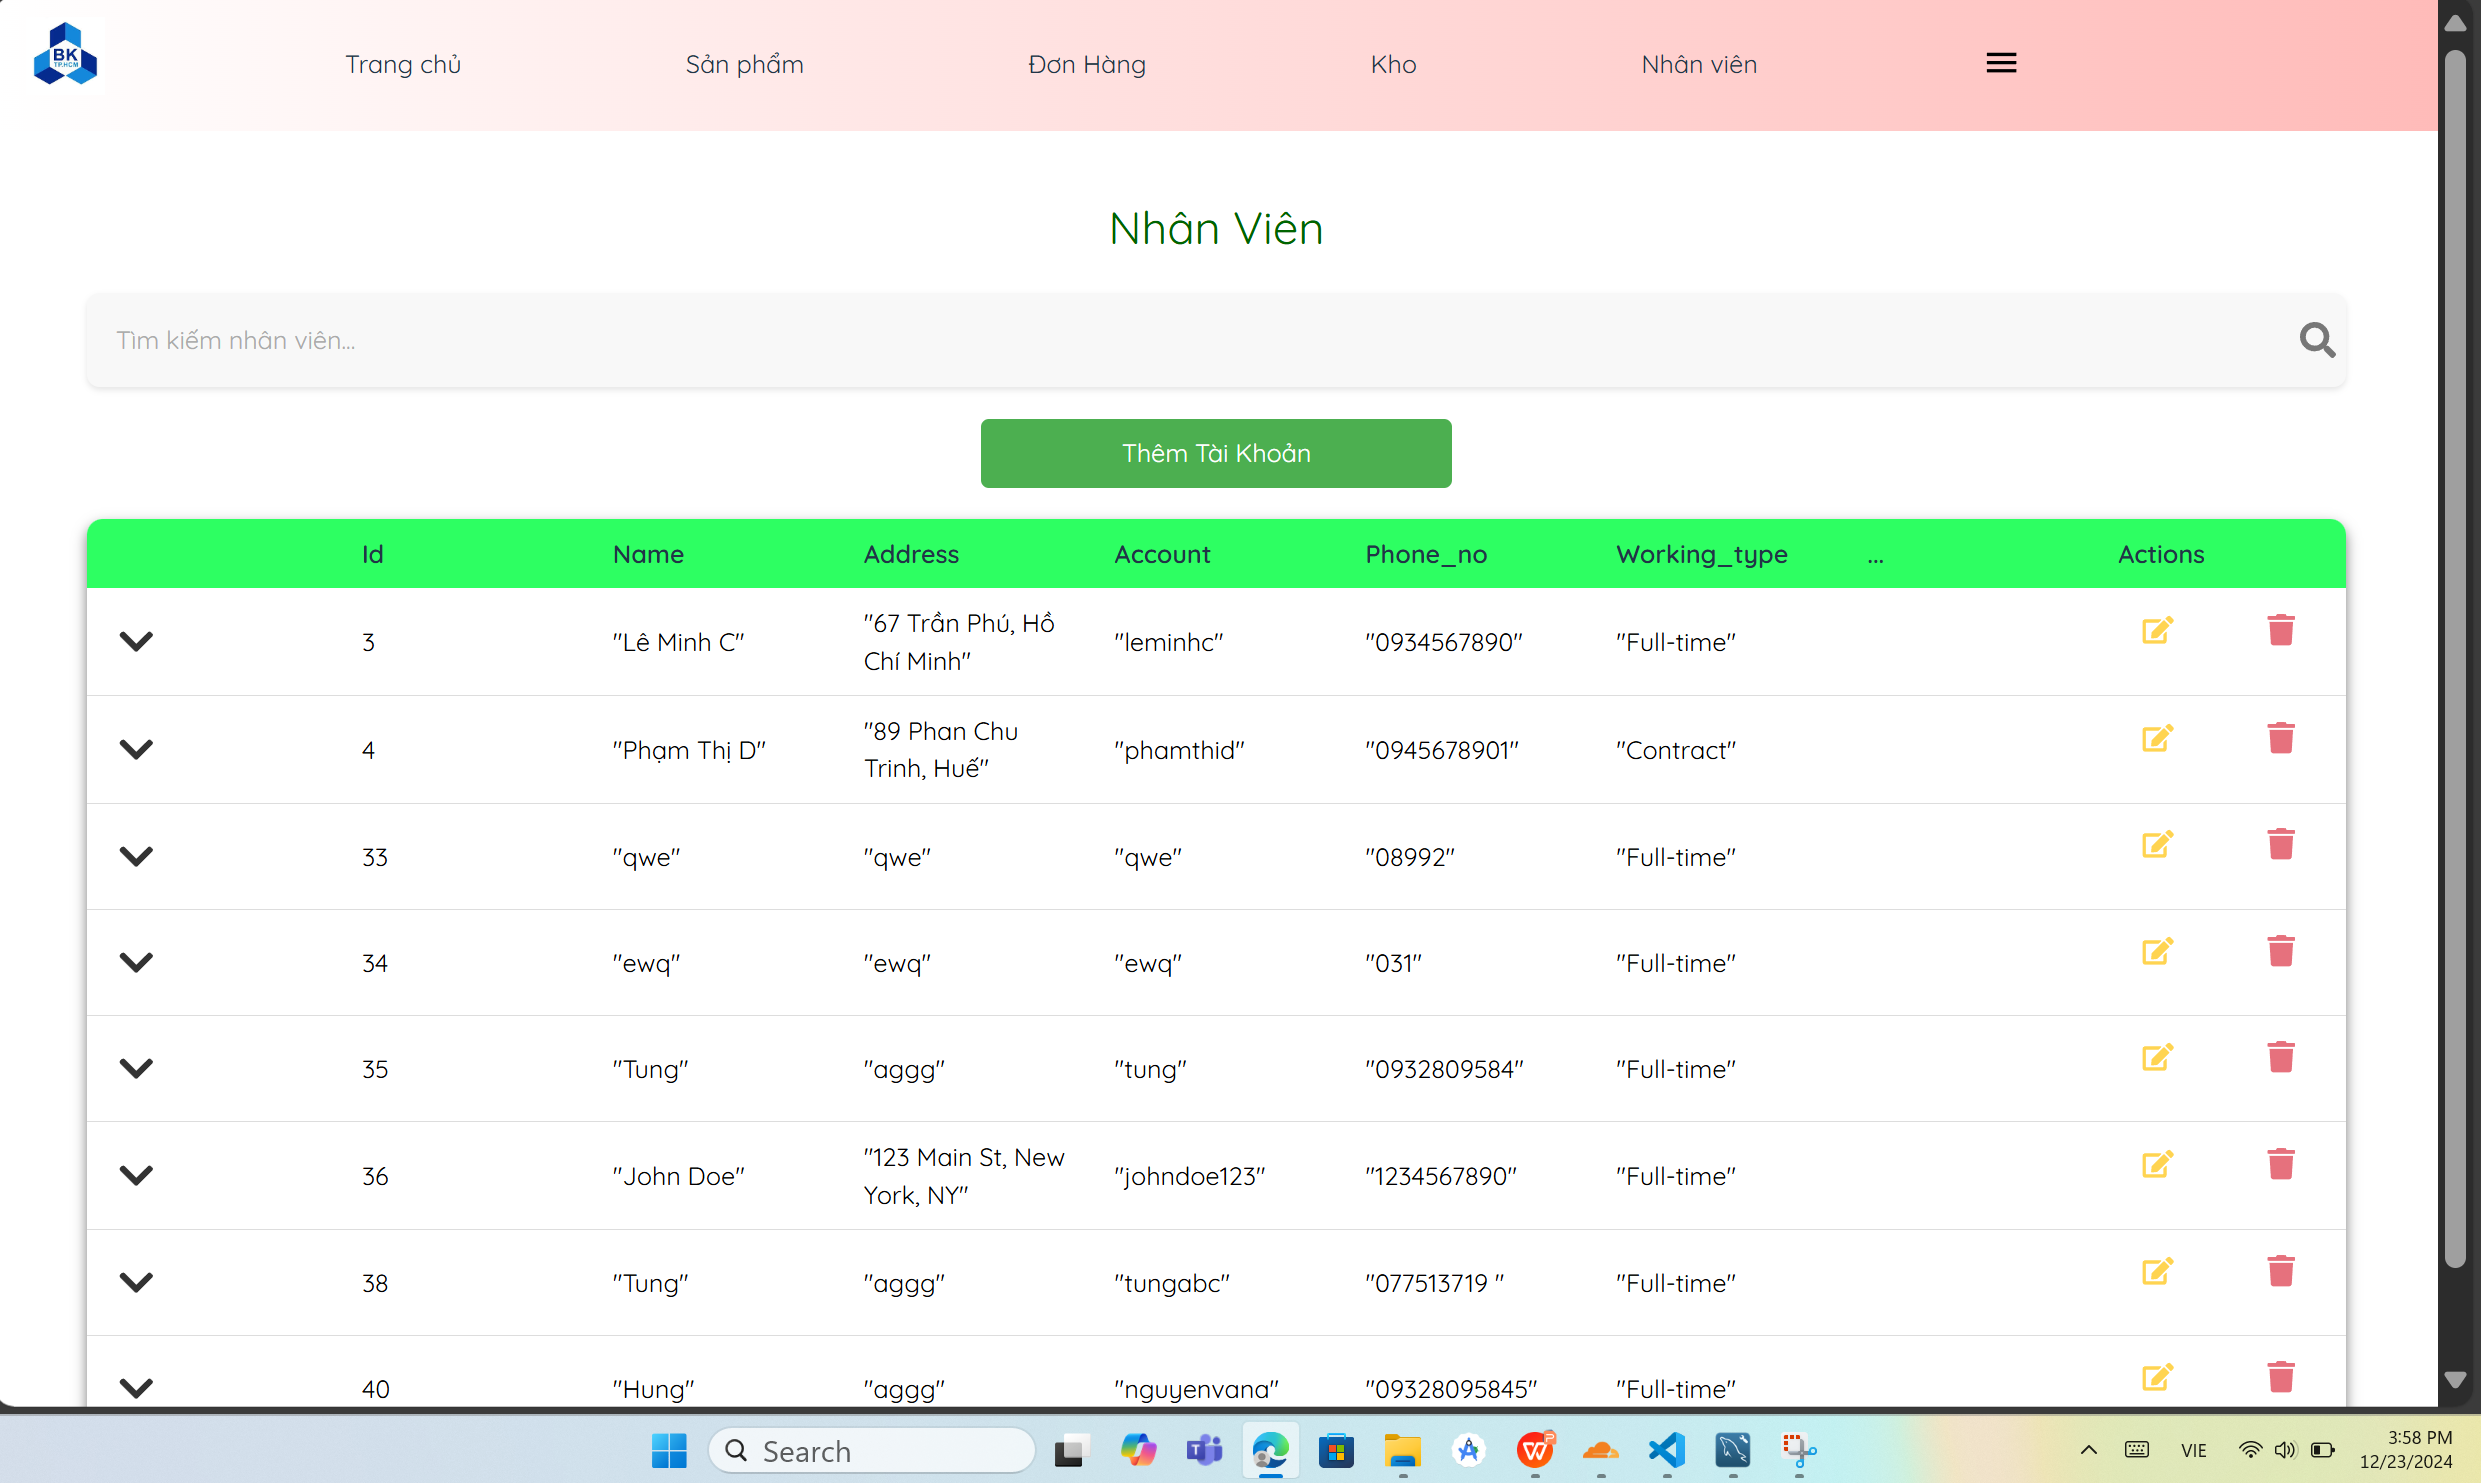
\includegraphics[scale=0.3]{Images/nvbay.png}
        \end{figure}
    \item Sửa thông tin nhân viên:
    \begin{figure}[H]
        \hspace*{-1cm}     
            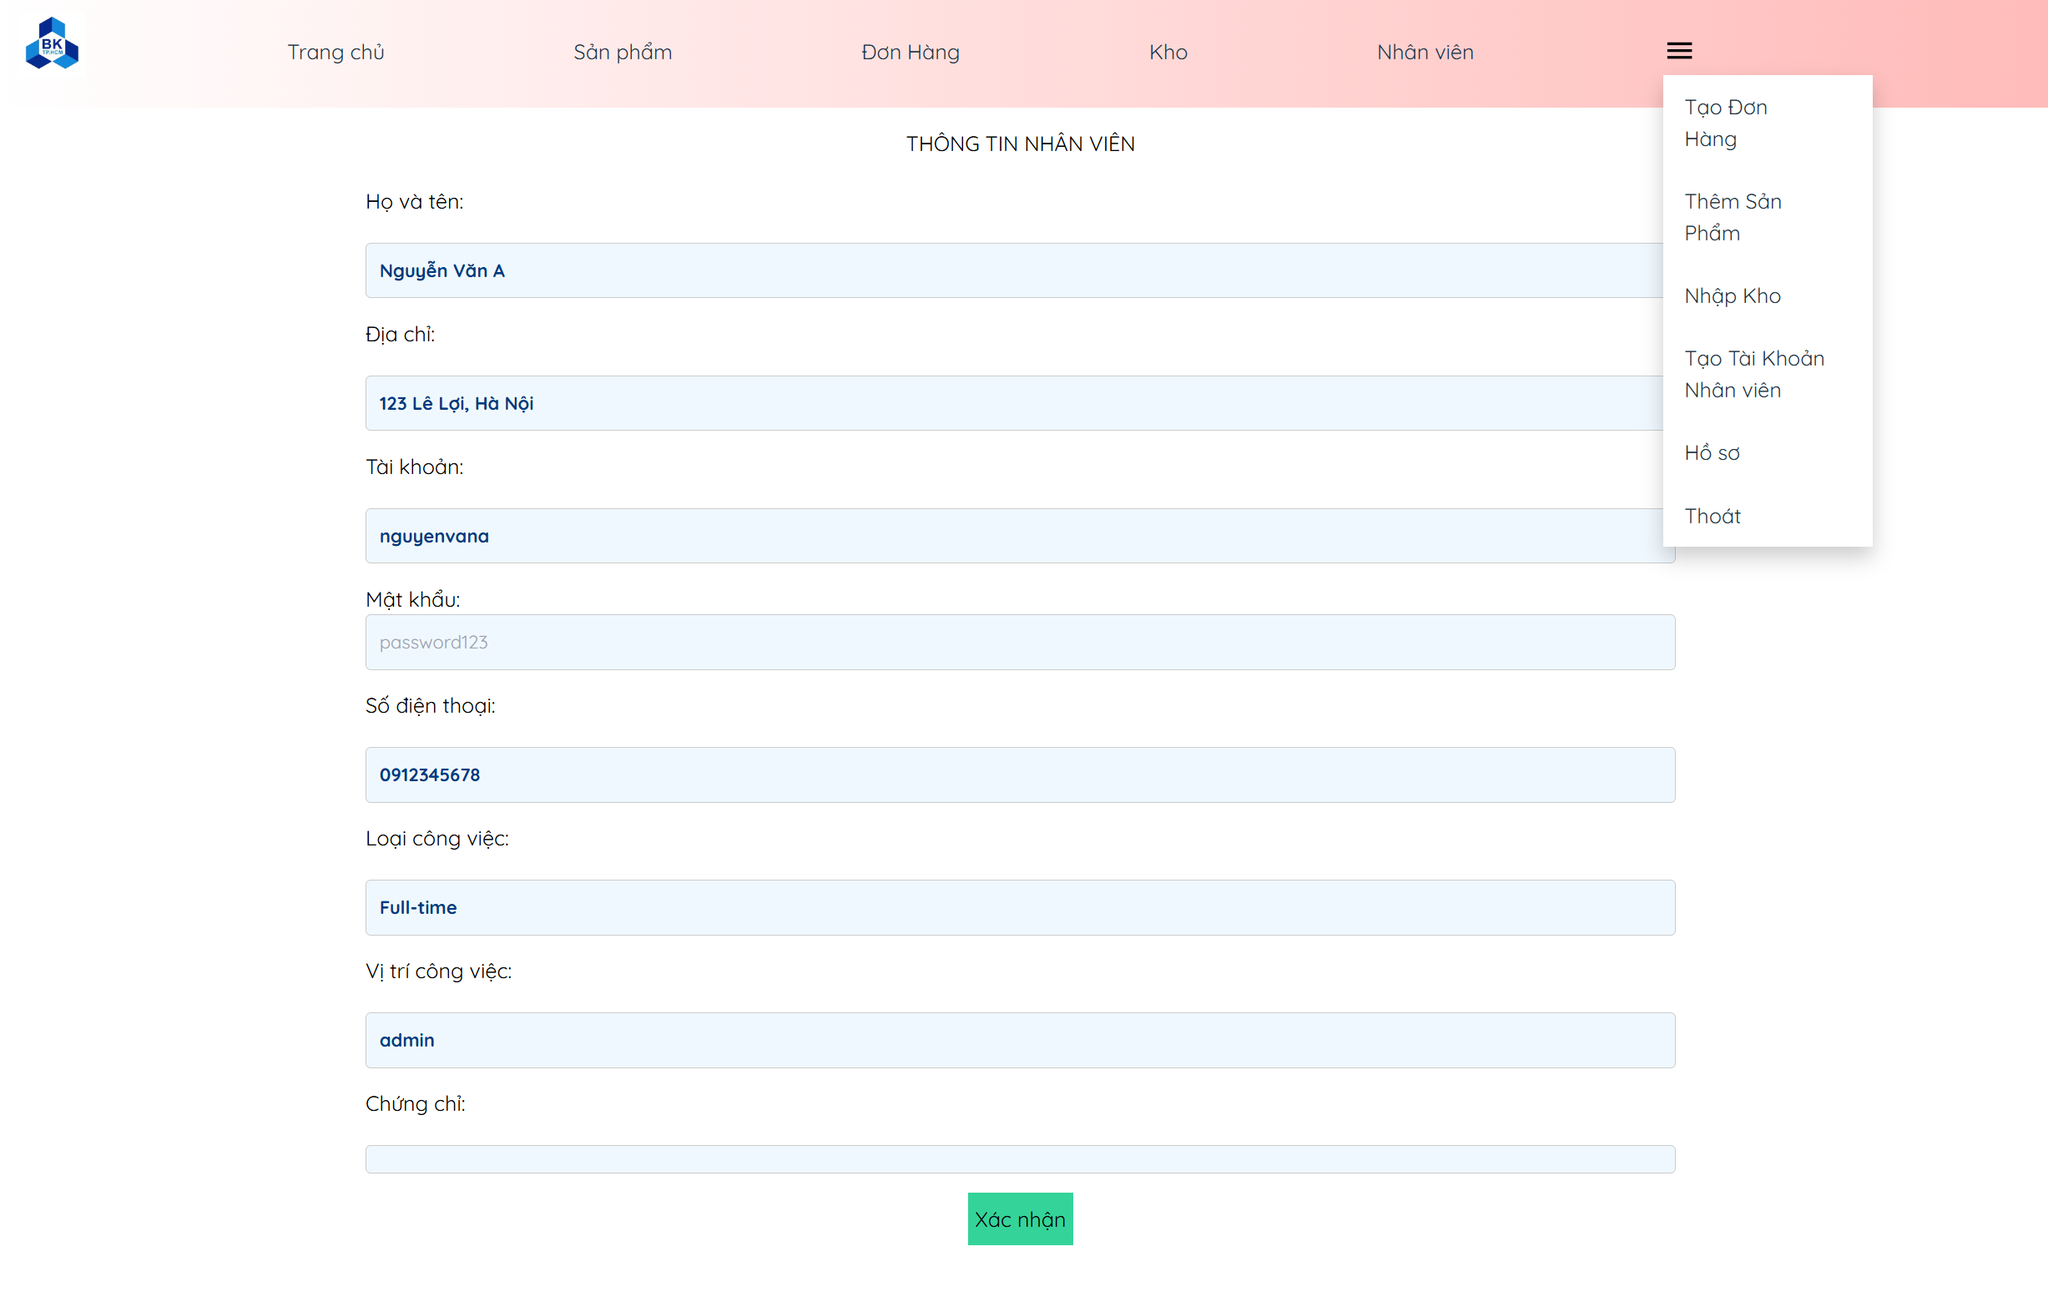
\includegraphics[scale=0.2]{Images/pas_hoso.png}
        \end{figure}
    \item Thêm nhân viên: 

         \begin{figure}[H]
        \hspace*{1cm}     
            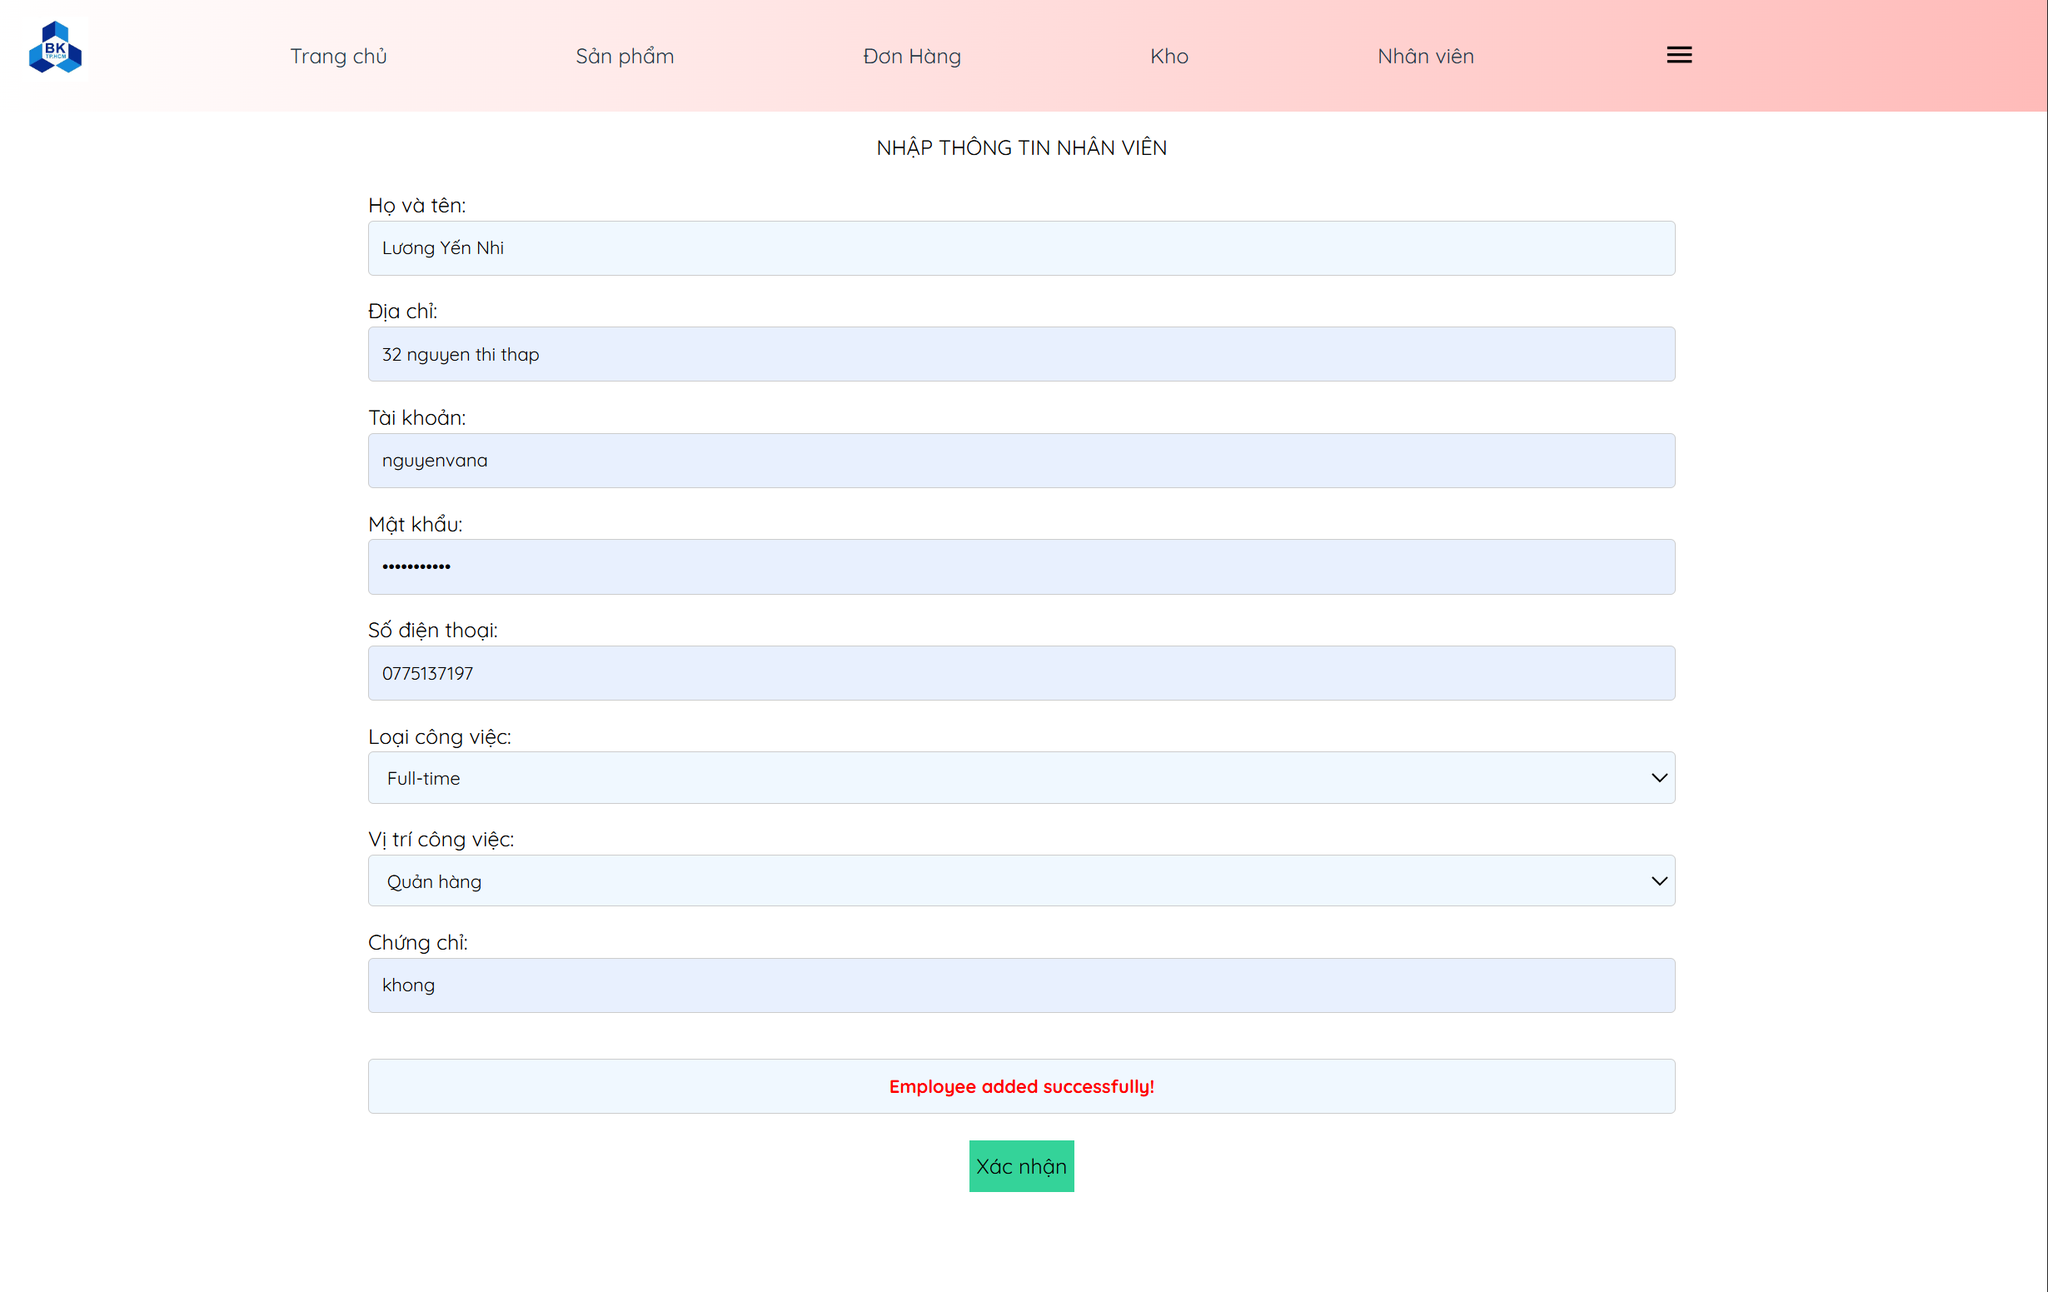
\includegraphics[scale=0.2]{Images/insert_nv_2.png}
        \end{figure}

          \begin{figure}[H]
        \hspace*{1.9cm}     
            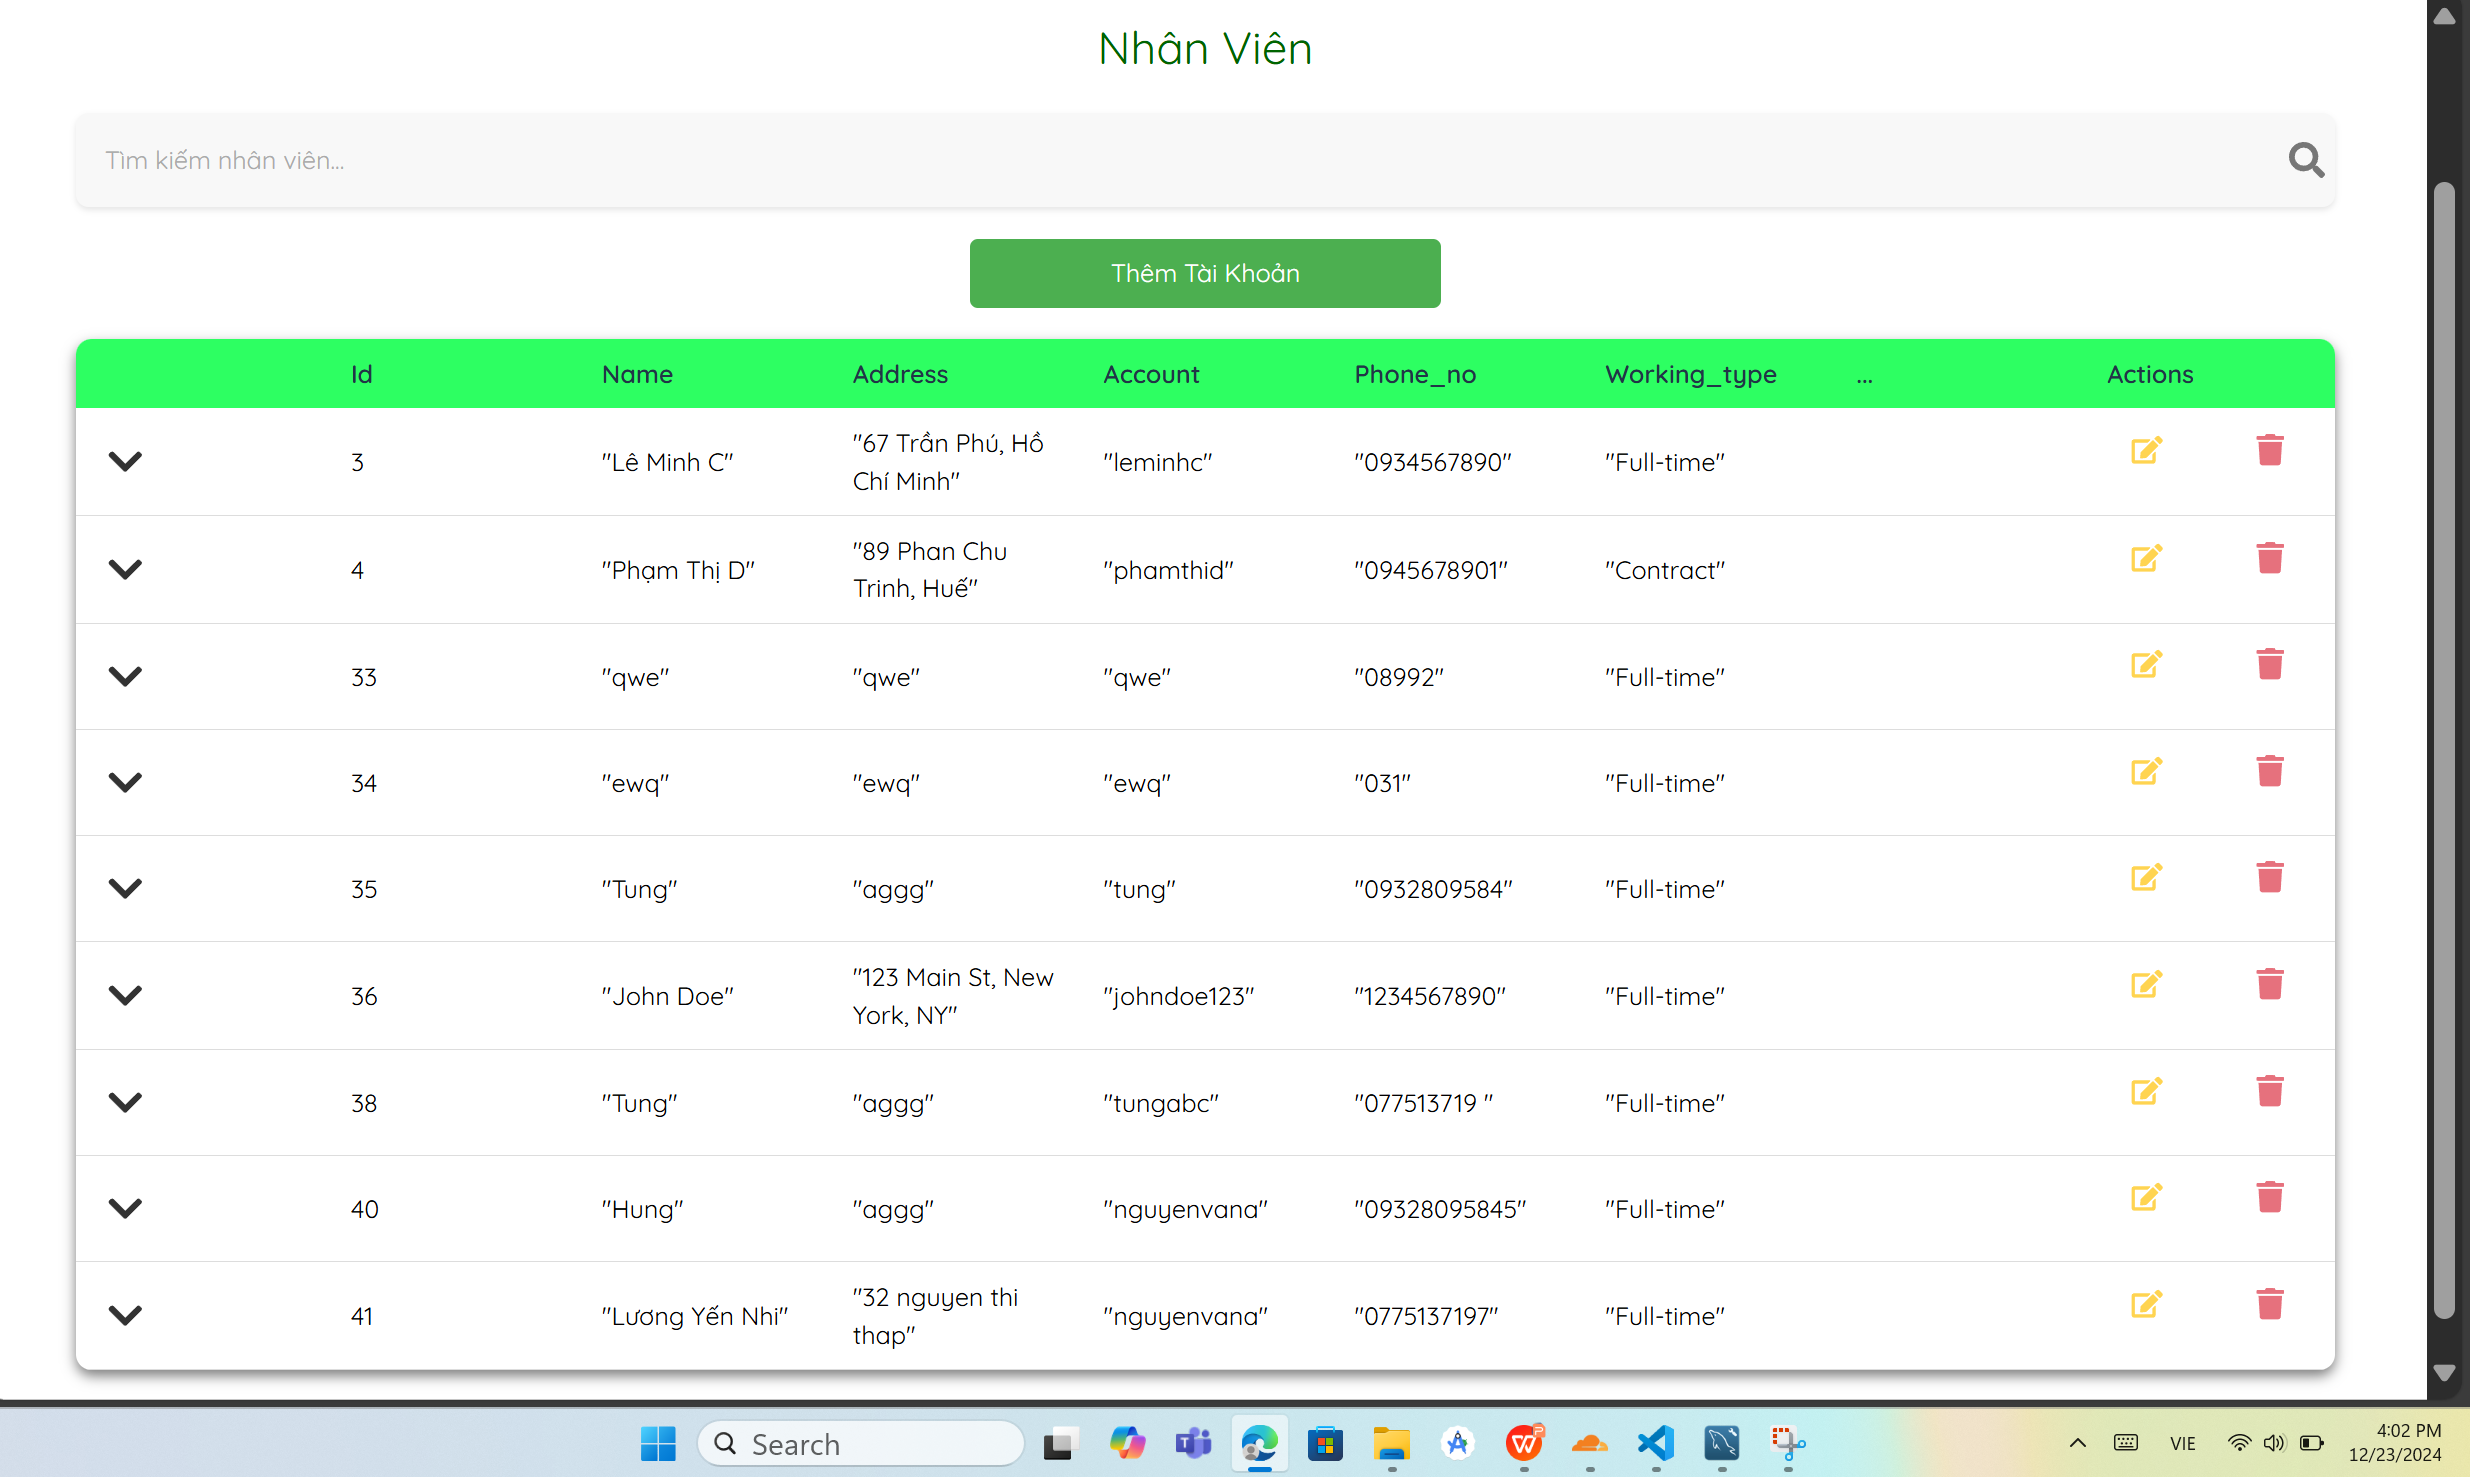
\includegraphics[scale=0.3]{Images/insert_r.png}
        \end{figure}
\end{itemize}
\subsection{Tạo đơn hàng (Nhân viên bán thuốc)}
\textbf{Các đơn hàng đã được tạo trong hệ thống:}
  \begin{figure}[H]  
          \hspace*{1cm}     
            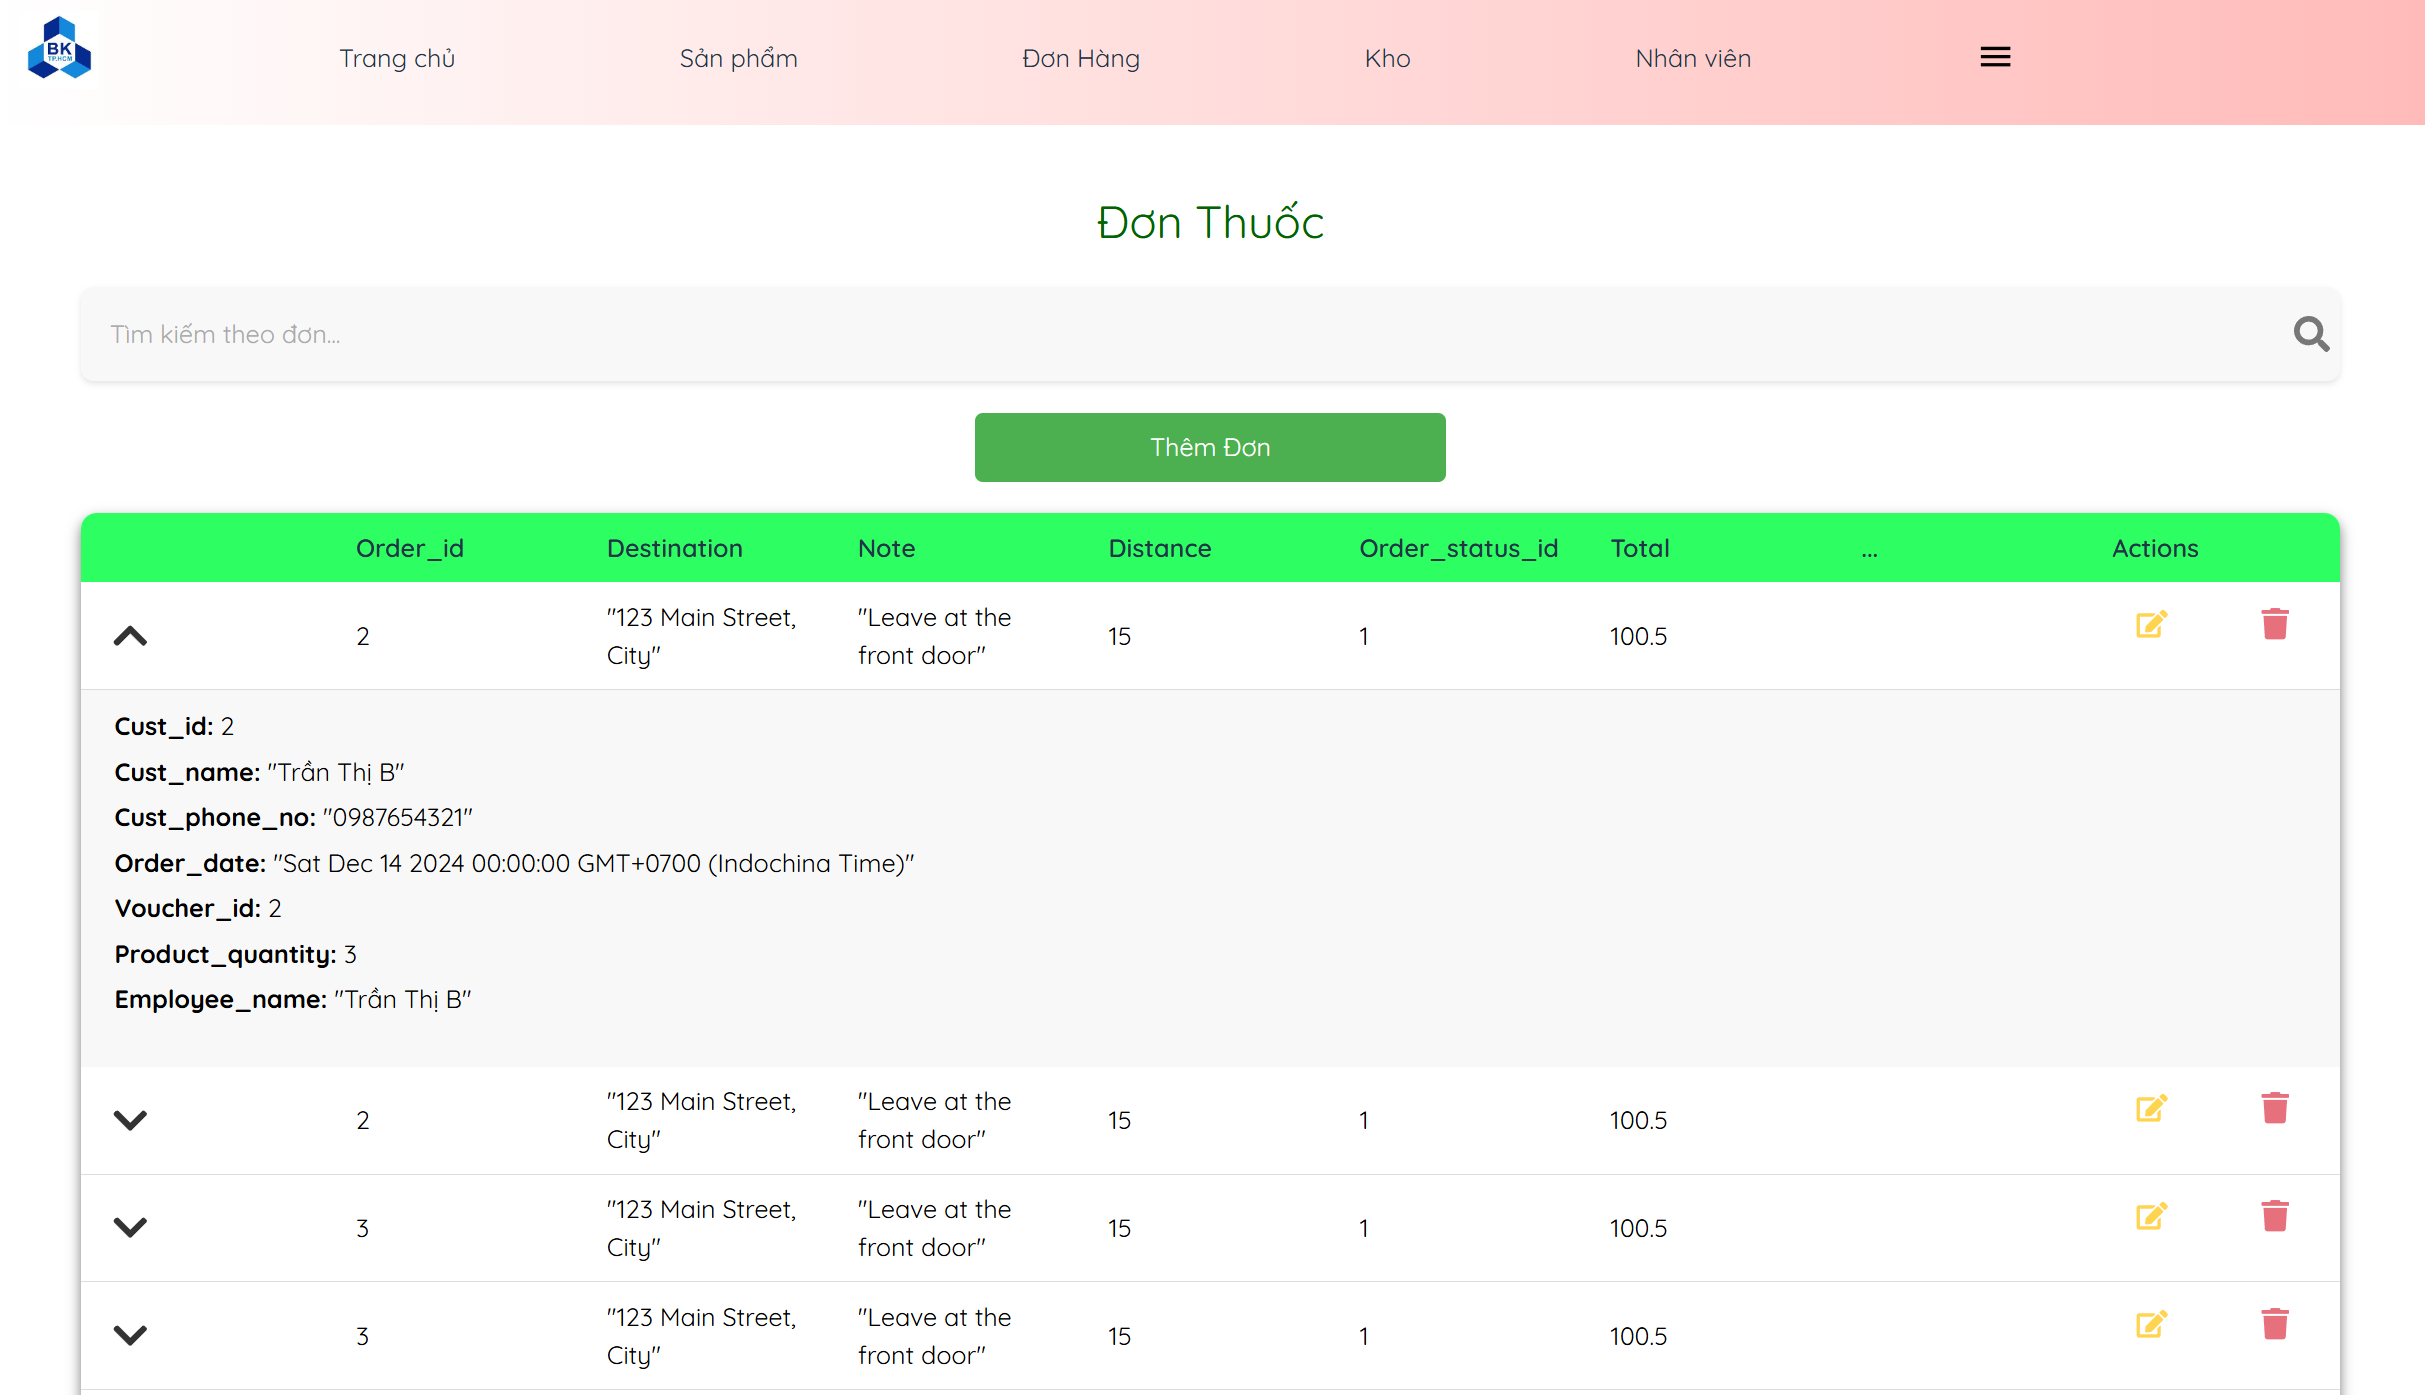
\includegraphics[scale=0.3]{Images/showdon.png}
        \end{figure}
Để thuận tiện, hệ thống sẽ cho người dùng chọn trước các sản phẩm mình muốn chọn:
  \begin{figure}[H]
        \hspace*{-1cm}     
            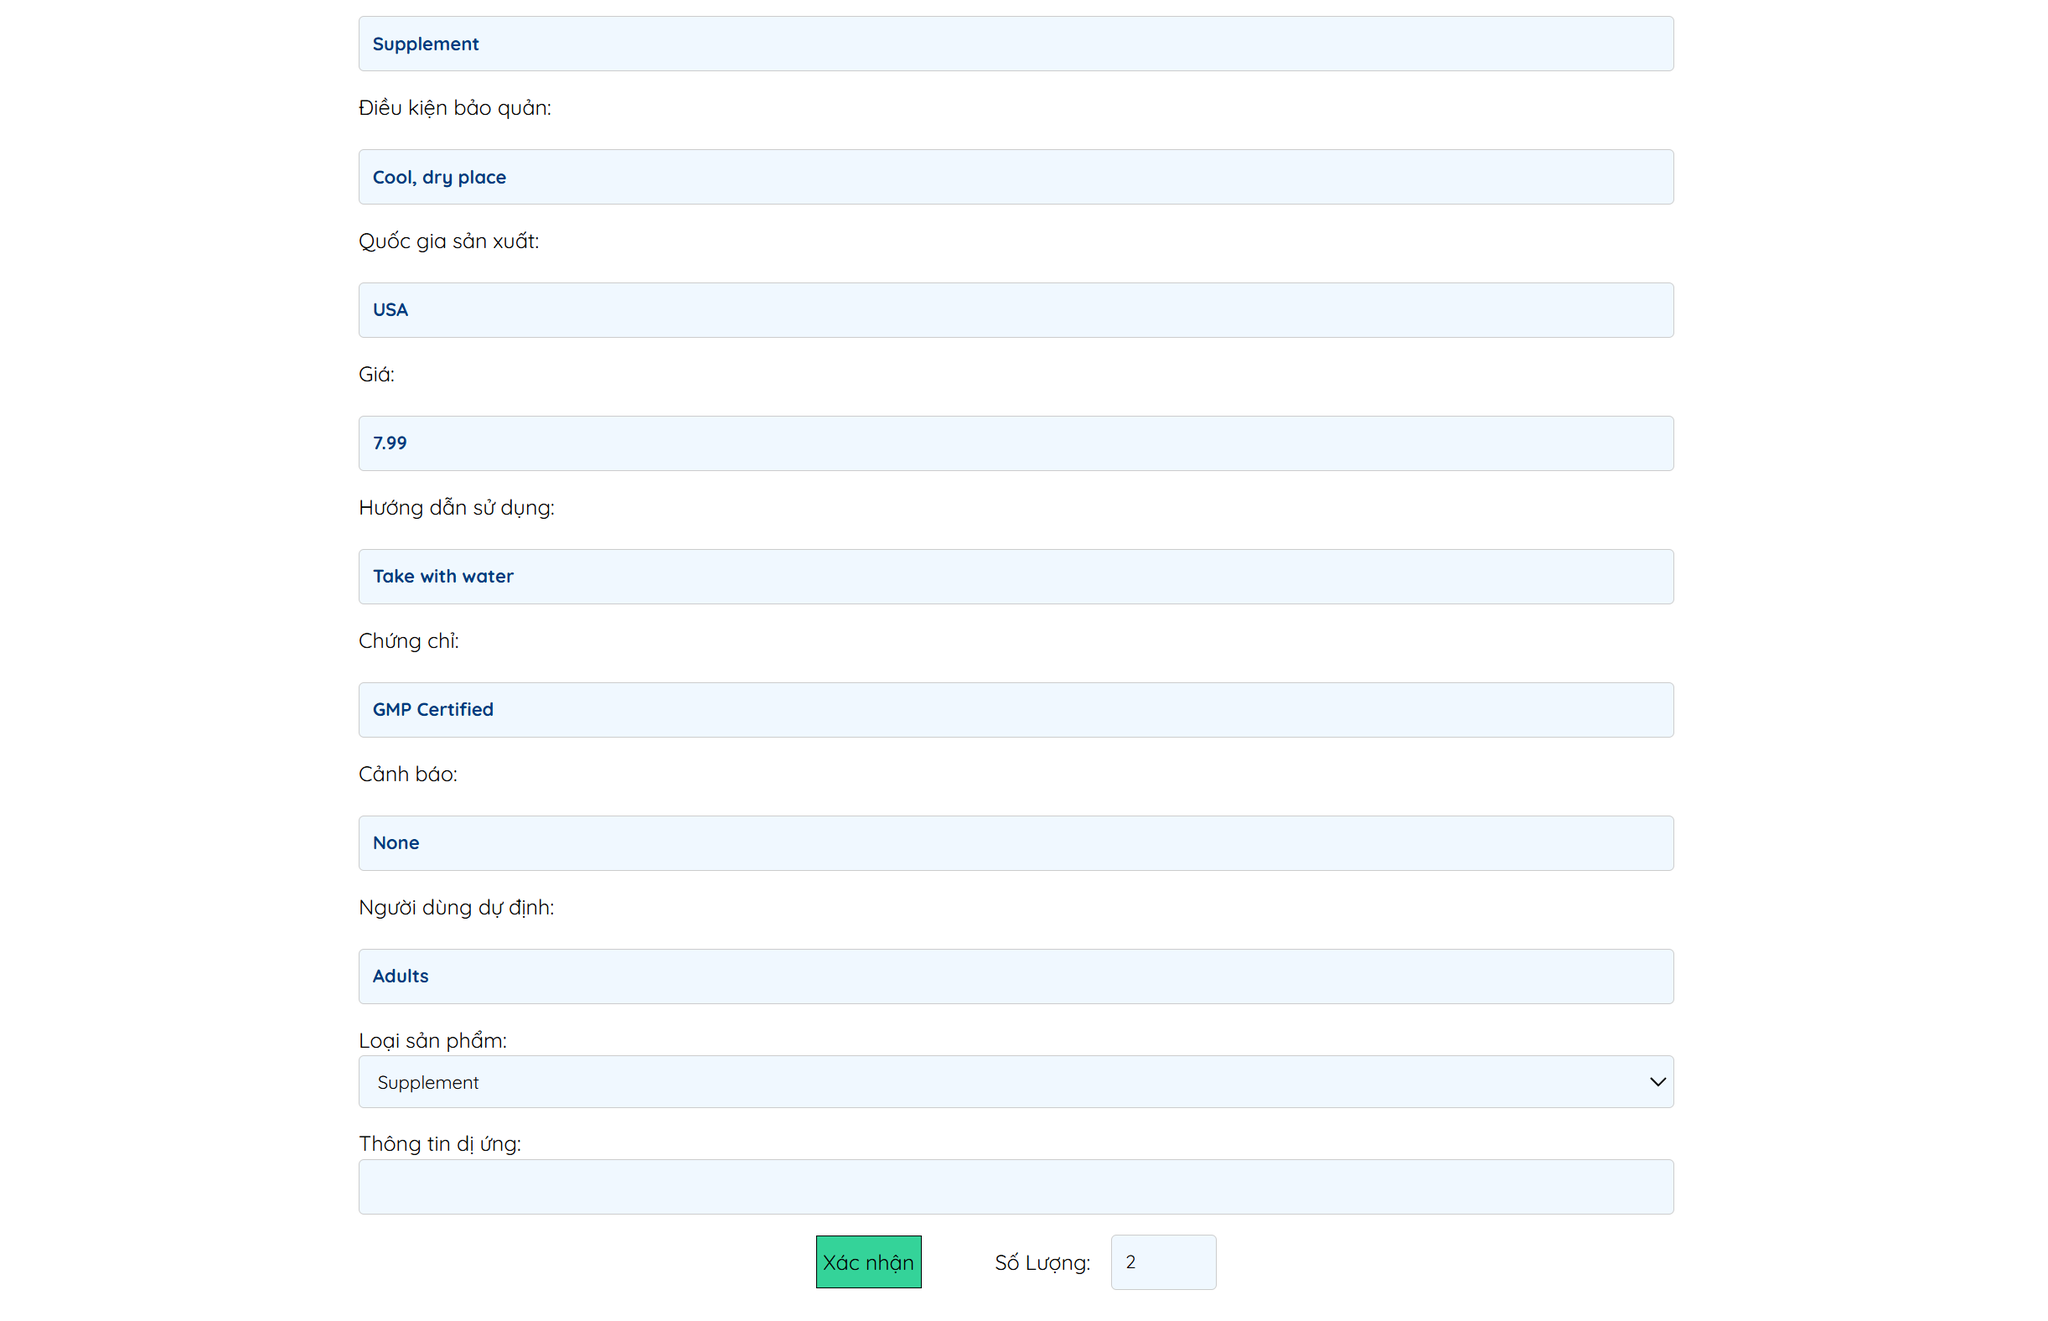
\includegraphics[scale=0.2]{Images/add_sp.png}
        \end{figure}
        
          \begin{figure}[H]  
        \hspace*{-3cm}     
            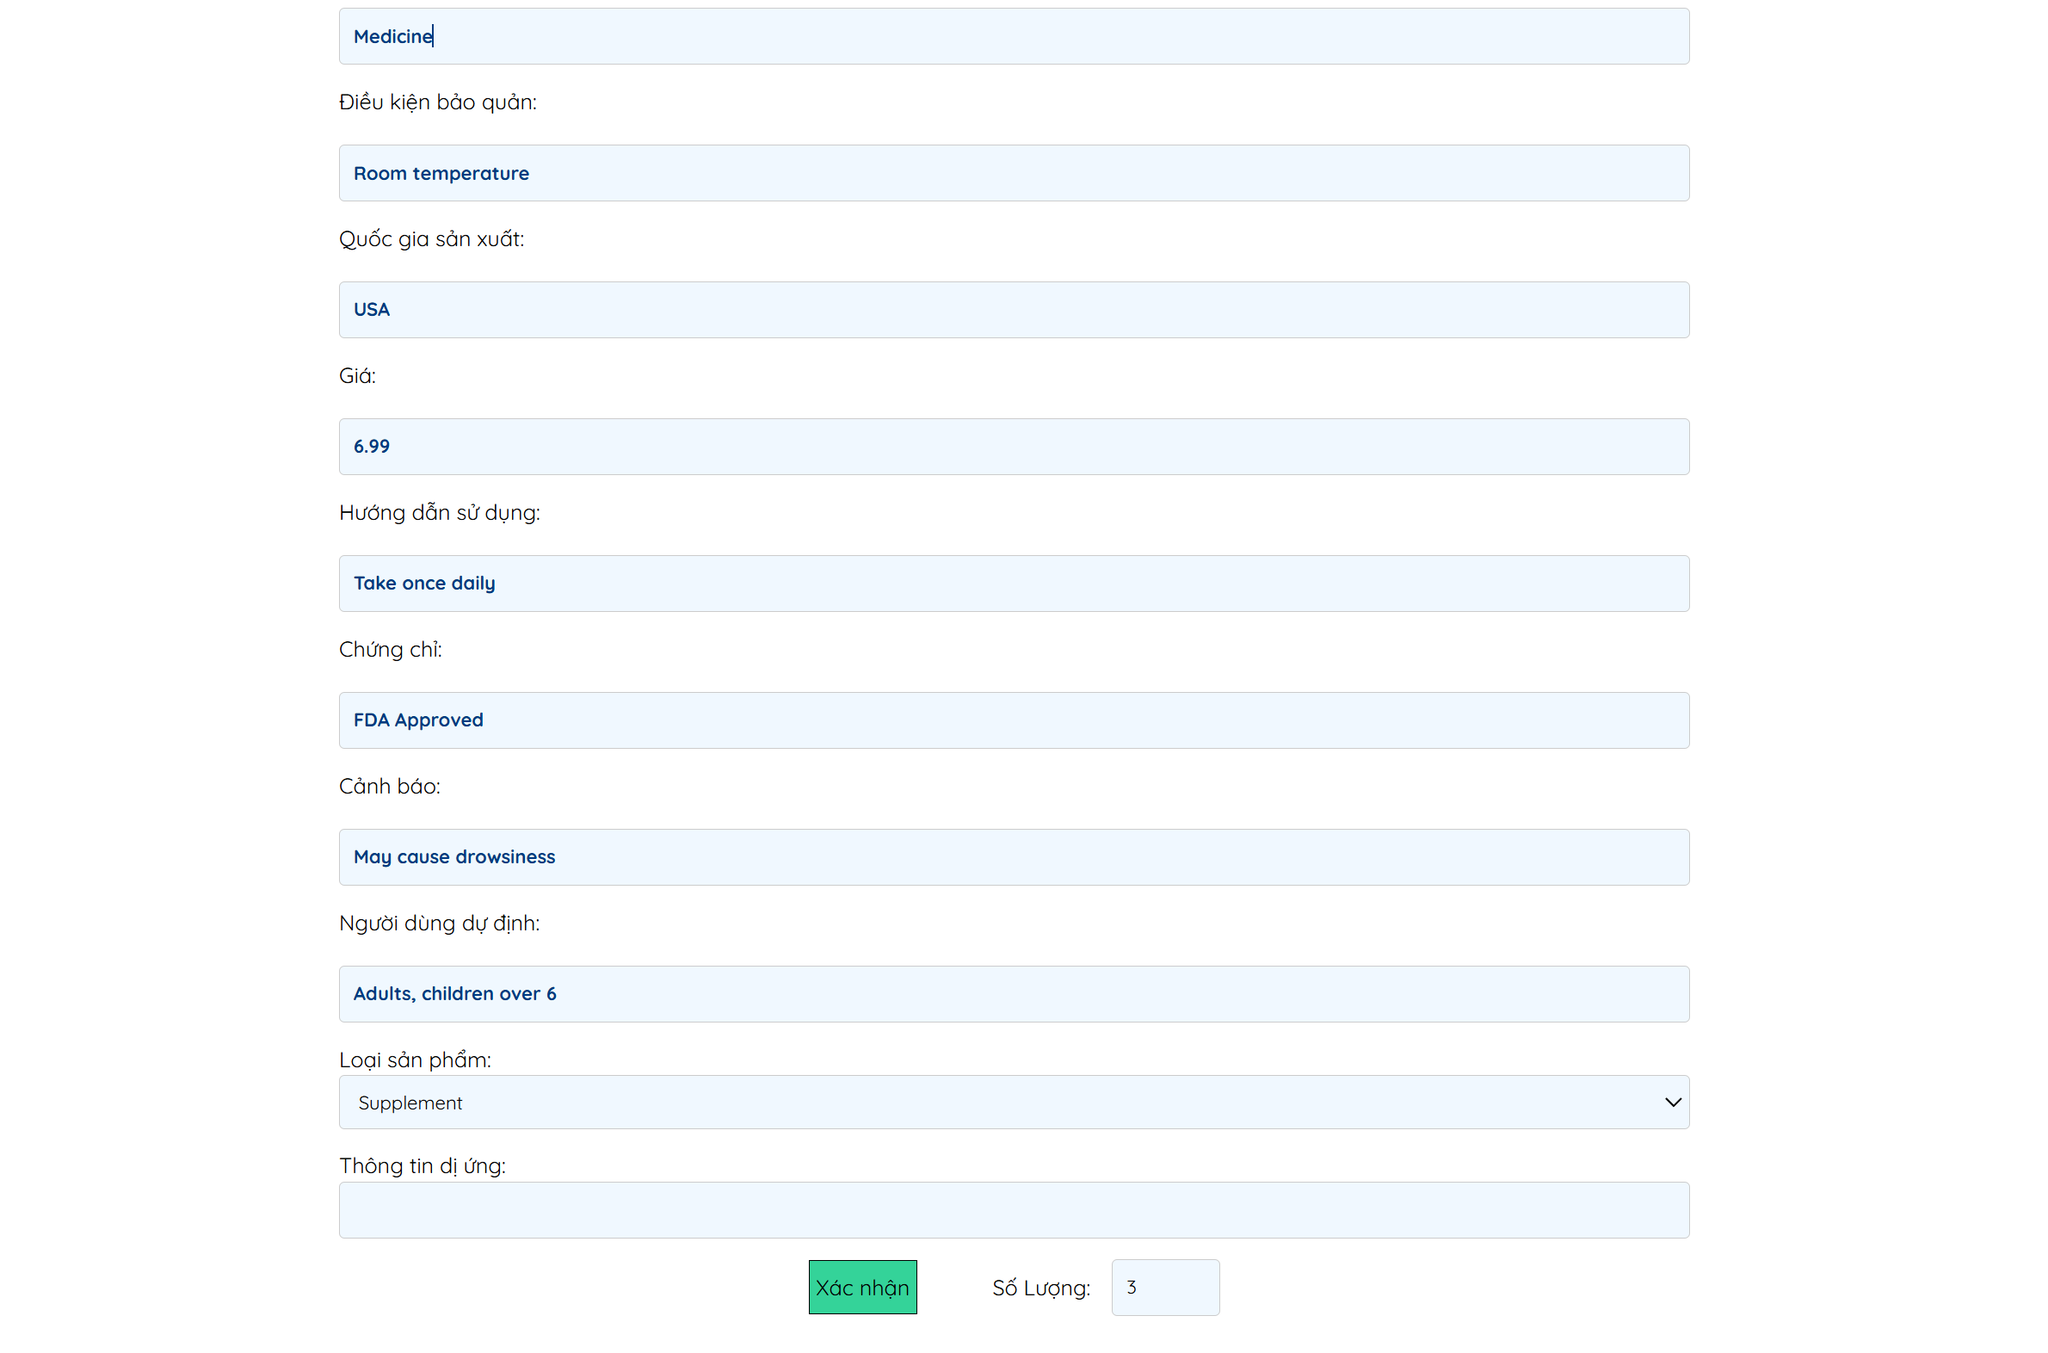
\includegraphics[scale=0.3]{Images/add_pro2.png}
        \end{figure}

         \begin{figure}[H]  
        \hspace*{-3cm}     
            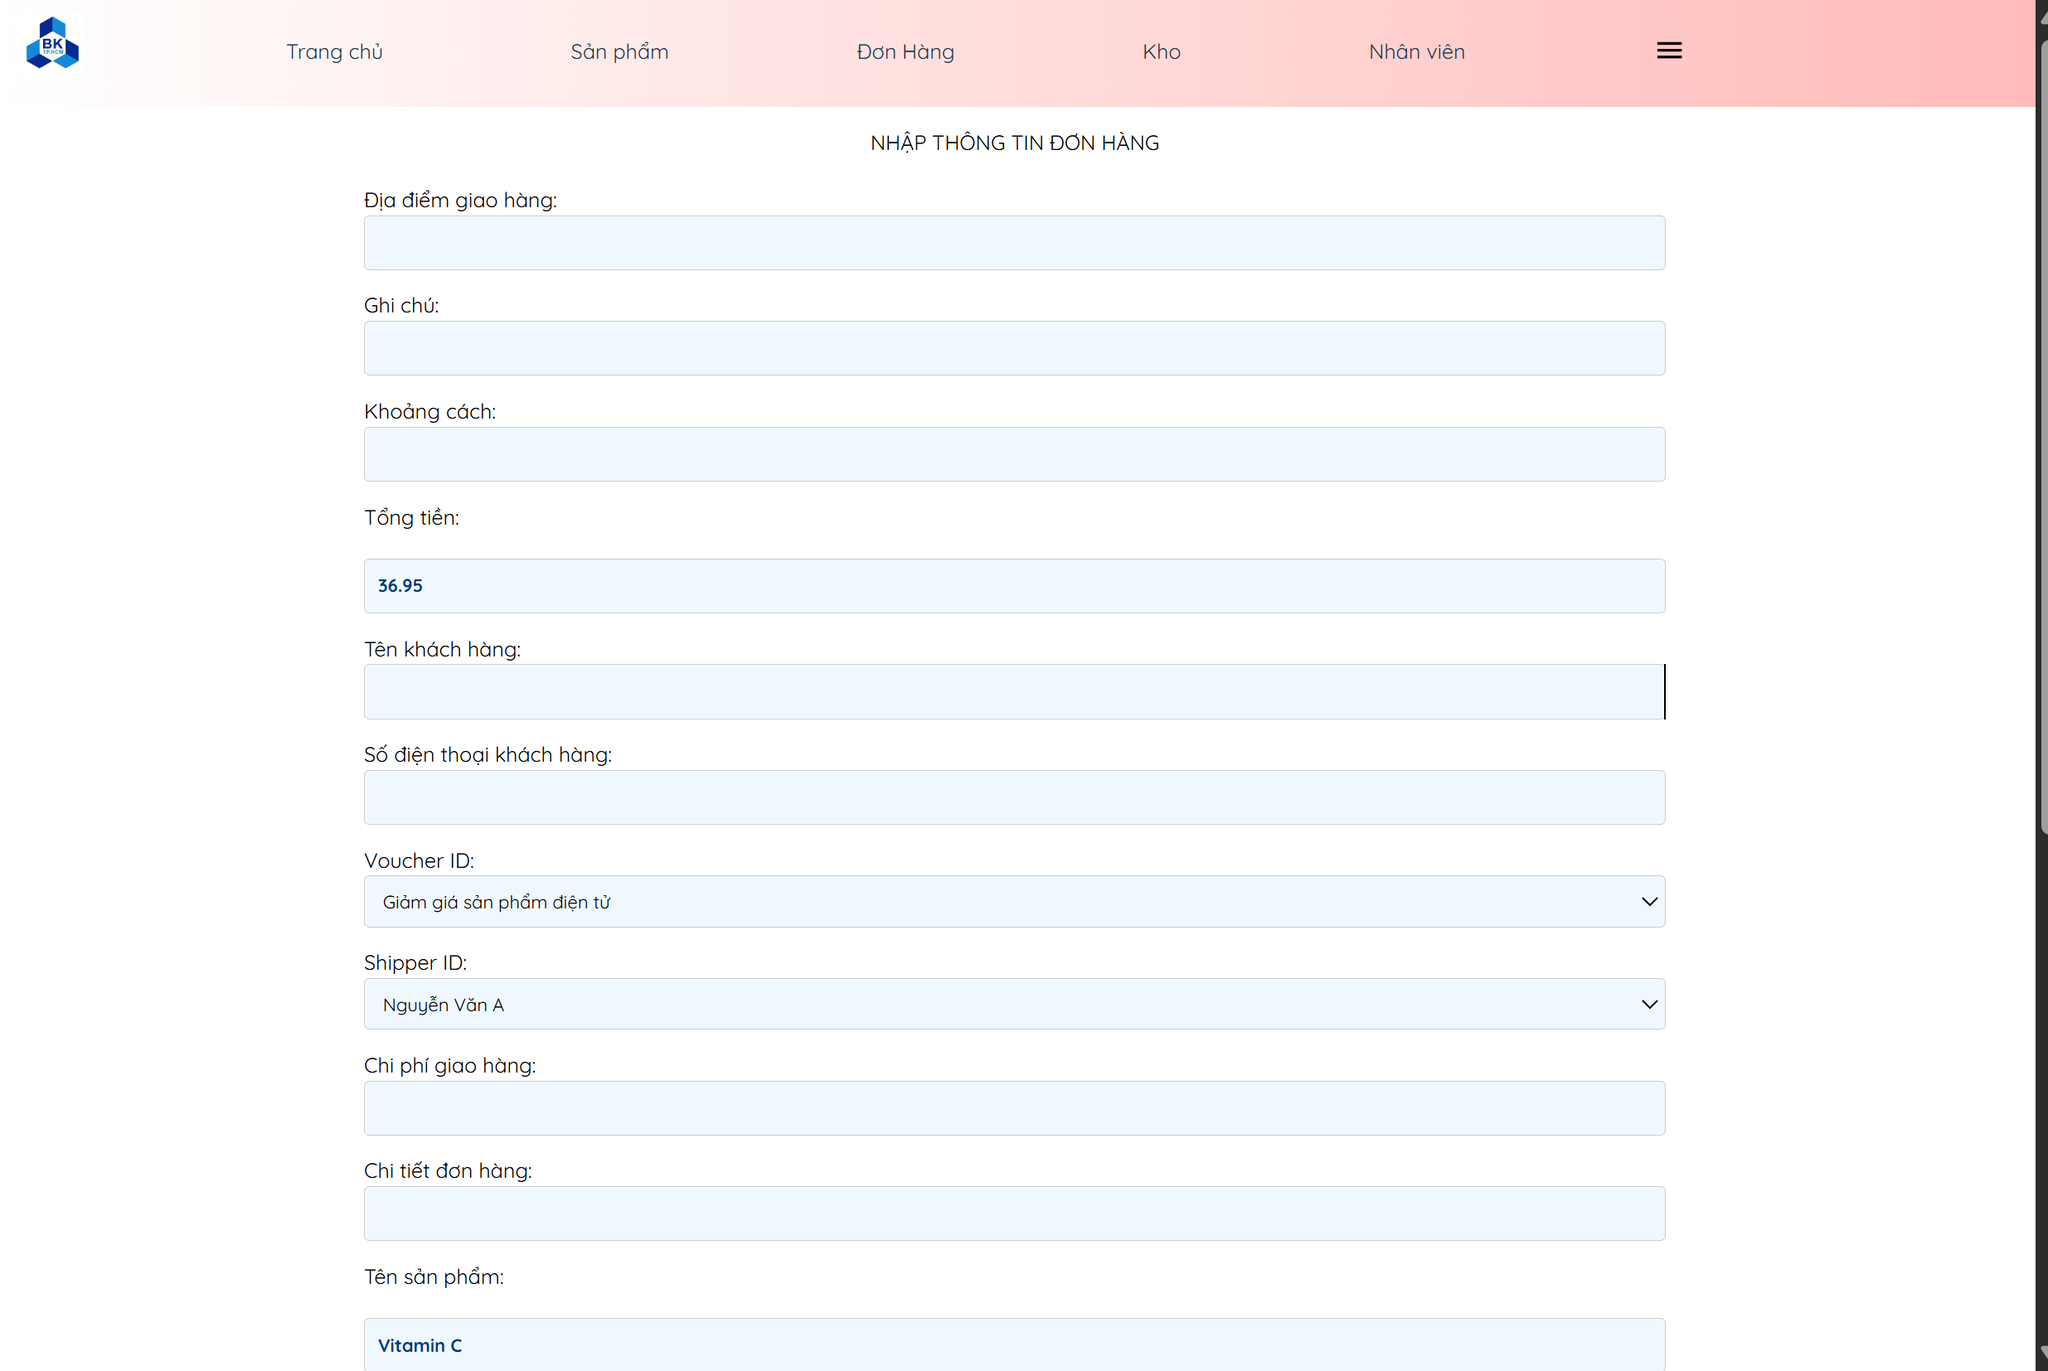
\includegraphics[scale=0.26]{Images/insertDon1.png}
        \end{figure}

         \begin{figure}[H]  
        \hspace*{-3cm}     
            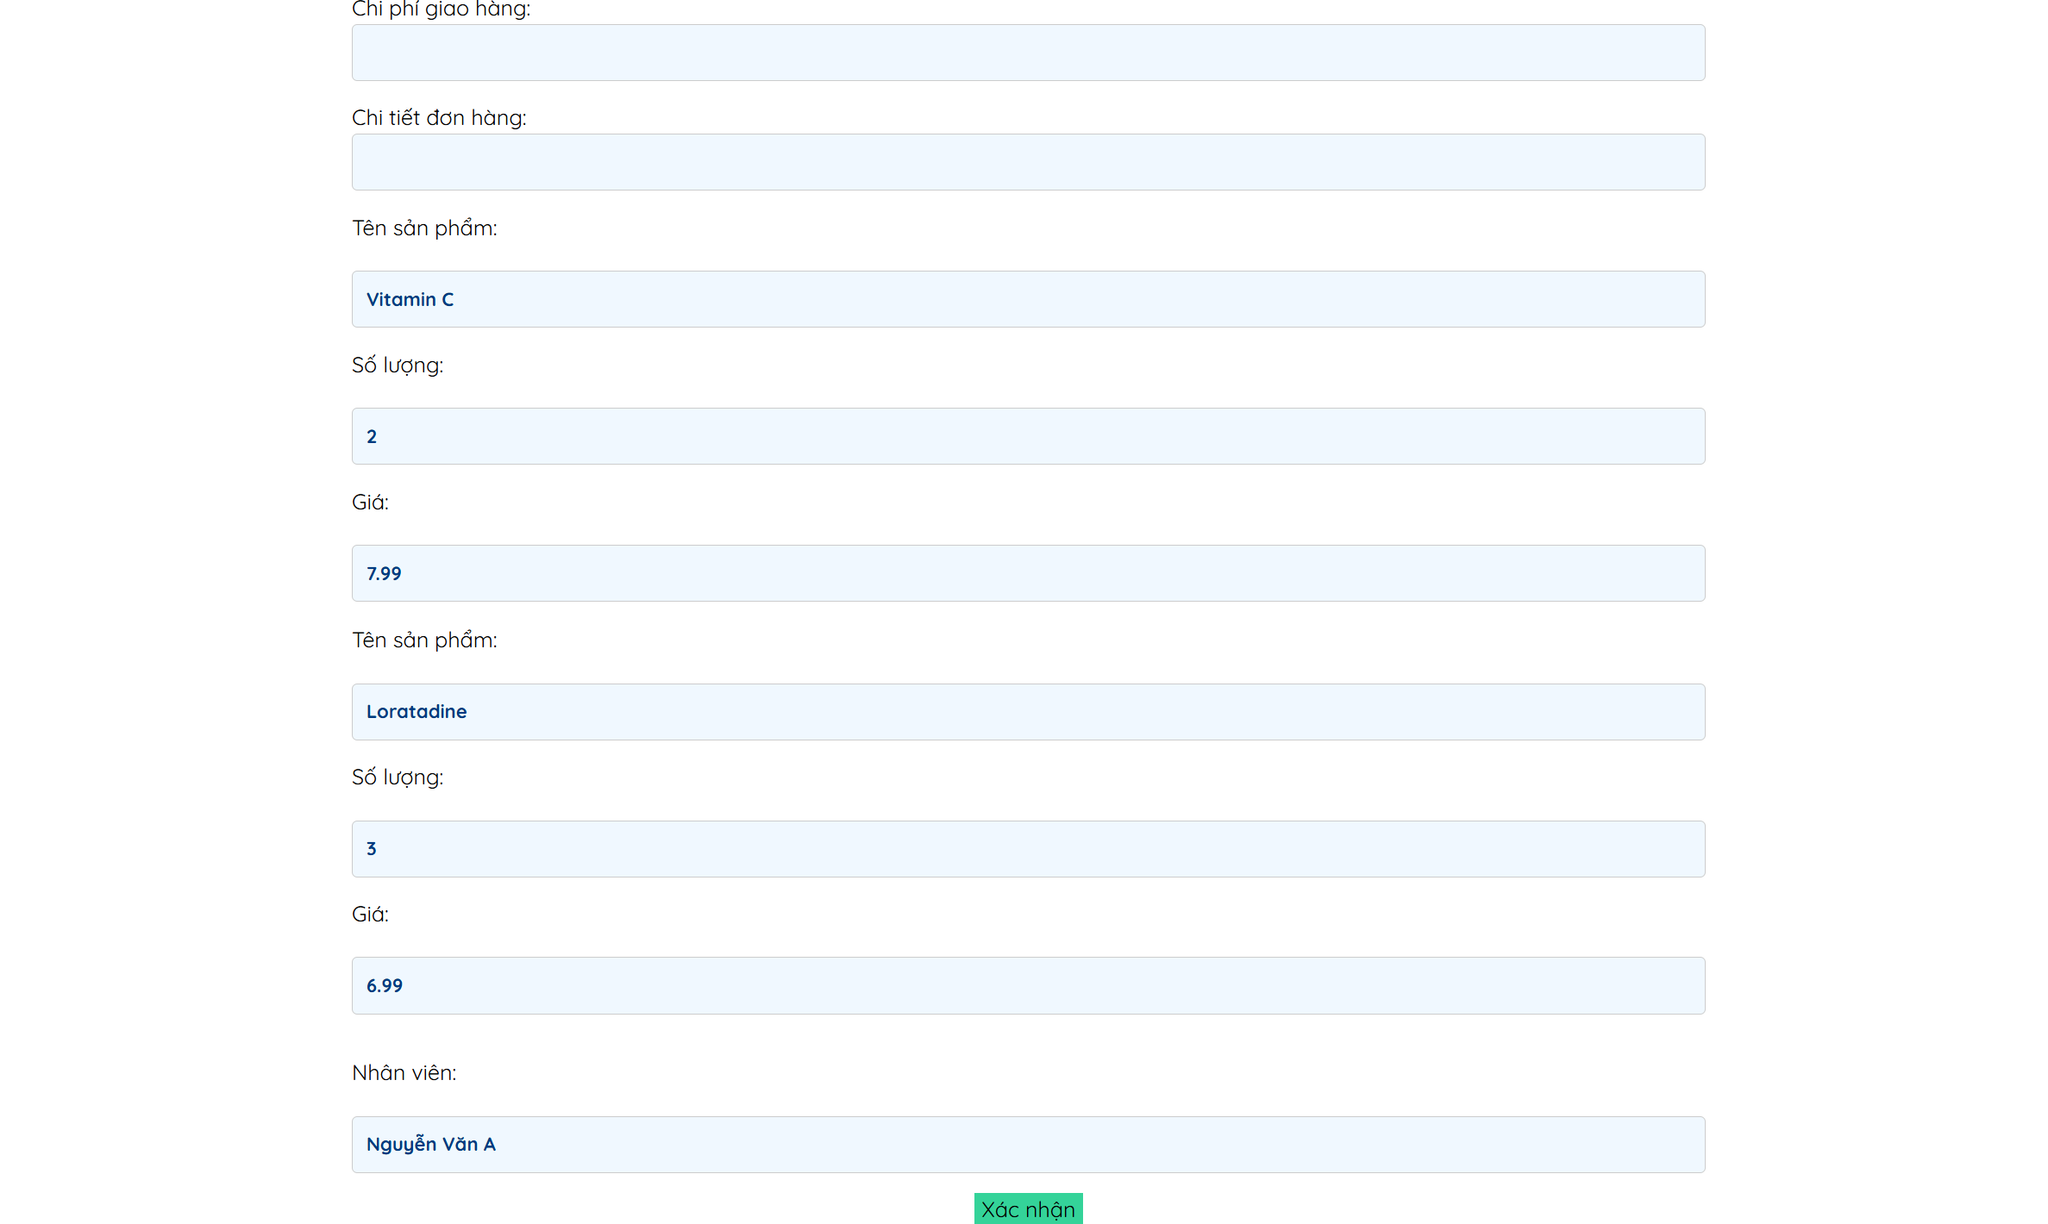
\includegraphics[scale=0.3]{Images/insertPhar2.png}
        \end{figure}

            \begin{figure}[H]  
        \hspace*{-3cm}     
            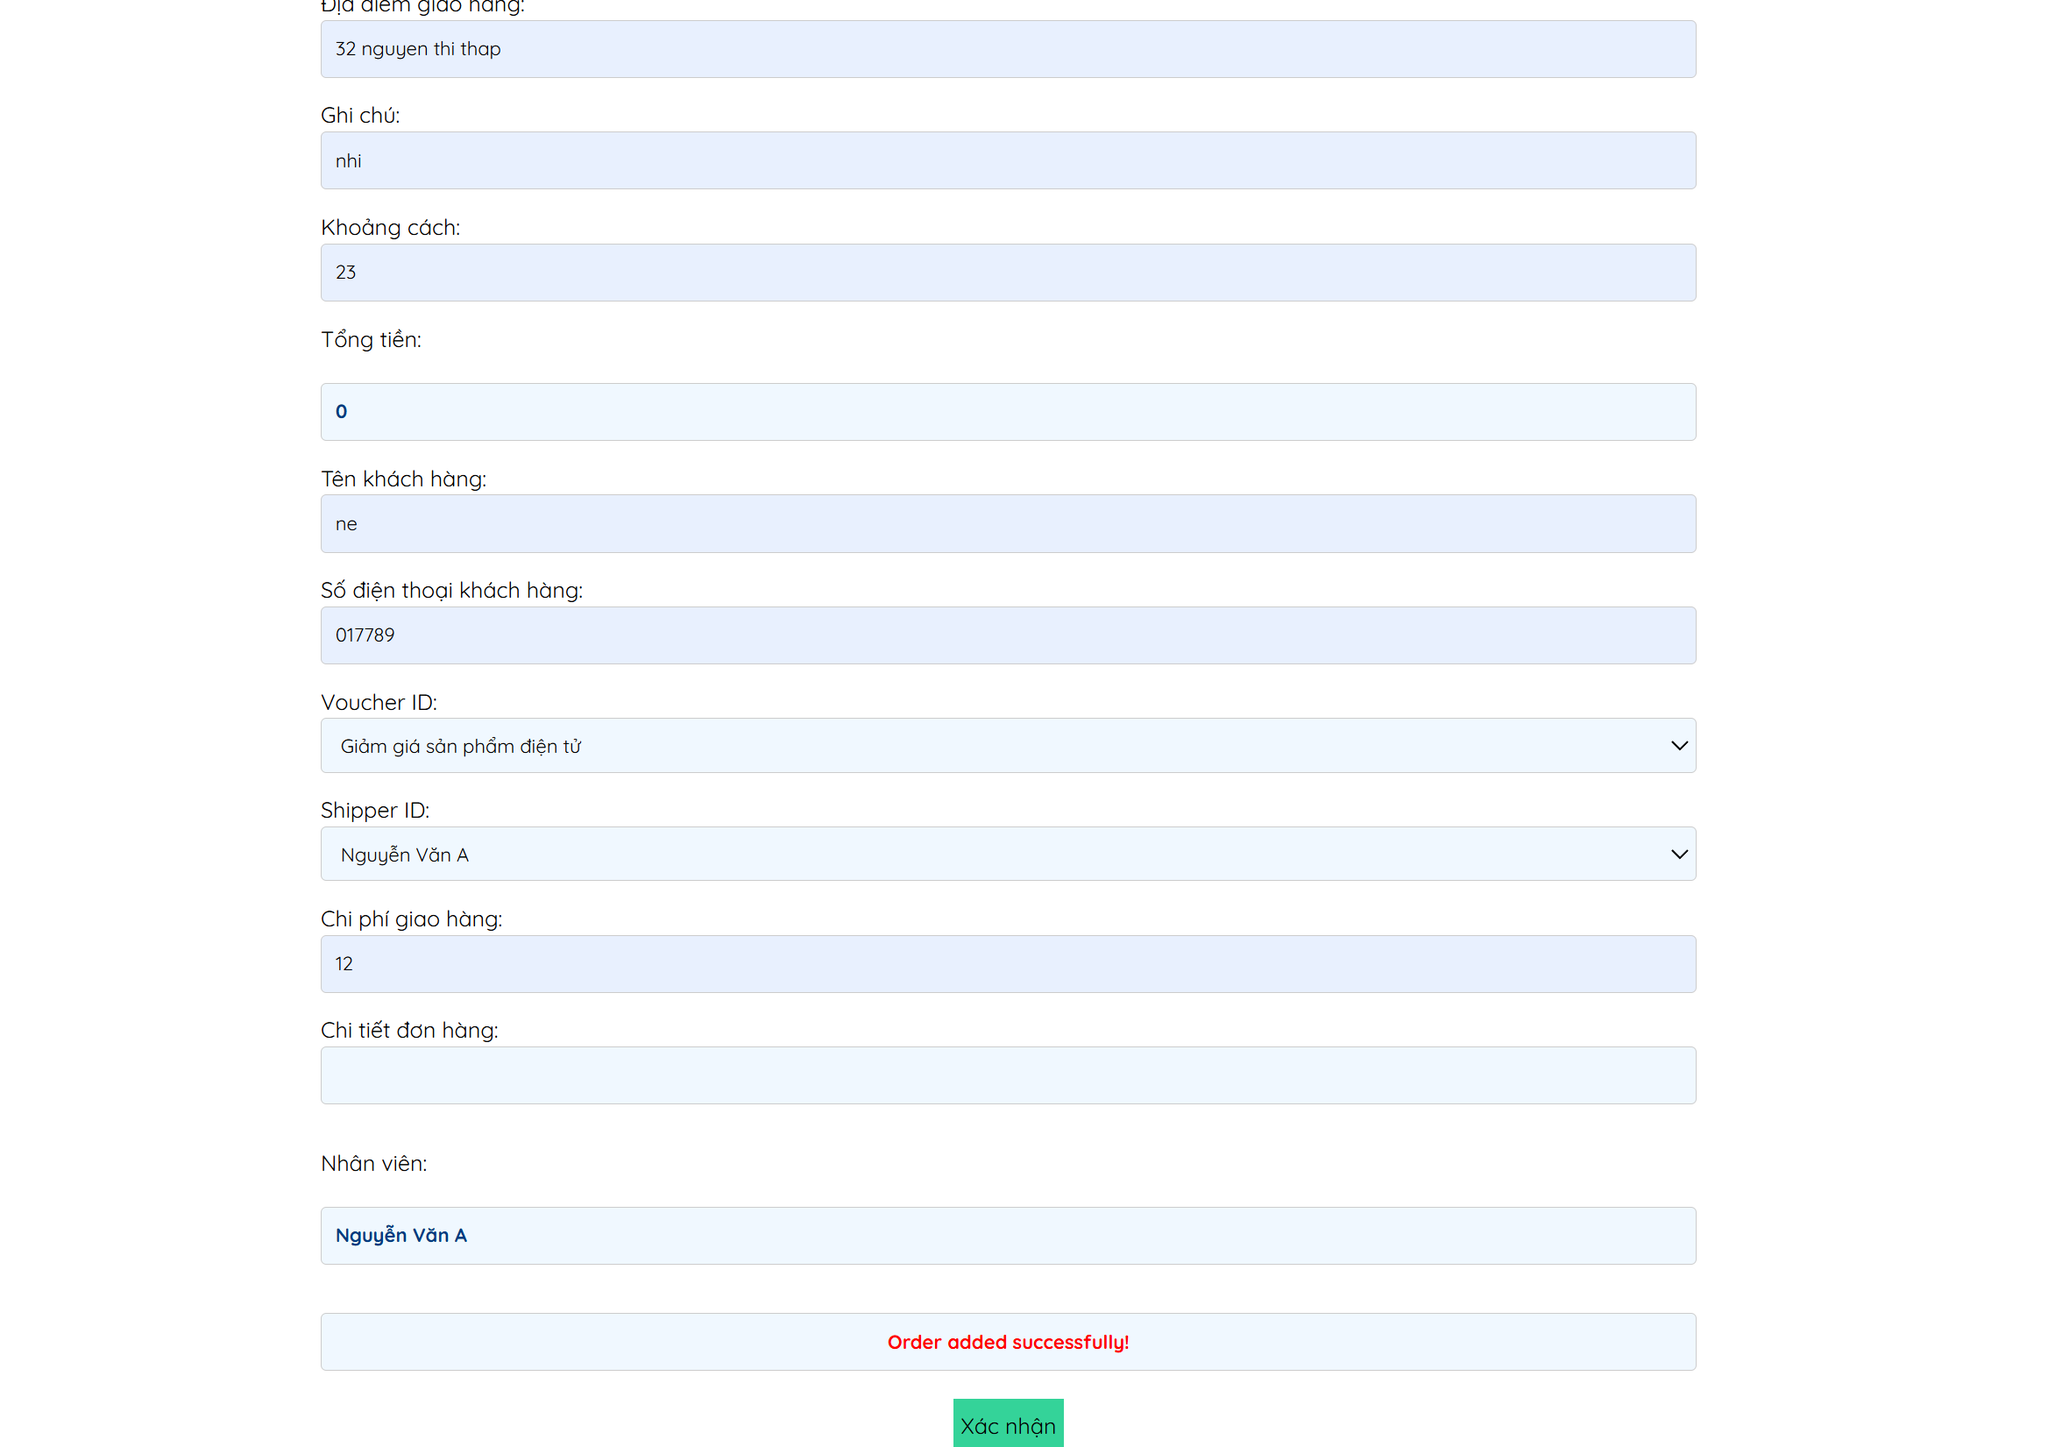
\includegraphics[scale=0.3]{Images/insertPharmaSucc.png}
        \end{figure}

        


        

\subsection{Sản phẩm}
Người dùng có thể xem thông tin chi tiết của các sản phẩm có trong kho và có thể thêm sản phẩm vào kho.
\begin{figure}[H]
\hspace*{-1cm}     
    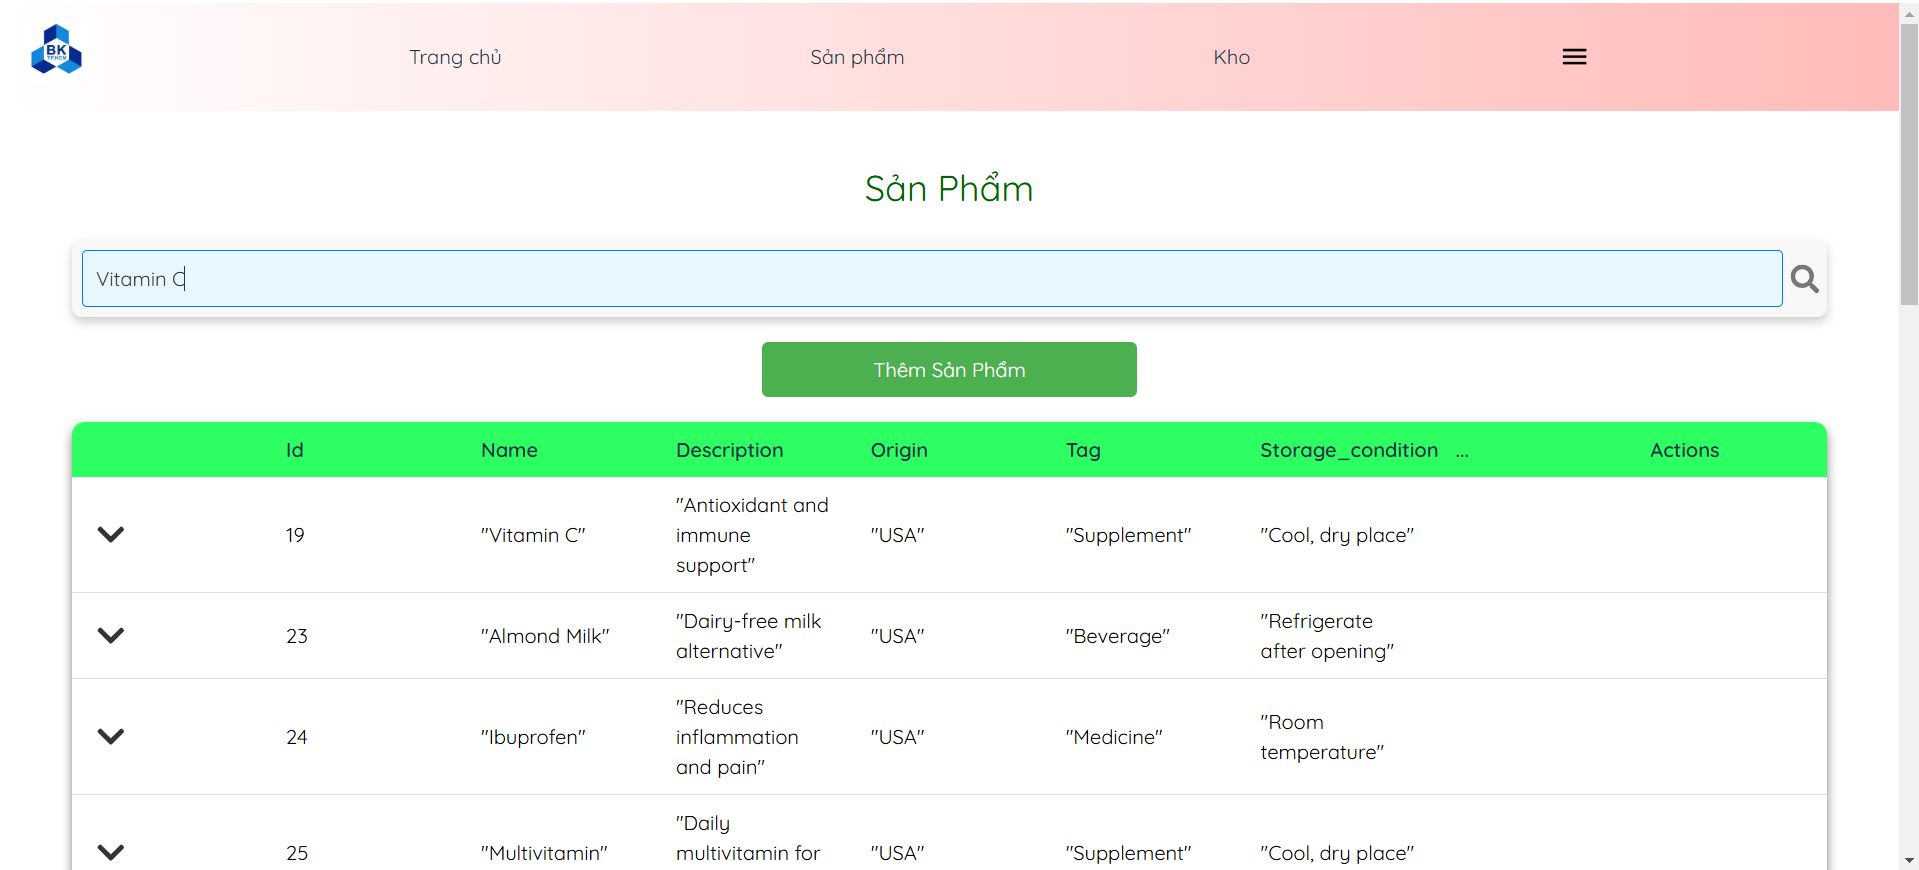
\includegraphics[scale=0.3]{Images/products_page/a1 (1).png}

\hspace*{-1cm}   
    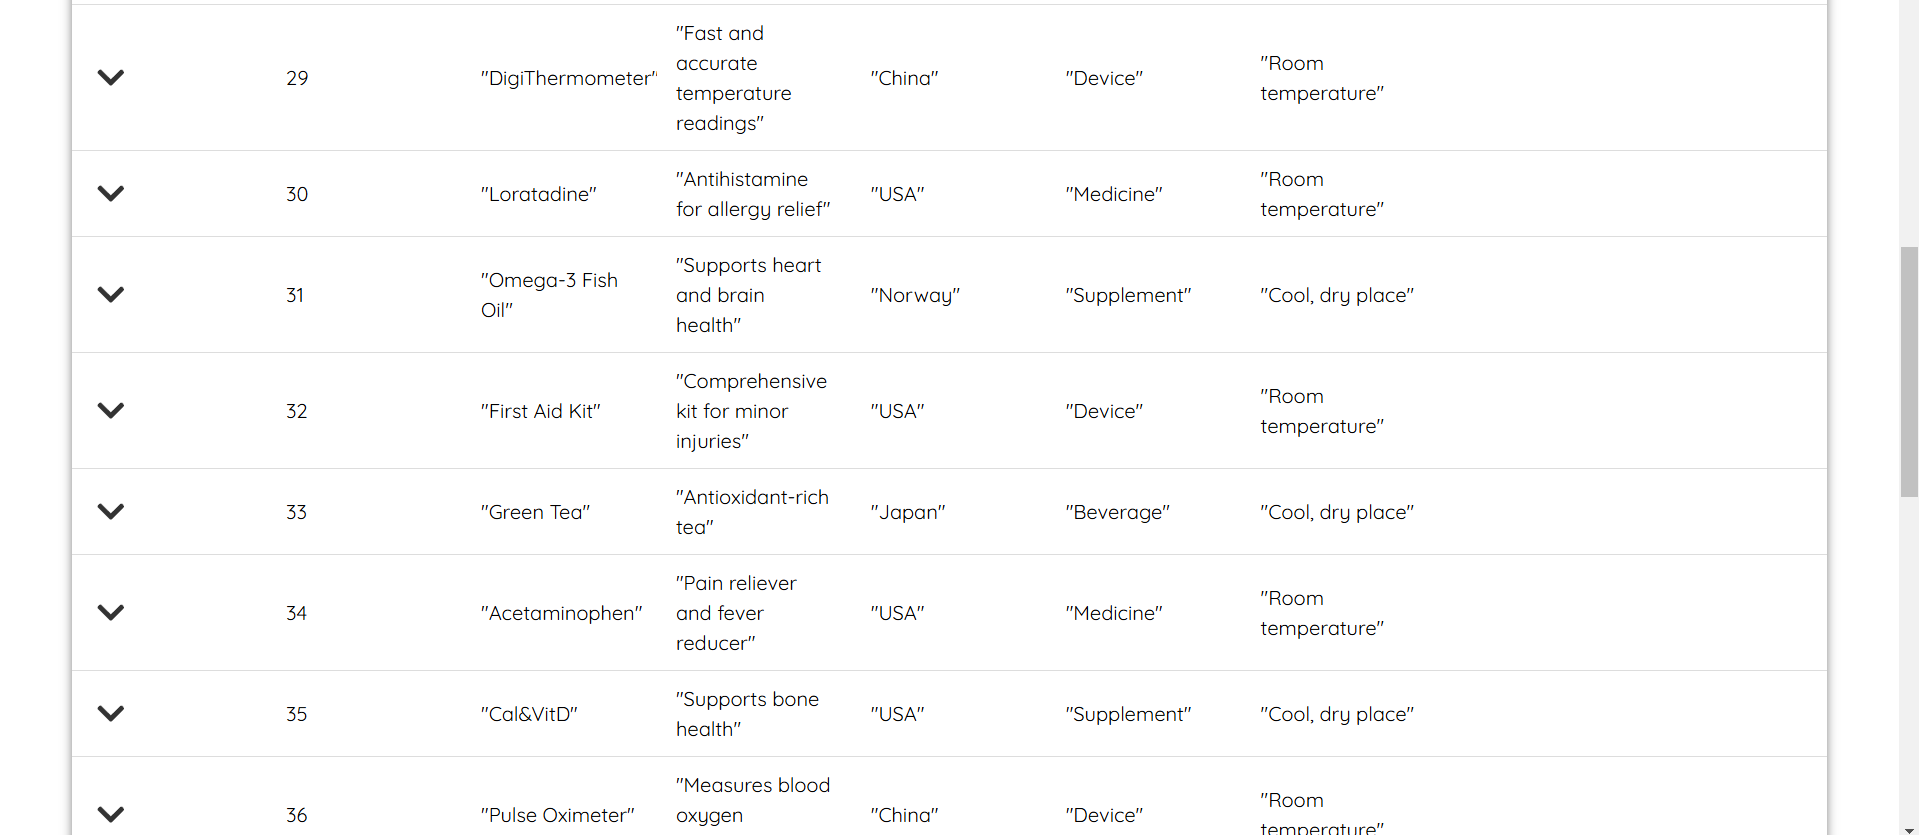
\includegraphics[scale=0.3]{Images/products_page/a1 (2).png}
\end{figure}


    \begin{figure}[H]
\hspace*{-2cm}   
%  \centering
    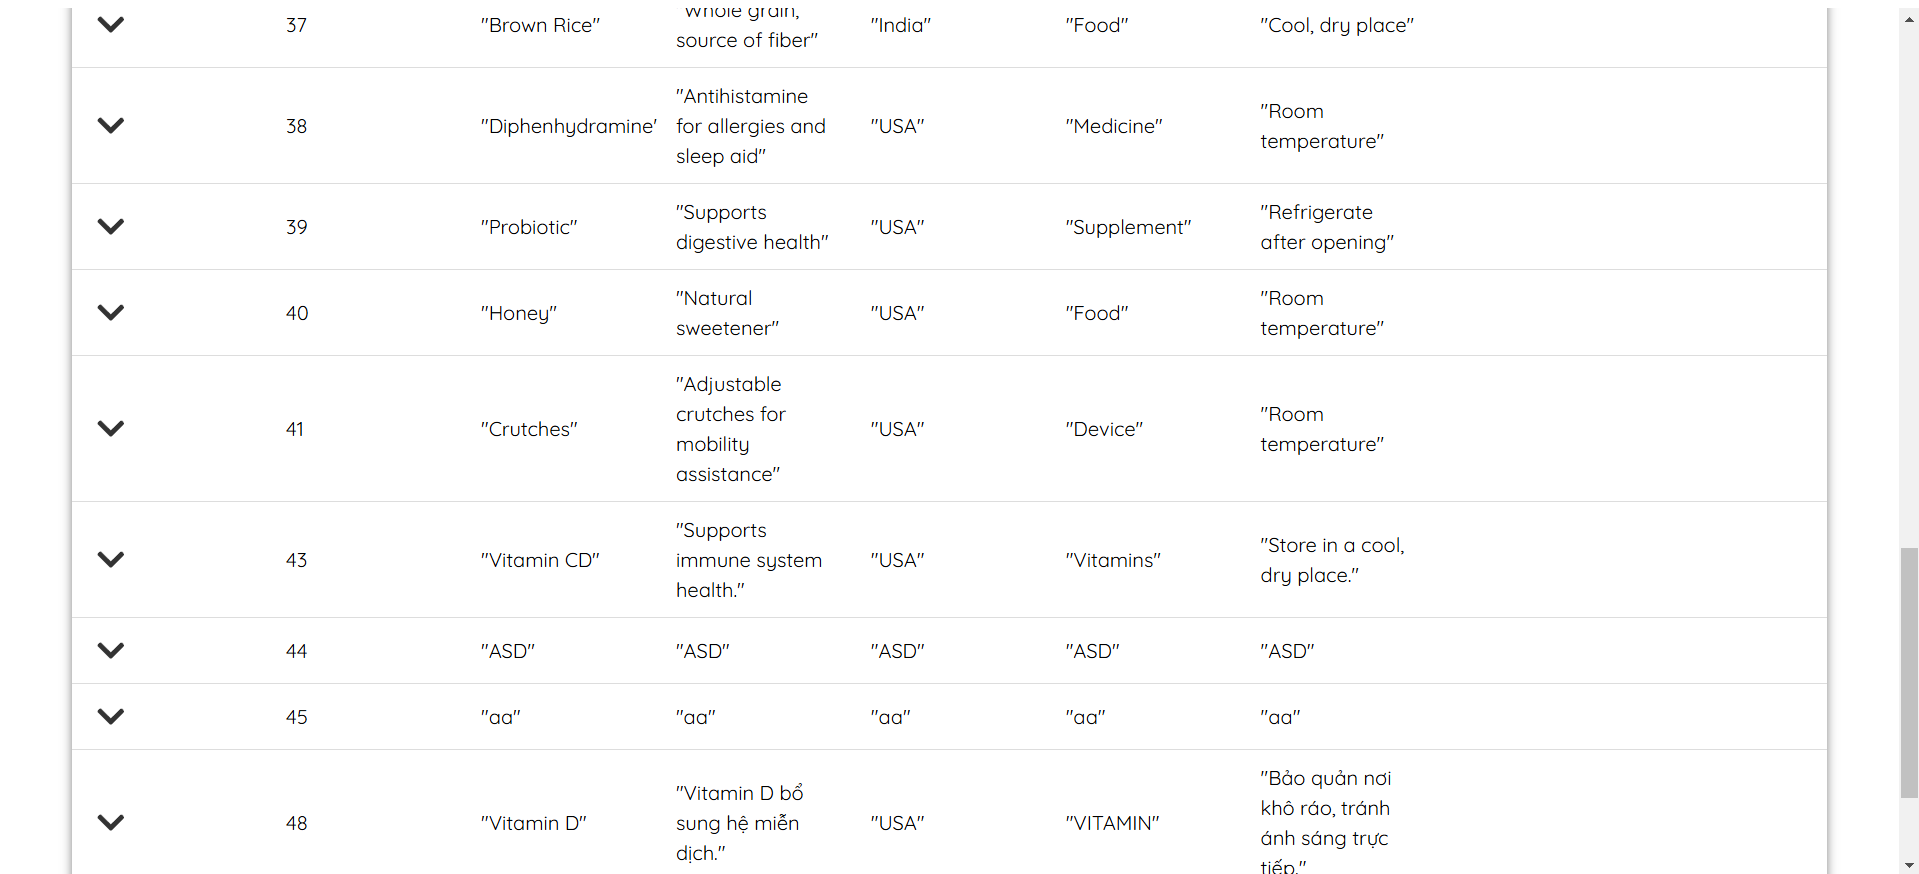
\includegraphics[scale=0.3]{Images/products_page/a1 (3).png}


\hspace*{-2cm}        
    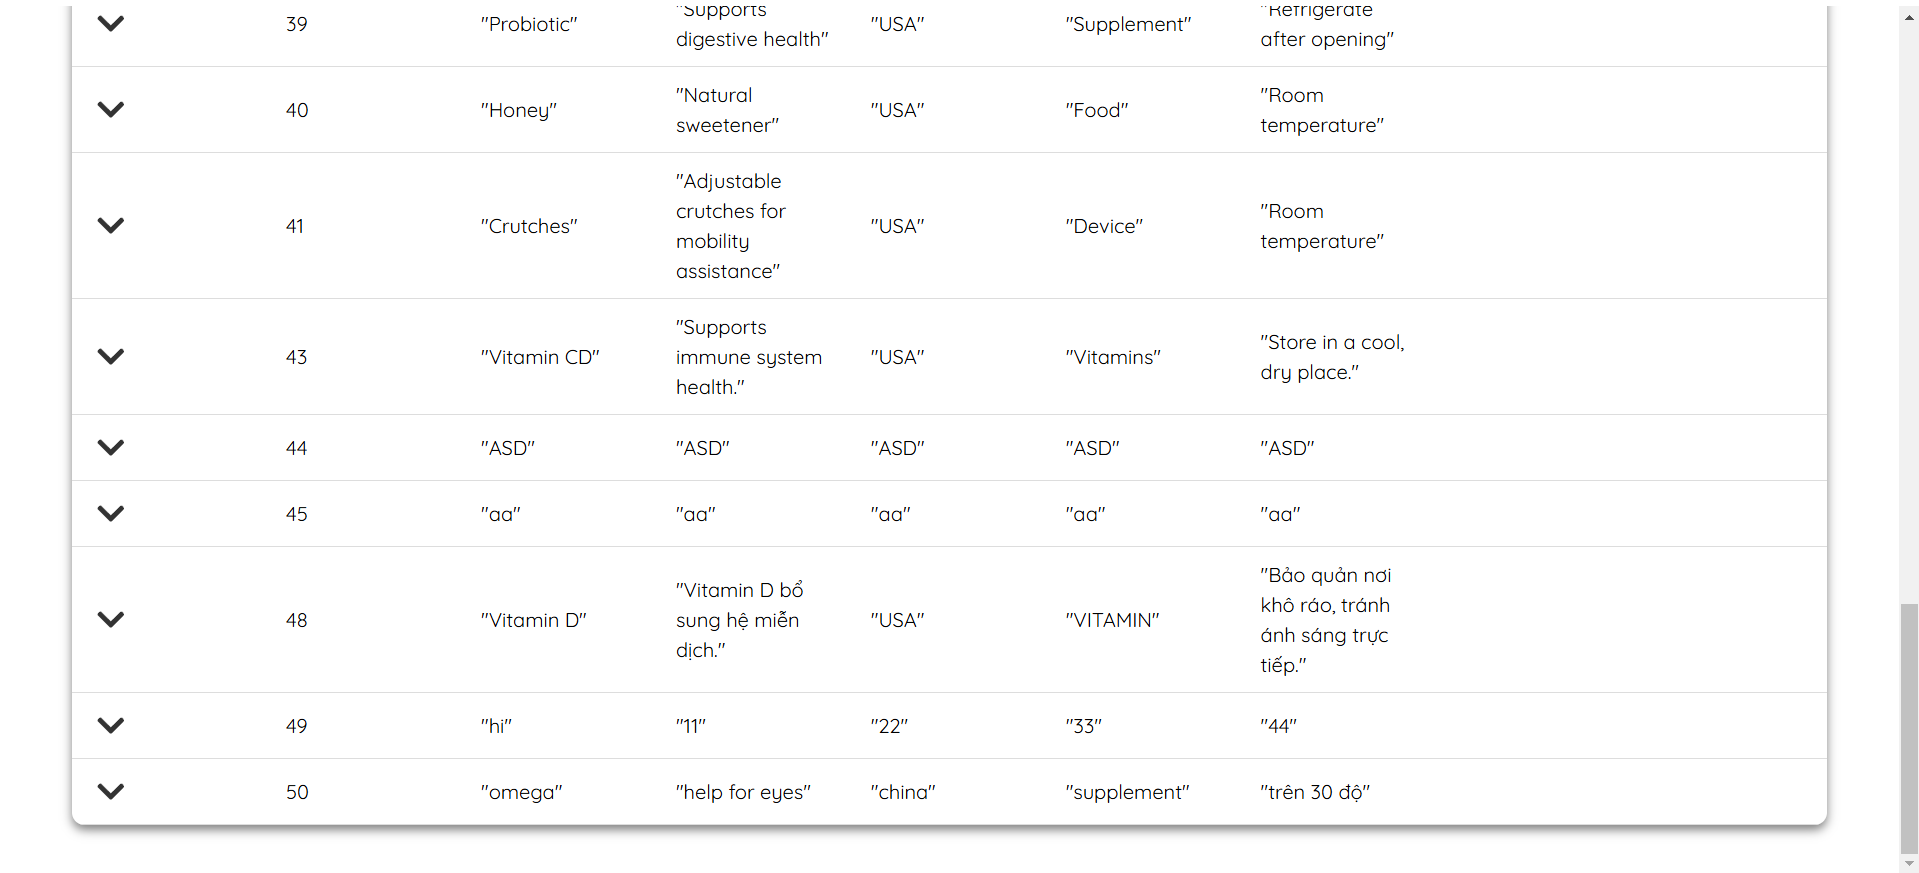
\includegraphics[scale=0.3]{Images/products_page/a1 (4).png}
    \caption{Màn hình xem các sản phẩm}
\end{figure}

\begin{figure}[H]

\hspace*{-1cm}        
    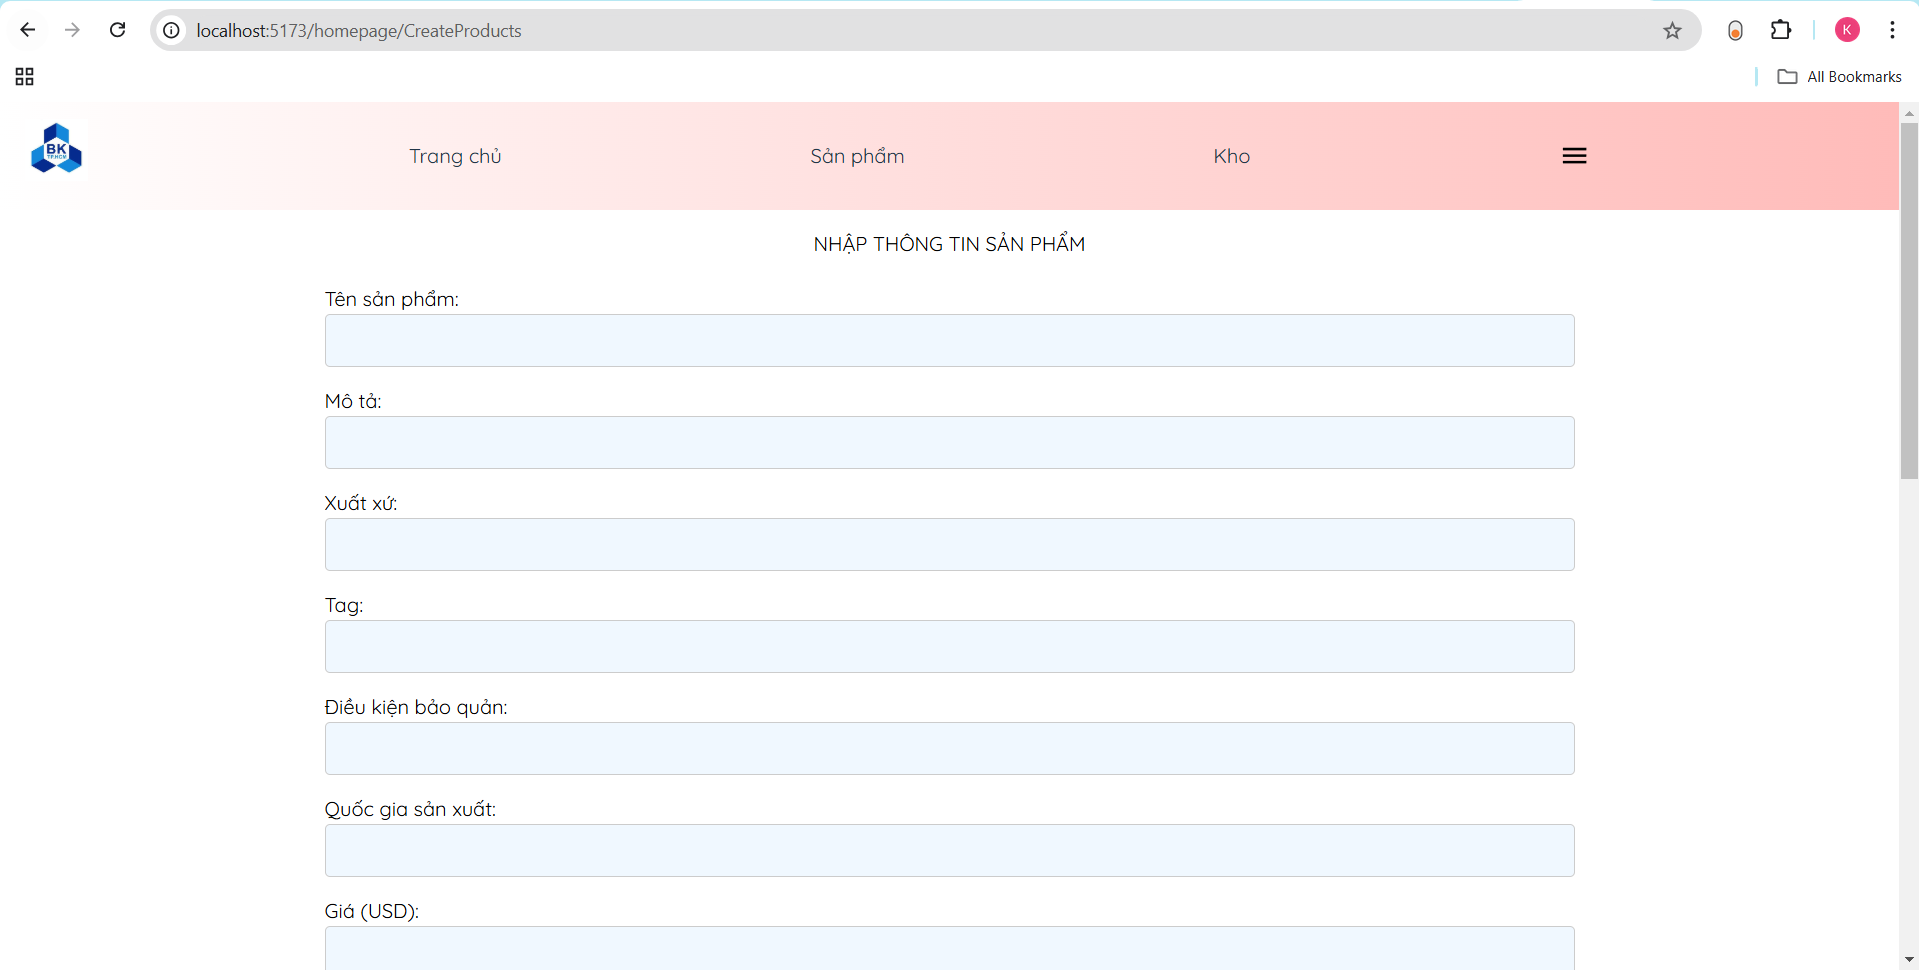
\includegraphics[scale=0.3]{Images/products_page/b1 (1).png}
    % \caption{Màn hình xem các sản phẩm}
\end{figure}

\begin{figure}[H]
\hspace*{-1cm}   
    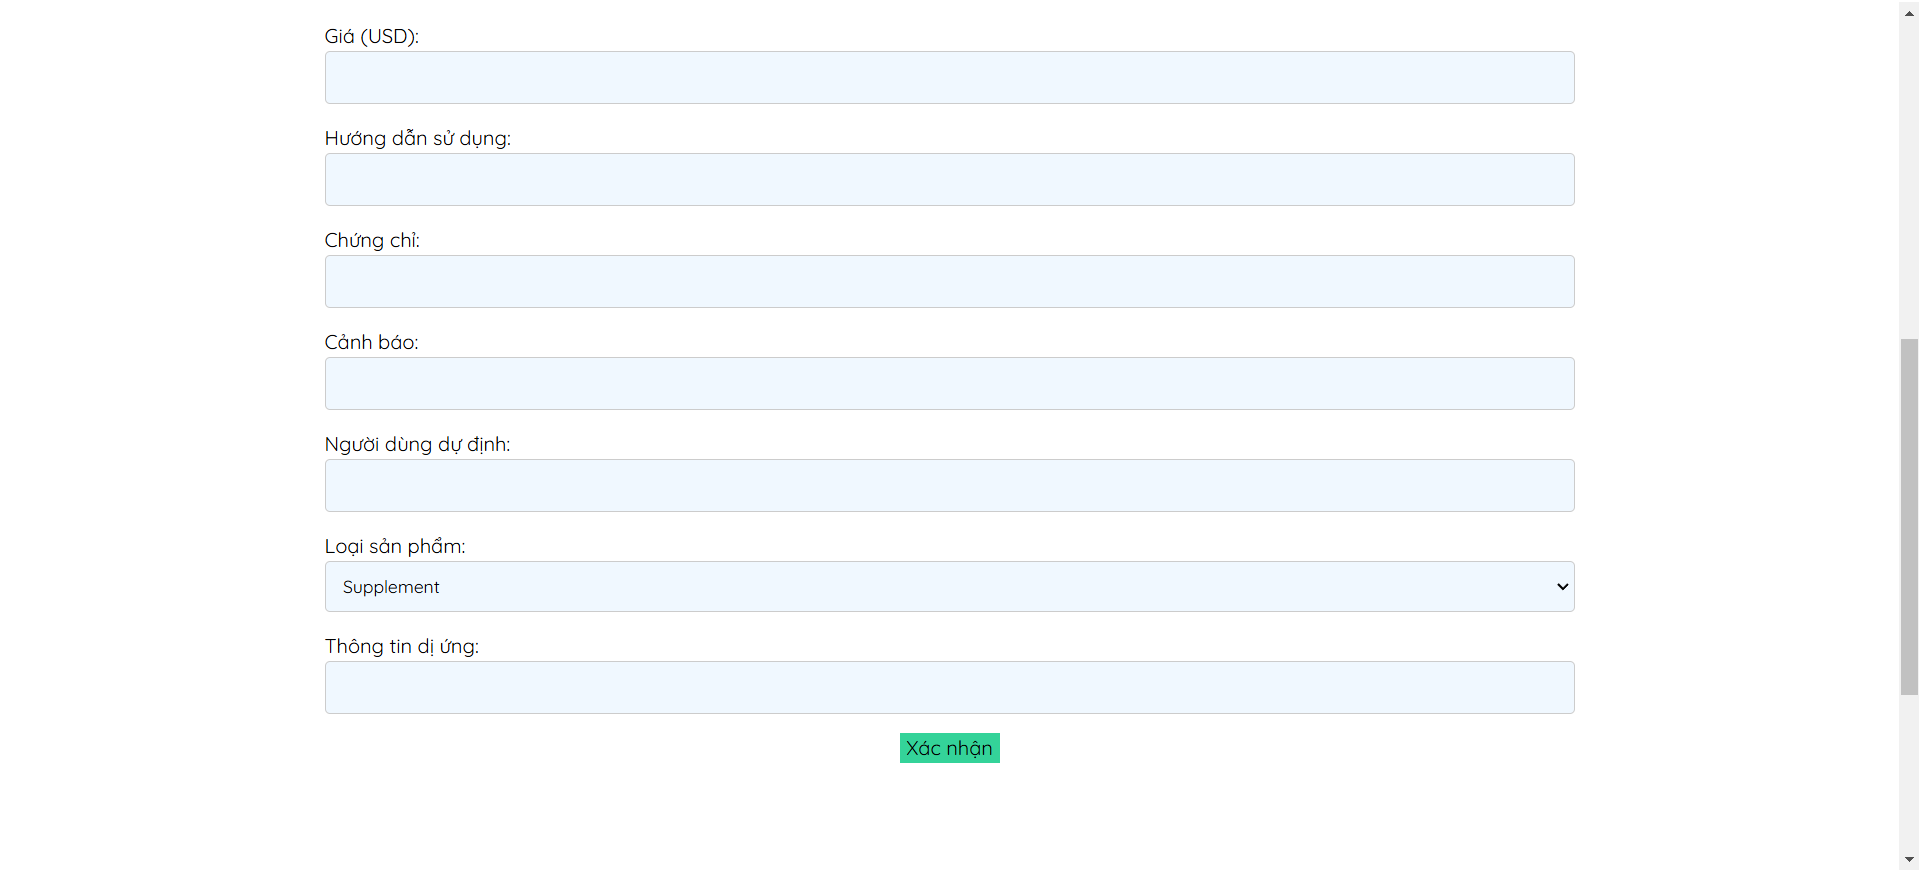
\includegraphics[scale=0.3]{Images/products_page/b1 (2).png}
    \caption{Màn hình thêm sản phẩm}
    
\end{figure}

Ngoài ra, ở phần "Thêm sản phẩm" để hạn chế người dùng nhập sai thông tin, có giới hạn độ dài của "Tên sản phẩm" và "Quốc gia sản xuất" không được quá 16 ký tự.

\begin{figure}[H]
    \hspace*{-2cm}   
        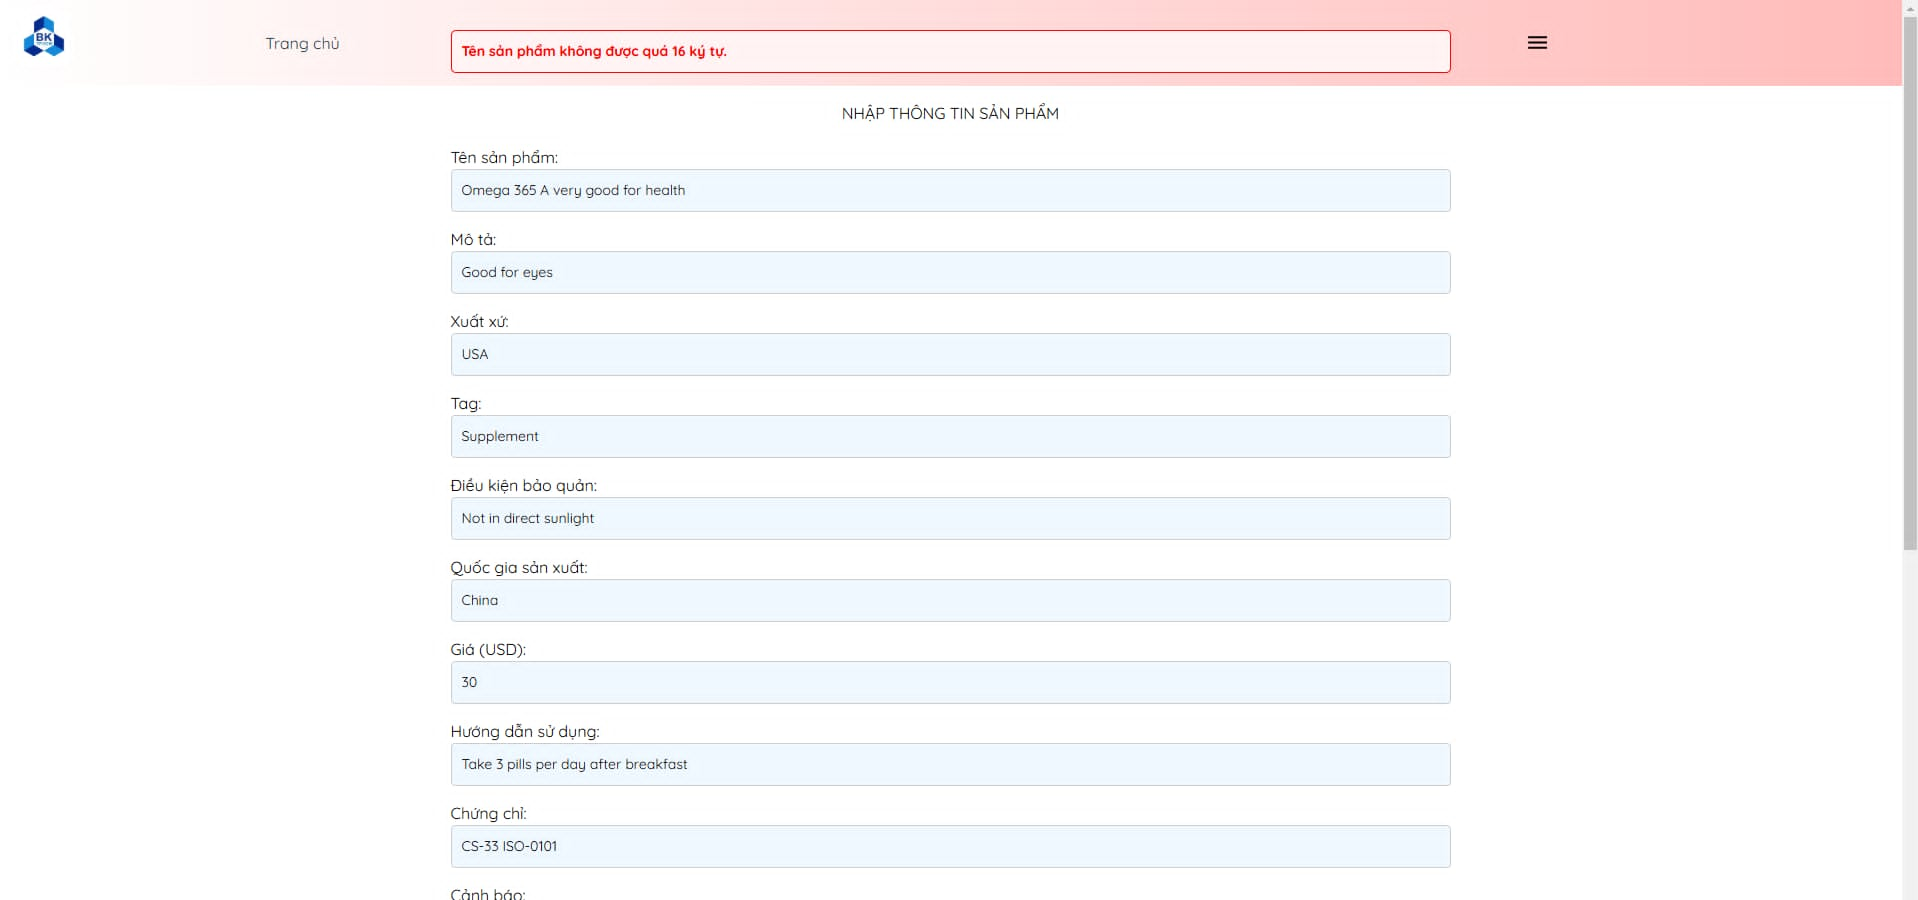
\includegraphics[scale=0.26]{Images/products_page/prod_demo_01.jpg}
    \hspace*{-2cm}   
        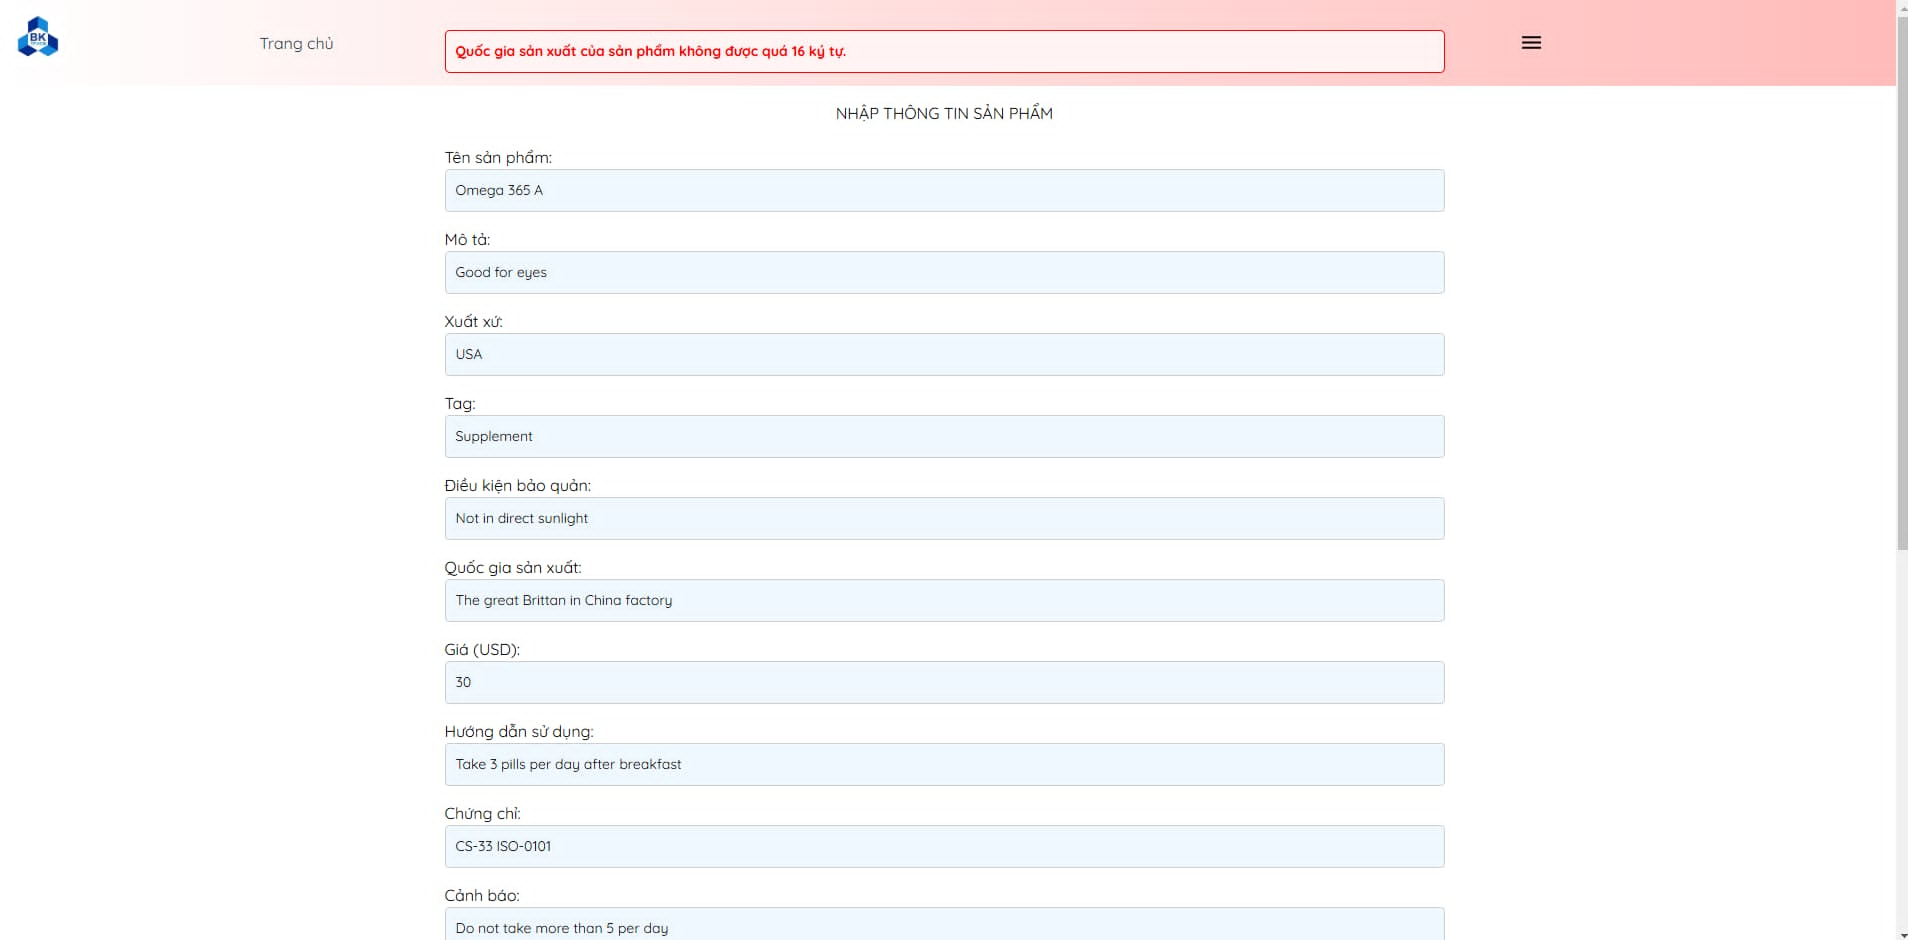
\includegraphics[scale=0.26]{Images/products_page/prod_demo_02.jpg}
        \caption{Giới hạn độ dài trong phần "Thêm sản phẩm"}
        
\end{figure}

\subsection{Kho hàng và lô hàng}
Người dùng có thể xem các lô hàng hiện có trong kho hàng và tiến hành thêm lô hàng nếu muốn.
\begin{figure}[h!]
\hspace*{-1cm}   
    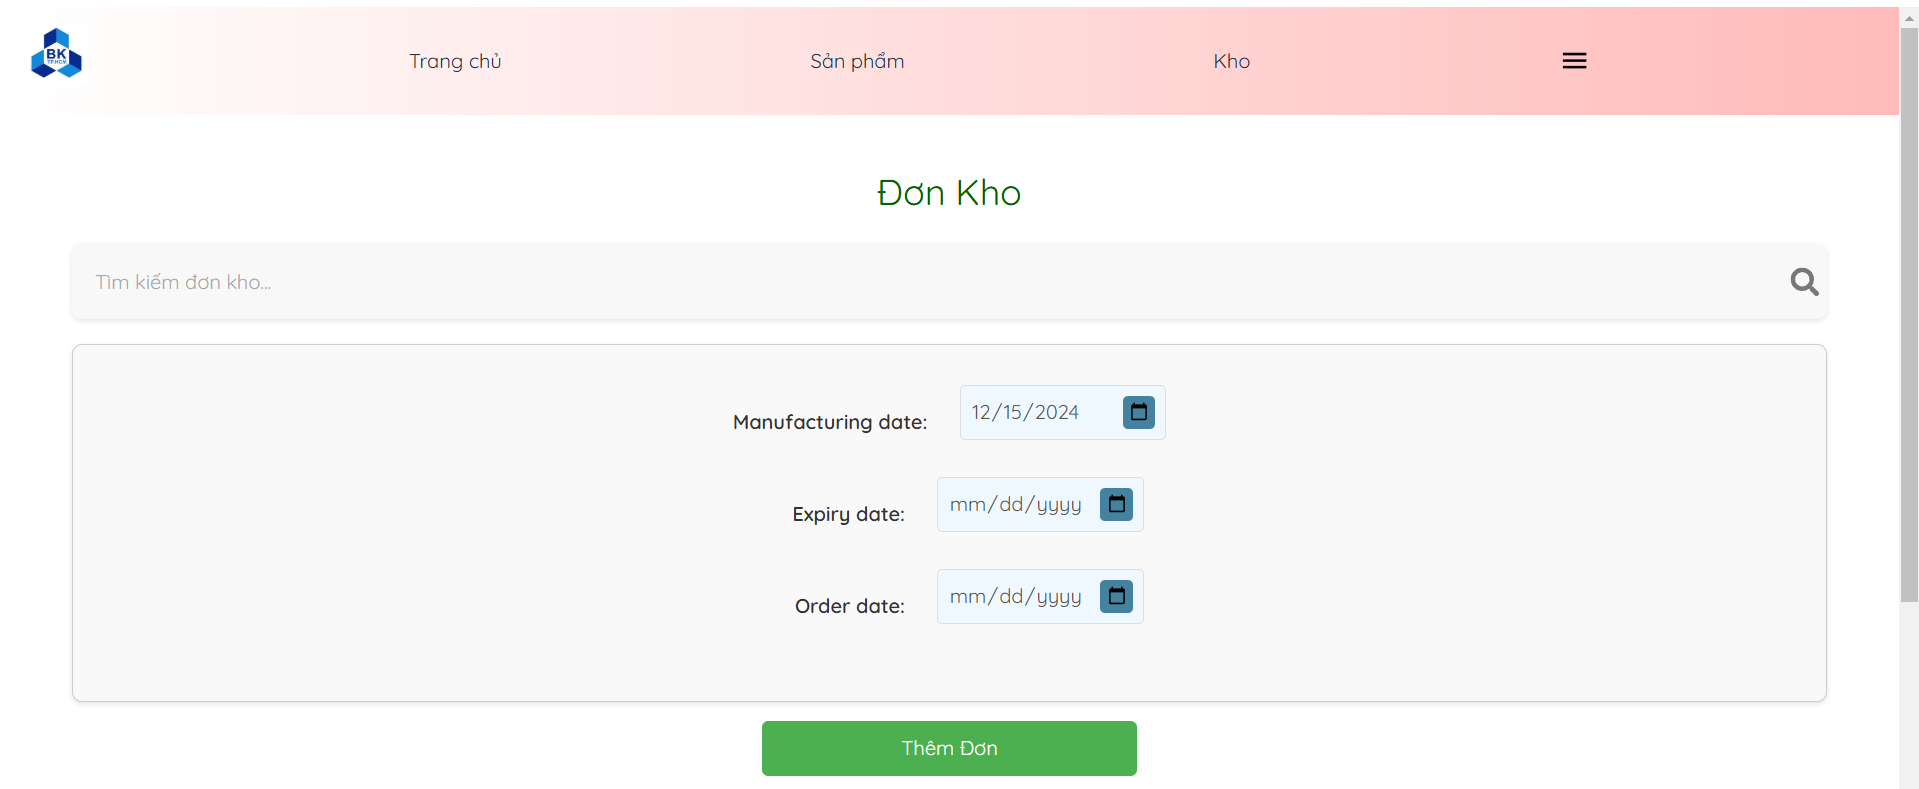
\includegraphics[scale=0.3]{Images/batch_warehouse/a2 (1).png}
    % \caption{Màn hình thêm sản phẩm}
    
\hspace*{-1cm}   
% \centering
    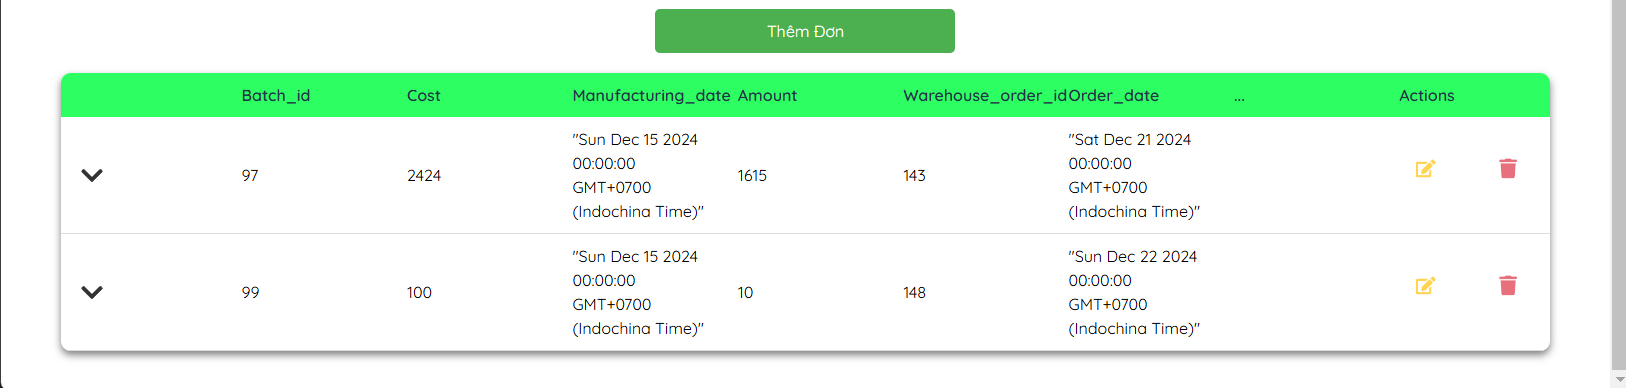
\includegraphics[scale=0.35]{Images/batch_warehouse/a2 (2).png}
    \caption{Màn hình xem thông tin lô hàng trong kho}
    
\end{figure}

\newpage

\begin{figure}[H]
\hspace*{-0.75cm}   
% \centering
    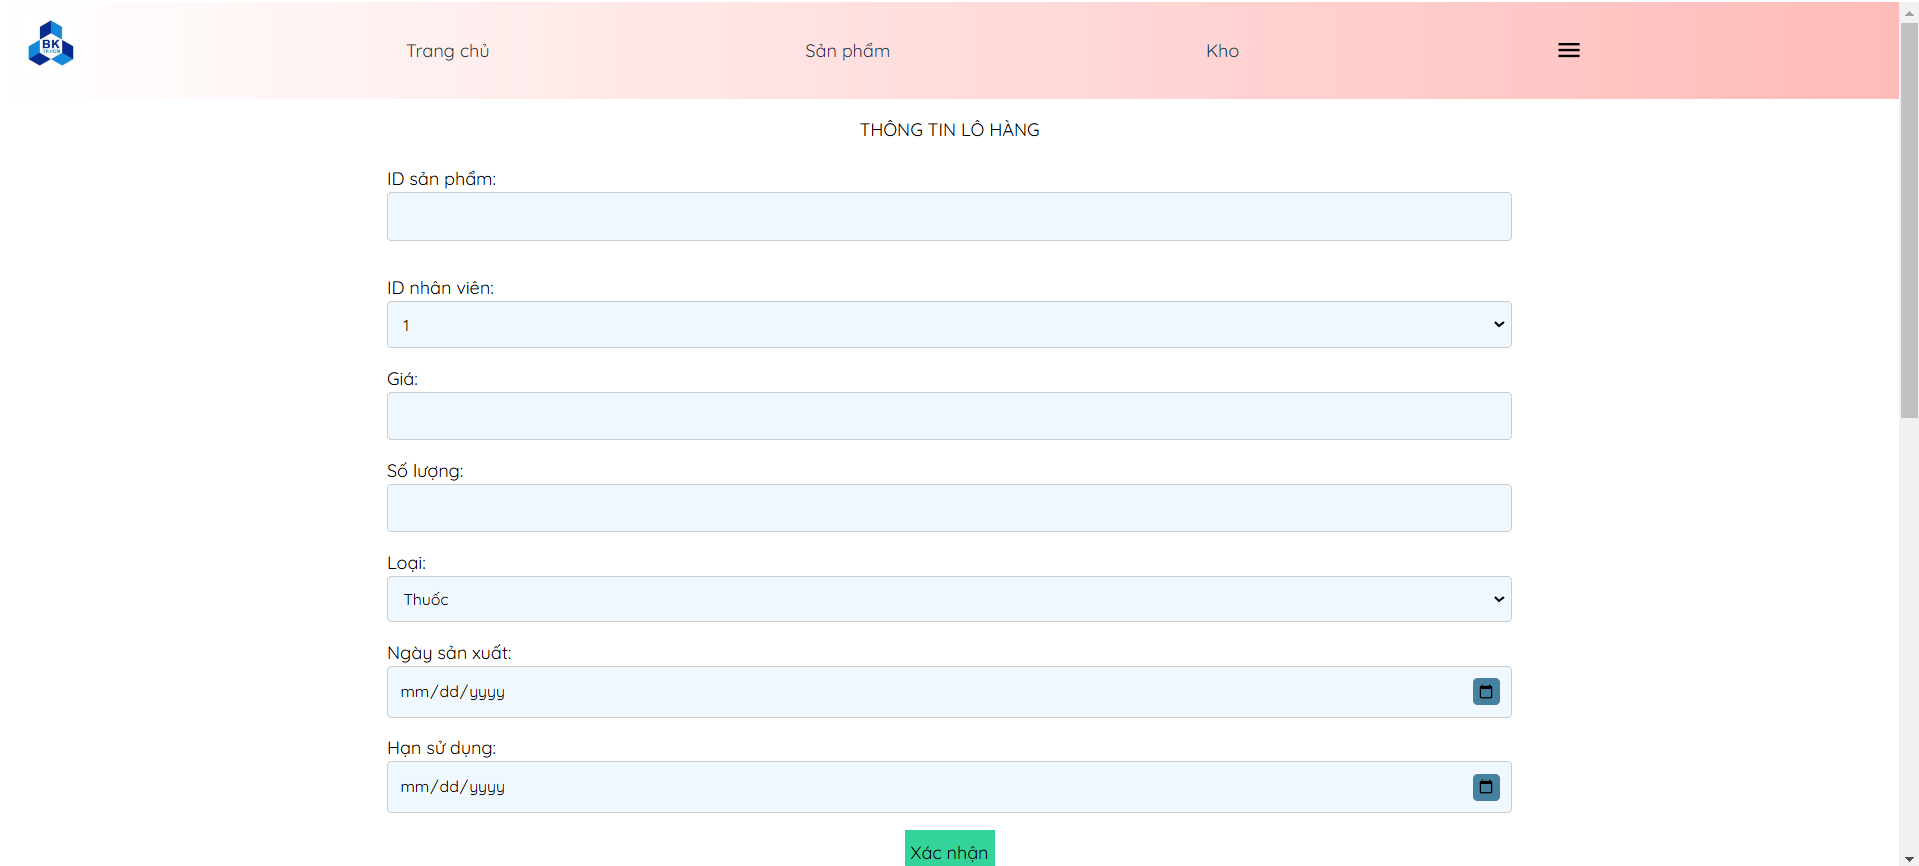
\includegraphics[scale=0.3]{Images/batch_warehouse/b3.png}
    \caption{Màn hình nhập thông tin lô}
    
\end{figure}

